% 서울대학교 전기컴퓨터공학부 석사 학위 논문에 맞추어 고침 
% 본 파일은 utf-8로 작성하여야 한다.
%
% by 김상훈
% 2008년 2월
% --------------------------------------------
% 서울대학교 수학과 학위 논문을 위한 논문 양식 뽄
% ver 0.9
% releasedate Oct 6th, 2005
% Copyleft. 어느 누구라도 마음대로 고치고 마음대로 배포할 수 있다.


% 배운 것을 정리하는 마음으로.....
% 2008년 2월
% 상훈

\documentclass[11pt, a4paper, oneside, openany, reqno]{book}

% book class 이외에 다른 클래스를 사용하여도 된다.
% 위의 옵션 중 [11pt, a4paper, oneside, openany] 은 반드시 필요하다.

%\usepackage{kotex}
\usepackage{document} %% 학위 논문 약식

% snumaththesis.sty 파일을 작성하고 있는 학위논문 TeX 파일과 같은 폴더에 복사해 놓으면 된다.
% amsmath, amssymb, amsthm, amsxtra, hfont 패키지들은 snumaththesis가 이미 불러온다.
% 따라서 이 패키지들을 별도로 불러올 필요는 없다.
%
% snumaththesis.sty 파일은 논문의 표지, 인준지 등을 만들어 주는 역할만 한다. 따라서
% 이 스타일 파일 이외에 어떠한 스타일 파일을 사용하더라도 서로 충돌하는 등의 문제는 없을 것이다.


% 문서에 그림을 삽입해야할 때
\usepackage{graphicx}
\usepackage{subfigure}	% 여러 그림을 넣는다

% 문서에 하이퍼 링크를 달고자 한다면 주석처리를 푼다.
\usepackage[colorlinks=true]{hyperref}

\hypersetup{%
pdftitle={blabla},%
pdfauthor={blabla},%
pdfkeywords={blabla},%
citecolor=black,%
filecolor=black,%
linkcolor=black,%
urlcolor=black,%
}

% [주의] pdfLaTeX을 이용하여 pdf 파일을 만들 때 하이퍼 링크와 책갈피가 모두 있는
%        문서를 만들고자 한다면, pdfLaTeX 컴파일을 적어도 두어 번 반복해야 한다.

% appendix의 소스 코드를 위해
\usepackage{fancyvrb}

% 아래는 theorem, corollary 등에 대한 기본적인 설정이다.
% 그대로 사용하거나 아래의 방법을 흉내어서 원하는대로 바꾸어 사용하면 된다.
% 참고 http://faq.ktug.or.kr/faq/AMSLaTeX?action=highlight&value=theorem

% theorem-like environment
% (사용 예) \newtheorem{환경이름}{화면에 나오는 이름}[번호 붙이는 방법]
% chapter 전체를 기준으로 번호가 붙는다. 즉 Theorem 1.1, Theorem 3.4와 같은 식으로 번호가 붙는다.
\newtheorem{theorem}{Theorem}[chapter] 
% Theorem과 번호를 공유한다. 즉, Corollary는 독자적인 번호를 갖지 않는다.
\newtheorem{corollary}[theorem]{Corollary} 
\newtheorem{lemma}[theorem]{Lemma}
\newtheorem{proposition}[theorem]{Proposition}
\newtheorem{question}{Question} % 독자적인 번호를 갖는다. Question 1, Question 2
\newtheorem{step}{Step}
\newtheorem{example}{Example}

% 번호를 붙이지 않는 `정리' 만들기
\newtheorem*{lemmawon}{Lemma}
\newtheorem*{claim}{Claim}

% 특별한 이름을 갖는, 번호가 붙지 않는 Theorem 만들기
\newtheorem*{questionA}{Question~A}
\newtheorem*{mainthmA}{Main Theorem~A}

% 본문의 글씨가 기울어지지 않는 환경
\theoremstyle{definition}
\newtheorem{definition}[theorem]{Definition}

% 화면에 나오는 이름이 이탤릭체인 환경
\theoremstyle{remark}
\newtheorem{remark}[theorem]{Remark}
\newtheorem{remarkof}{Remark}[theorem] % 어떤 Theorem의 아래에 Remark를 붙이고자 할 때.
\newtheorem*{remarkwon}{Remark}

% 수식 번호 붙이기
\numberwithin{equation}{chapter} % chapter 전체를 기준으로 번호가 붙는다. 즉 (1.1), (3.2)와 같이 붙는다.


% 내 명령어
\newcommand{\R}{\ensuremath{{\mathbb R}}}
\newcommand{\N}{\ensuremath{{\mathbb N}}}
\newcommand{\C}{\ensuremath{{\mathbb C}}}
\newcommand{\A}{\mathcal{A}}
\newcommand{\x}{\textbf{x}}
\newcommand{\y}{\textbf{y}}
\newcommand{\U}{\textbf{u}}
\newcommand{\NBR}{\mathcal{N}}
\newcommand{\ONE}{\textbf{1}}
\newcommand{\GRP}{\mathcal{G}}

\begin{document}
%% 본문 이전의 쪽들
\frontmatter


% 기초 정보 입력 
	% 영어 제목. 어쩔 수 없는 경우가 아니라면 수식 등을 사용하지 않는다.
	\EnglishTitle{Decentralized Formation Tracking Control of Multiple Homogeneous Agents}
	% 국어 제목. 어쩔 수 없는 경우가 아니라면 수식 등을 사용하지 않는다.
	\KoreanTitle{다 개체 동종 시스템의 분산 편대 추종 제어}
	% 지은이
	\AuthorKoreanName{김 상 훈}
	% 지은이 영어 이름
	\AuthorEnglishName{SANGHOON KIM}
	% 박사과정 학번
	\StudentNumber{2006-23150}
	% 국문학위명. 이학 박사 / 이학 석사
	\KoreanNameofDegree{공학석사}
	% 영문학위명. Doctor of Philosophy / Master of Science
	% Master of Engineering
	\EnglishNameofDegree{Master of Engineering}
	% 날짜 1학기 / 2학기
	% 학위 수여일. 2월 / 8월
	\GraduateDate{2008년 8월} %
	\GraduateDateEnglish{August 2008}
	% 심사용 논문 제출 기한. 4월 / 10월
	\SummittedDate{2008년 4월}
	% 종심 끝난 날짜. 6월 / 12월
	\RefereeDate{2008년 6월}
	% 논문 심사위원
	%
	% 석사논문 심사위원은 세 명이므로
	%    %\RefereeFourth{교수사}
	%    %\RefereeFifth{교수오}
	% 와 같이 주석처리한다.
	\RefereeChief{ }
	\RefereeSecond{ }
	\RefereeThird{ }
	%\RefereeFourth{교수사}
	%\RefereeFifth{교수오}
	% 지도교수 성명
	\AdvisorKoreanName{심 형 보}
	\AdvisorEnglishName{Hyungbo Shim}
	% Keywords. keyword는 논문을 검색할 때 색인어로 가능한 단어를 6개 이내로 선정
	\KeyWordsEnglish{output tracking, formation, decentralized control,
	feedback linearization, permutation, multiple homogeneous systems} 
	\KeyWordsKorean{추종 제어,편대 제어,분산 제어,궤한 선형화,다 개체 동종 시스템} 

	
% 각종 양식 만들기 
% 최종 제출 버젼이 아니라면 각종 양식은 필요없다.
% 이 경우에는 `각종 양식 만들기' 부분을 전부 주석처리하면 된다.
	% 앞표지 만들기
	\makefrontengcover	
	\newpage\thispagestyle{empty}\mbox{}\newpage
	\makefrontcover
	\newpage\thispagestyle{empty}\mbox{}\newpage
		
	% 국문 제출 승인서/인준지 만들기
	% \makeapproval
	\makeapprovalalt
	% 영문 제출 승인서
	%\makeenglishapproval
	% 학위논문 원문제공 서비스에 대한 동의서 만들기
	% 논문
	

	\newpage\thispagestyle{empty}\mbox{}\newpage
	\makewrittenconsent
	% the Copyright쪽 만들기
	\makecopyright{2008}


%% 영문초록.
%%
%% 1. 논문의 내용과 결론에 관하여 간략하고 구체적으로 기재
%%
%% 2. 스스로 정의한 수식, 명령어 등의 매크로를 사용하지 않는다.
%%    영문초록은  최소한의 설정 아래에서도
%%    아무런 문제없이 컴파일이 되어야 한다.
%%    그래야만 인터넷 등의 자동화 된 시스템에서 다른 이들도
%%    이 논문의 초록을 제대로 읽을 수 있기 때문이다.
%%
%% 3. 영문초록에서 논문의 각 chapter, section의 내용을 요약할 필요는 없다.
%%    왜냐하면 chapter, section의 내용 요약은 Introduction chapter에서 해야 하는 것이기 때문이다.
\begin{EnglishAbstract}
	Formation control of multiple agents has been studied by many researchers in recent years.
	Since lots of new applications have arisen, there is growing interest in this area for
	military systems, mobile sensor network, intelligent transportation systems and so on.
	Formation control has been exploited by a variety of methods 
	while many of formation approaches utilize the graph theory such as 
	Laplacian adjacency matrix to describe the interconnection of the agents.
	This representation also appears in consensus and synchronization problems
	with a similar analysis scheme.
	In this thesis, we focus on the formation tracking of multiple homogeneous nonlinear systems 
	by a decentralized manner. For time-varying smooth formation references, 
	the collection of the agents keeps the formation while the whole group can freely move anywhere
	regardless of the existence of leader of the group.
	One of the main goals is to achieve such a controller and to find the stability condition
	for formation tracking. And additionally, we discuss a permutation of the agents to get a benefit of
	the homogeneity of the collection.
\end{EnglishAbstract}



%% 쪽번호가 아래 중앙에 붙는다.
\pagestyle{fancy}%
\lhead{\leftmark}%
\rhead{}%
\chead{}%
\cfoot{\thepage}%
\renewcommand{\headrulewidth}{0pt}


%% 차례 만들기
%% 그림차례, 표 차례 등도 만들기 원한다면
%% 아래 \listoffigure, \listoftable의 주석표시를 지워라.
\addcontentsline{toc}{chapter}{Contents}
\tableofcontents
\addcontentsline{toc}{chapter}{List of Figures}
\listoffigures
\addcontentsline{toc}{chapter}{List of Tables}
%\listoftables


\chapter*{Notation and Symbols}
\addcontentsline{toc}{chapter}{Notation and Symbols}
\lhead{NOTATION AND SYMBOLS}
\begin{tabbing}
	$ \N $ \qquad\qquad\qquad\qquad  \= the set of all natural numbers\\
	$ \R $  \> the set of all real numbers\\
	$ \R^n $ \> the $ n $-dimensional Euclidean space\\
	$ \R^{n \times m} $  \> the space of $ m \times n $ matrices with real entries\\
	$ \C $  \> the set of all complex numbers\\
	$ \C^{n \times m} $  \> the space of $ m \times n $ matrices with complex entries\\
	$ \triangleq $  \> defined as \\
	$ L_f h(x)$ \> the Lie derivative of $h$ with respect to the vector field $f$,\\ 
	\> ($=\frac{\partial h}{\partial x} f(x)$) \\
	$ L_{f_1}L_{f_2}h $ \> $L_{f_1}(L_{f_2}h)$ \\
	$ L_f^i h $ \> $L_f L_f^{i-1} h $ \\ 
	$ L_f^1 h $ \> $L_f h $ \\
	$ L_f^0 h $ \> $h $ \\
	$ y^{(i)} $ \> the $ i $-th derivative of $ y $ with respect to time\\
	$ \therefore $ \> therefore \\
	$ \because  $ \> because \\
	$ \forall $ \> for all\\
	$ \exists $ \> there exists \\
	$ s.t. $ \> such that \\
	$ \in $ \> belong to\\
	$ \subset $ \> subset of\\
	$ \left[ 1 ,N \right] $ \> $\lbrace 1,2,3,\cdots, N \rbrace $\\
	$ \prod_{i \in A}f(i) $ \> product of the members $ f(i) $ \\
	$ \vert A \vert $ \> the cardinality of the set $ A $\\
	$ B \setminus A $ \> the set of all elements which are members of B, but not of A,\\ \> $(B-A)$\\
	$ \Vert x \Vert $ \> the norm of vector $ x $\\
	$ \Vert A \Vert $ \> the norm of matrix $ A $ \\
	$ \Vert A \Vert_F $ \> the Frobenius norm of matrix $ A $ \\
	$ A \circ B $	\> the elementwise product of the matrices\\ 
	$ f : S_1 \rightarrow S_2 $ \> a function $ f $ mapping a set $ S_1 $ into a set $ S_2 $\\
	$ f^{-1}(\cdot) $ \> the inverse of $ f $\\
	$ diag(A_1,\cdots,A_n) $ \> a block diagonal matrix with diagonal blocks $ A_1 $ to $ A_n $\\
	$ I_n $ \> the identity matrix of size $ n $ \\
	$ \ONE_n $ \> $ [1, \cdots, 1]^T $ \\
	$ P > 0 $ \> a positive definite matrix P \\
	$ P \geq 0 $ \> a positive semidefinite matrix P \\
	$ A^T $  \> the transpose of $ A $ \\
	$ A^H $  \> the Hermitian adjoint of $ A $, $ \bar{A}^T $ \\
	$ A \bigotimes B $ \> the Kronecker product with A by B\\
	$ tr(A) $ \> the trace of A\\
	$ A = \lbrace a_{ij} \rbrace $ \> the matrix A in which its $ (i,j) $ element is $ a_{ij} $ \\
	$ \square $ \> the end of proof\\
	$ \left[ \mathrm{xx} \right] $ \> see reference number xx in the bibliography \\
\end{tabbing}

\newpage\thispagestyle{empty}\mbox{}\newpage

%%% 본문 시작
\mainmatter
\lhead{\leftmark} % notation and symbol page를 위해 임시로 사용한 lhead를 대체
%%% 아래부터 직접 논문을 작성한다. \begin{document}는 이미 선언되어있으므로 내용만 적으면 된다.


%% 논문의 시작
%\part{part one title}


\chapter{Introduction}

Formation control of multiple agents has been studied by many researchers in recent years.
Since lots of new applications have arisen, there is growing interest in this area.
These applications include formation flight, 
cooperative classification, attack and rendezvous in military systems.
In mobile sensor network, 
environmental sampling and distributed observing 
are good examples as the application of the formation control.
Moreover, Intelligent transportation systems like automated highway system(AHS) 
and air traffic control have been investigated by many groups of the academy and the industry.
The recent survey \cite{surveycooperativecontrol} presents a readable overview of those applications.

Formation control has been exploited by a variety of methods.
In \cite{overlapping}, decentralized overlapping scheme was proposed 
for a formation of unmanned aerial vehicles which uses the mathematical framework of the inclusion principle
and the expansion of the dimensional space for interconnected systems.
In \cite{mesbahi}, Linear matrix inequalities (LMI) and graph theory were combined to deal with
formation flying control of multiple spacecraft.
Coordination of groups using nearest neighbors was studied in \cite{ali}
where each agent's heading is updated by a local rule based on the average of ones of its neighbors.
In \cite{SPL06}, cooperative control of steered agents was discussed in which the developed methodology
stabilizes isolated relative equilibria in identical systems moving in the plane.
And a tracking control for formation was researched in \cite{hsihan} 
through a sliding mode framework for a certain class of nonlinear systems.
Moreover, a distributed control scheme was suggested for formation of multiple robots without supervisor
in \cite{hiroaki}. And behavior-based formation control was explained in \cite{arkin}.
In addition, cooperation among a collection of vehicles using intervehicle communication
was analyzed in \cite{fax,glaff} which consider a formation problem as stabilization and 
provide a stability condition and a relation between the connectivity of agents and the stability.

Many of formation approaches utilize the graph theory such as 
Laplacian adjacency matrix to describe the interconnection of the agents.
This representation also appears in consensus and synchronization problems.
In \cite{weiren, weiren2, reza}, consensus under time varying interaction topologies was mentioned
where dynamical agents with fixed and switching network topology reach 
an agreement regarding a certain quantity of interest.
And synchronization of coupled systems was investigated in \cite{cww,cww2,amano,lucmoreau}.

In this thesis, we focus on a formation tracking of multiple homogeneous nonlinear systems 
by a decentralized manner. For time-varying smooth formation references, 
the collection of the agents keeps the formation while the whole group can freely move anywhere
regardless of the existence of leader of the group.
One of the main goals is to achieve such a controller and to find the stability condition
for formation tracking. And additionally, we discuss a permutation of the agents to get a benefit of
the homogeneity of the collection. The rest of this thesis is organized as follows.

In chapter $ 2 $, we discuss the output tracking control for nonlinear systems.
State feedback input-output linearization is employed to deal with the nonlinearity 
for both single-input single-output (SISO) and multi-input multi-output (MIMO) systems. 
And a simple static feedback controller is proposed for tracking a reference input.

In chapter $ 3 $, we extend the tracking controller to multiple homogeneous systems.
The first part of the chapter is briefly mentioned about tracking absolute references 
which is an easy case where the each agent of the group tracks individually its own reference.
The second part of the chapter is devoted to tracking relative references.
The output tracking problem of multiple homogeneous agents by relative references is
to design a controller which drives the differences of the outputs among the agents 
so as to track given references as shown below.
\begin{equation}
	\lim_{t \to \infty} \Vert \left( y_i(t) - y_j(t) \right) - y_{ijr}(t) \Vert = 0,
	\qquad 1\leq \forall i,j \leq N
\end{equation}
where $ N $ is the number of the agents,
$ y_i $, $ y_j $ are respectively the outputs of the agent $ i $, $ j $ 
and $ y_{ijr} $ is the reference for the difference of the outputs 
between the agent $ i $ and $ j $.
To simplify complexity to express equations for the collection of multiple homogeneous agents, 
we introduce Kronecker product and graph theory which includes Laplacian adjacency matrix.
The eigenvalues of Laplacian matrix play a key role for the stability of tracking references
which is analyzed by Perron Frobenius theorem and the property of the null space of Laplacian matrix.
In the last section of the chapter, 
the decentralized output tracking controller for relative references is developed
where each agent cannot sense all outputs of the agents but ones of only its neighborhoods.

Chapter $ 4 $ is composed of two parts about the formation tracking problem and
the permutation invariant formation tracking problem.
Before we discuss the formation tracking control, the common concept of formations is described. 
And the formation is mathematically defined as the matrix and the vector 
about relative outputs of the agents in the group with several examples.
The former formation tracking problem is to design a controller such that 
the relative output between the arbitrary two agents follows the formation reference,
which is resolved by applying the output tracking by relative references in the earlier chapter.
The latter permutation invariant formation tracking problem is to utilize the homogeneity of the agents.
Because the agents have the identical dynamics and we assume that all agents have the same ability 
to achieve a certain mission, each agent can be replaced by others.
For taking this advantage of homogeneity, a weighted graph matching problem is introduced 
with respect to the nearness in the sense of the included angle matching.
And we finally propose a formation tracking controller combined with the assignment dynamics
by which each agent goes through the nearest path to be in the formation.

In chapter $ 5 $, $ 6 $ agents of multiple homogeneous nonholonomic mobile robots are considered as an example.
And we verify the proposed controller well designed by simulating the collection of the mobile robots.

\chapter{Output Tracking of Nonlinear System}

In this chapter, we discuss the output tracking control for nonlinear systems.
State feedback input-output linearization is employed to deal with the nonlinearity 
for both single-input single-output and multi-input multi-output systems. 
And a simple static feedback controller is proposed for tracking a reference input.

\section{Single-Input Single-Output Case (SISO)}

\begin{definition}[Output Tracking Problem (SISO)]
	Consider the following single input single output systems with no uncertainties
	\begin{equation}\begin{split}\label{sisosys}
	\dot{x}&=f(x)+g(x)u,  \qquad x \in \R^n \\
	y&=h(x), \qquad\qquad\qquad y \in \R 
	\end{split}\end{equation} 
	with smooth $ f $ and $ g $ vector fields over $\R^n$ and $ h $: $\R^n \rightarrow \R$ 
	a smooth function s.t. $ h(0)=0 $.\\
	The \textbf{output tracking problem} is to design a controller with the property that,
	for given a smooth bounded reference signal $ y_r(t) $, the output of system satisfies 
	\[ \lim_{t \to \infty}(y(t)-y_r(t)) = 0 \]
	for any initial condition of the closed loop system.
\end{definition}

\subsection{Input-Output Feedback Linearization}

\begin{definition}[Input-Output Feedback Linearization]
	System \eqref{sisosys} is locally (globally) \textbf{state feedback input-output linearizable} 
	in a neighborhood of the origin $ U_0 $ (in $ \R^n $) if there exists a state feedback
	\begin{equation}
	u=k(x)+\beta(x)v
	\end{equation}
	with $k$ and $\beta$ smooth functions, 
	$\beta(x)\neq0, \forall x \in U_0 ( \forall x \in \R^n) $,
	such that the input-output dynamics of the closed loop system
	\begin{equation}\begin{split}\label{lsys}
	\dot{x}&= f(x) +g(x)(k(x)+\beta(x)v) \\
	y&= h(x)
	\end{split}\end{equation} 
	are given in $ U_0 ( \R^n )$ by \[ \frac{d^ry}{dt^r} = v \] with $ 1 \leq r \leq n $.
\end{definition}

\begin{remark}
	The output $ y $ of the system \eqref{lsys} is chained 
	to the input $ u $ with the $\rho$-th degree of integrators. 
	In the aspect of input $ v $ to output $ y  $, the system \eqref{lsys} is linear.
\end{remark}

\begin{definition}[Relative Degree $\rho$]
	The \textbf{(global) relative degree $\rho$ }of system \eqref{sisosys} is 
	defined as the integer s.t.
	\begin{equation}\begin{split}
	L_gL_f^ih(x)&=0 , \qquad\qquad \forall  0\leq i \leq  \rho -2 \\
	L_gL_f^{\rho{}-1}h(x)&\neq0, \qquad\qquad \forall x \in U_0 \quad( \forall x \in\R^n)
	\end{split}\end{equation} 
	where $ U_0 $ is a neighborhood of the origin.\footnote{Lie derivative of $h$ 
	with respect to $f = L_f h(x)=\frac{\partial h}{\partial x} f(x)$, 
	$ \quad L_{f_1}L_{f_2}h=L_{f_1}(L_{f_2}h)$, 
	$ \quad L_f^i h=L_f L_f^{i-1} h $, $ \quad L_f^1 h = L_f h $, $ \quad L_f^0 h = h $. }
	%If \begin{equation*}\begin{split}
	%L_gL_f^i h(x)&=0, \qquad\qquad  \forall i \geq 0 \\
	%\end{split}\end{equation*}
	%, then $ \rho=\infty $.
\end{definition}

\begin{remark}
	There might be a case where the relative degree cannot be defined.
\end{remark}

\begin{theorem}[State Feedback Linearized System]\label{lsysthm}
	Assume that the relative degree $ \rho $ is (globally) well defined.
	Then system \eqref{sisosys} is locally (globally) partially state feedback linearizable 
	with index $ \rho $ and is locally (globally) state feedback input-output linearizable, 
	i.e. locally (globally) feedback equivalent to:
	\begin{equation}\begin{split}\label{lform}
	\dot{\xi} &= \phi(\xi,z) , \qquad\qquad \xi \in \R^{n-\rho}\\
	\dot{z_i}&= z_{i+1} , \qquad\qquad 1 \leq i \leq \rho-1 \\
	\dot{z_\rho}&= v \\
	y &= z_1
	\end{split}\end{equation} 
	if and only if $ \rho \leq n $.
	Moreover, the feedback controller $ u $ is to be 
	\begin{equation}\label{nctrl}
	u = \frac{-L_f^\rho h(x)}{L_g L_f^{\rho-1} h(x)} + 
	\frac{1}{L_g L_f^{\rho-1} h(x)}v \triangleq k(x)+\beta(x)v
	\end{equation}
	%with $ \beta(0) \neq 0 $.
\end{theorem}

\begin{proof}
	See the proof in \cite{marino}.
\end{proof}

%\begin{remark}
%Equation \eqref{lform} is called \textbf{normal form}.
%\end{remark}

\begin{remark} 
	System \eqref{sisosys} is globally state feedback input-output linearizable 
	if, and only if the vector fields
	\begin{equation} \label{vfield}
	\tilde{f} \triangleq f+\frac{-L_f^\rho h(x)}{L_g L_f^{\rho-1} h(x)}g,
	\qquad\qquad \tilde{g} \triangleq \frac{1}{L_g L_f^{\rho-1} h(x)}g
	\end{equation}
	are complete\footnote{A vector field $ f(x) $ is said to be \textbf{compelete} 
	if the solutions to the differential equation $ \dot{x}=f(x) $ 
	may be defined for all $ t \in \R $ }.
\end{remark}

\begin{definition}[Zero Dynamics]
	Assume that $\rho \leq n$ in $ U_0  $ for system \eqref{sisosys}.\\
	Let $ z_i = L_f^{i-1} h(x), 1 \leq i \leq \rho $. Define the $ (n-\rho) $-dimensional manifold 
	$ M=\lbrace x \in U_0 : h(x) =0,\cdots,L_f^{\rho-1}h(x)=0\rbrace $.
	The dynamics of system \eqref{sisosys} constrained in M are called the \textbf{zero dynamics}.
\end{definition}

\begin{remark}
	The zero dynamics of system \eqref{sisosys} are given with equation \eqref{lform} by 
	\begin{equation}
	\dot{\xi} = \phi(\xi,0) , \qquad\qquad \xi \in \R^{n-\rho}
	\end{equation}
\end{remark}

\begin{definition}[Minimum Phase]
	System \eqref{sisosys} with $ \rho \leq n $ is called \textbf{minimum phase} 
	if the origin $ \xi=0 $	is an asymptotically stable equilibrium point for the zero dynamics. 
	A system which is not minimum phase
	is said to be \textbf{non-minimum phase}.
\end{definition}

\begin{remark}
	If the relative degree $ \rho $ is equal to the dimension $ n $ of $ x $, 
	then there are no $ \xi $ terms in \eqref{lform}. (i.e.  no zero dynamics), 
	in which the set of functions $ z_i = L_f^{i-1} h(x) \quad (1 \leq i \leq n$)  
	completely define a coordinates transformation.
\end{remark}

\subsection{Output Tracking}

\begin{definition}[Tracking Dynamics]
	Assume that it is $ \rho \leq n $ in $ U_0 $ for system \eqref{sisosys} 
	and there exists an initial condition $ x_0 \in U_0$ 
	which is compatible\footnote{The initial condition $ x(0)=x_0 \in U_0 $ 
	is said to be \textbf{compatible} 
	with the reference signal $ y_r (t) $ for system \eqref{sisosys} 
	if $ y_r^{(i)} (0) = L_f^i h(x_0), 0 \leq i \leq \rho -1 $} 
	with the reference signal $ y_r(t) $. Let \\
	\begin{equation}
	M_t = \lbrace x \in U_0 : h(x) = y_r(t),\cdots , L_f^{\rho-1} h(x) = y_r^{(\rho-1)}(t) \rbrace
	\end{equation}
	be the time-varying $ (n-\rho) $ -dimensional integral manifold called the tracking manifold. 
	The dynamics of system \eqref{sisosys} which are subjected to constraints $ M_t $ are said to be
	the \textbf{tracking dynamics}.
\end{definition}

\begin{theorem}[Tracking Control \cite{marino}]
	For system \eqref{sisosys}, 
	assume that the global relative degree is well defined with $ \rho \leq n $,
	the vector fields \eqref{vfield} are complete, 
	and the tracking dynamics are bounded input bounded state stable. If 
	\begin{equation}\label{sisohurwiz}
	s^\rho + k_\rho s^{\rho-1} + \cdots + k_1
	\end{equation}
	is a Hurwitz polynomial\footnote{A polynomial is called a \textbf{Hurwitz polynomial} 
	if all its roots have negative real parts.}, 
	then the tracking problem is globally solvable 
	by static state feedback controller $ u $ in \eqref{nctrl} with 
	\begin{equation}\label{sisov}
	v= -k_1(z_1 - y_r (t)) - \cdots - k_\rho (z_\rho - y_r^{(\rho -1)}(t)) + y_r^{(\rho)} (t)
	\end{equation}
\end{theorem}

\begin{proof}
	If system \eqref{sisosys} has a well defined relative degree $ \rho $, 
	then it satisfies the conditions of 
	Theorem \ref{lsysthm}. thus, the control \eqref{nctrl} is globally well defined.
	In that case, one takes $ v $ as the equation \eqref{sisov}, we obtain
	\begin{equation}
	\left[\begin{array}{c}
	\dot{e_{1}}\\
	\vdots\\
	\dot{e_{\rho-1}}\\
	\dot{e_{\rho}}\end{array}\right]=\left[\begin{array}{cccc}
	0 & 1 & \cdots & 0\\
	\vdots & \vdots & \ddots & \vdots\\
	0 & 0 & \cdots & 1\\
	-k_{1} & -k_{2} & \cdots & -k_{\rho}\end{array}\right]\left[\begin{array}{c}
	e_{1}\\
	\vdots\\
	e_{\rho-1}\\
	e_{\rho}\end{array}\right]
	\end{equation}
	with $ e_i \triangleq z_i -y_r^{(i-1)} = y^{(i-1)}-y_r^{(i-1)} $. 
	In the assumption, we have the Hurwitz polynomial \eqref{sisohurwiz}, 
	finally asymptotic tracking is achieved 
	for any initial error $ e(0) $. Since $ y_r, \cdots,y_r^{\rho} $ are bounded, 
	it follows that $ z_1, \cdots, z_\rho $ are bounded. 
	Because of the property of the bounded input bounded state stability of the tracking dynamics, 
	$ \xi  $ from \eqref{lform} is bounded as well, $ z_1 (t), \cdots, z_\rho (t) $
	as bounded  references.
\end{proof}

\section{Multi-Input Multi-Output Case (MIMO)}

\begin{definition}[Output Tracking Problem (MIMO)]
	Consider the following multi-input multi-output systems with no uncertainties
	\begin{equation} \begin{split}\label{mimosys}
	\dot{x}&= f(x)+g(x)u,  \qquad \qquad x \in \R^n \\
	y&=h(x), \qquad\qquad\qquad\qquad y \in \R^m 
	\end{split}\end{equation} where
	\begin{alignat*}{3}
	u&=\left[u_1 ,\cdots ,u_m\right]^T ,  \qquad & u & \in \R^m \\
	%g(x)&=\left[g_1 (x) ,\cdots ,g_m (x) \right]   \qquad & g(x) & \in \R^{n \times m} \\
	g(x)&=\left[ \begin{array}{ccc}
	\vert & & \vert \\
	g_1 (x), & \cdots , & g_m (x) \\
	\vert & & \vert \\
	\end{array} \right],   \qquad & g(\cdot) & \in \R^{n \times m} \\
	h(x)&=\left[h_1 (x) ,\cdots ,h_m (x) \right]^T , \qquad & h(\cdot) & \in \R^m 
	\end{alignat*} 
	with smooth $ f $ and $ g_1 ,\cdots g_m $ vector fields over $\R^n$ 
	and $ h_i $: $\R^n \rightarrow \R$ 
	a smooth function s.t. $ h_i(0)=0 \quad (0 \leq i \leq m) $. 

	The \textbf{output tracking problem} is to design a controller with the property that,
	for a given smooth bounded reference signal $ y_r(t) \in \R^m$, the output of system satisfies 
	\[ \lim_{t \to \infty}\Vert y(t)-y_r(t) \Vert = 0 \]
	for any initial condition of the closed loop system.
\end{definition}

\subsection{Input-Output Feedback Linearization}

\begin{definition}[Input-Output Feedback Linearization]
	System \eqref{mimosys} is locally (globally) \textbf{state feedback input-output linearizable} 
	in a neighborhood of the origin $ U_0 $ (in $ \R^n $) if there exists a state feedback
	\begin{equation}
	u=k(x)+\beta(x)v
	\end{equation}
	where $v=\left[v_1 ,\cdots ,v_m\right]^T  \in \R^m $ with a smooth vector field $k(x)$ 
	and smooth nonsingular $\beta(x) \in \R^{m \times m}$  matrix 
	for $ \forall x \in U_0 ( \forall x \in \R^n) $,
	such that the input-output dynamics of the closed loop system
	\begin{equation}\begin{split}\label{mimolsys}
	\dot{x}&= f(x) +g(x)(k(x)+\beta(x)v) \\
	y&= h(x)
	\end{split}\end{equation} 
	are given in $ U_0 ( \R^n )$ by 
	\[ \frac{d^{r_{i}}y_i}{dt^{r_i}} = v_i \] with $ 1 \leq r_1 + \cdots + r_m \leq n $ 
	for  $ 1 \leq \forall i \leq m $.
\end{definition}


\begin{definition}[Vector Relative Degree $\rho$]
	The \textbf{(global) vector relative degree $\rho$ }of system \eqref{mimosys} is defined as 
	the vector $ \rho=\left[ \rho_1,\cdots,\rho_m \right]^T \in \N^{m} $ s.t. 
	\begin{equation}\begin{split}
	& L_{g_{j}} L_f^k h_i (x) =0, \\
	& \A (x)=\left[\begin{array}{ccc}
	L_{g_1} L_f^{\rho_1 -1} h_1 (x) & \cdots & L_{g_m} L_f^{\rho_1 -1} h_1 (x)\\
	L_{g_1} L_f^{\rho_2 -1} h_2 (x) & \cdots & L_{g_m} L_f^{\rho_2 -1} h_2 (x)\\
	\vdots & \ddots & \vdots\\
	L_{g_1} L_f^{\rho_m -1} h_m (x) & \cdots & L_{g_m} L_f^{\rho_m -1} h_m (x)\\\end{array}\right], \\
	\end{split}\end{equation} 
	for  $ 1 \leq \forall j \leq m ,\quad 0\leq \forall  k \leq \rho_i -2 , 
	\quad 1 \leq \forall i \leq m, \quad \forall x  \in U_0 \,(\forall x \in \R^n ) $ \\
	where $ U_0 $ is a neighborhood of the origin and\\
	$ \A (\cdot) \in \R^{m \times m}$ is nonsingular at $ x \in U_0 $ (nonsingular at $ x \in \R^n $). 
\end{definition}

\begin{theorem}[State Feedback Linearized System]\label{mimolsysthm}
	Assume that the vector relative degree $ \rho $ is (globally) well defined.
	Then system \eqref{mimosys} is locally (globally) partially state feedback linearizable 
	with indices $\lbrace \rho_1, \cdots, \rho_m \rbrace$ 
	and is locally (globally) state feedback input-output linearizable, 
	i.e. locally (globally) feedback equivalent to:
	\begin{equation}\begin{split}\label{mimolform}
	\dot{\xi} &= \phi(\xi,z,v) , \qquad\qquad\qquad\qquad \xi \in \R^{n-\rho^*}\\
	\dot{z_{1i_1}}&= z_{1i_1+1} , \quad \dot{z_{1\rho_1}}= v_1,  \qquad\qquad 1 \leq i_1 \leq \rho_1 -1 \\
	\dot{z_{2i_2}}&= z_{2i_2+1} , \quad \dot{z_{2\rho_2}}= v_2,  \qquad\qquad 1 \leq i_2 \leq \rho_2 -1 \\
	\vdots \\
	\dot{z_{mi_m}}&= z_{mi_m+1} , \quad \dot{z_{m\rho_m}}= v_m,  \qquad\quad 1 \leq i_m \leq \rho_m -1 \\
	y &= \left[ z_{11}, z_{21}, \cdots , z_{m1}  \right]^T
	\end{split}\end{equation} 
	if and only if $ \rho^* \triangleq \rho_1 + \rho_2 + \cdots + \rho_m \leq n $.
	Moreover, the feedback controller $ u $ is to be 
	\begin{equation}\begin{split}\label{mimonctrl}
	u &= -\A^{-1}(x)
	\left[ \begin{array}{c}L_f^{\rho_1} h_1\\ L_f^{\rho_2} h_2\\ \vdots\\ 
	L_f^{\rho_m} h_m\end{array} \right] + \A^{-1}(x)v \\
	& \triangleq k(x)+\beta(x)v, \qquad\qquad\qquad k(\cdot) \in \R^{m}, \quad
	\beta(\cdot) \in \R^{m \times m} \\
	\end{split}\end{equation} 
	where $ v= \left[ v_1, \cdots, v_m \right]^T $.
\end{theorem}

\begin{proof}
	See the proof in \cite{khalil, isidori, marino}.
\end{proof}

\begin{remark} 
	Equation \eqref{mimolform} has the Brunovsky canonical form. i.e.
	\begin{equation}\begin{split}
	\dot{z}&=Az+Bv \\
	y&= Cz\\
	\end{split}\end{equation} 
	where 
	\begin{equation}\begin{split}\label{brunovsky}
	z&=\left[z_{11},z_{12},\cdots,z_{1\rho_1},\cdots\cdots, z_{m1}, z_{m2}, \cdots, z_{m\rho_m} \right] ^T \\ 
	A&=diag(A_1, \cdots , A_m) \in \R^{\rho^* \times \rho^*},
	\qquad B=diag(B_1,\cdots,B_m) \in \R^{\rho^* \times m}, \\
	C&=diag(C_1, \cdots , C_m) \in \R^{m \times \rho^*},\\
	\end{split}\end{equation} 
	\begin{equation*}\begin{split}
	& A_i= \left[ \begin{array}{ccccc}
	0 & 1 & 0 & \cdots & 0\\
	0 & 0 & 1 & \cdots & 0\\
	\vdots & & & \ddots & \vdots \\
	0 & 0 & 0 & \cdots & 1 \\
	0 & 0 & 0 & \cdots & 0 \\
	\end{array} \right]  \in \R^{\rho_i \times \rho_i}, \quad
	B_i = \left[\begin{array}{c}0 \\ 0 \\ \vdots \\ 0  \\ 1  \\ \end{array} \right]  \in \R^{\rho_i} ,\\
	& C_i=\left[ 1, 0, \cdots, 0 \right] \in \R^{1 \times \rho_i} \\
	& \mathrm{for} \quad 1 \leq i \leq m \\
	\end{split}\end{equation*} 
\end{remark}

%\begin{remark} Distribution, involutive \end{remark}
%\begin{remark} Full state input-output linearization \end{remark}


\begin{remark} 
	System \eqref{mimosys} is globally state feedback input-output linearizable 
	if, and only if the vector fields
	\begin{equation} \label{mimovfield}
	\tilde{f} \triangleq f+gk(x),
	\qquad\qquad \tilde{g_i} \triangleq g\beta_i (x),
	\qquad 1 \leq i \leq m
	\end{equation}
	are complete where $ \beta_i(x) $ is the $ i $-th column vector of  $\beta (x)$.
\end{remark}

\begin{definition}[Zero Dynamics]
	Assume that $\rho^* \leq n$ in $ U_0  $ for system \eqref{mimosys}.\\
	Let $ z_{1i_1}=L_f^{i_1-1}h_1(x), \cdots\cdots, z_{mi_m}=L_f^{i_m-1}h_m(x) $ ,
	$ 1 \leq i_j \leq \rho_j $. 
	Define the $ (n-\rho^*) $-dimensional manifold 
	$ M=\lbrace x \in U_0 : h_1(x) =0,\cdots,L_f^{\rho_1-1} h_1(x)=0,\cdots,
	h_m(x) =0,\cdots,L_f^{\rho_m-1} h_m(x)=0 \rbrace $.
	The dynamics of system \eqref{mimosys} constrained in M are called the \textbf{zero dynamics}.
\end{definition}

\begin{remark}
	The zero dynamics of system \eqref{mimosys} are given with equation \eqref{mimolform} by 
	\begin{equation}
	\dot{\xi} = \phi(\xi,0,0), \qquad\qquad \xi \in \R^{n-\rho^*}
	\end{equation}
\end{remark}

\begin{definition}[Minimum Phase]
	System \eqref{mimosys} with $ \rho^* \leq n $ is called \textbf{minimum phase} 
	if the origin $ \xi=0 $	is an asymptotically stable equilibrium point for the zero dynamics. 
	A system which is not minimum phase is said to be \textbf{non-minimum phase}.
\end{definition}

\subsection{Output Tracking}


\begin{definition}[Tracking Dynamics]
	Assume that $ \rho^* \leq n $ in $ U_0 $ for system \eqref{mimosys} 
	and that there exists an initial condition $ x_0 \in U_0$ 
	which is compatible\footnote{The initial condition $ x(0)=x_0 \in U_0 $ 
	is said to be \textbf{compatible} with the reference signals 
	$ y_{1r} (t),\cdots,y_{mr} (t) $ for system \eqref{mimosys} 
	if $ y_{1r}^{(i_1)} (0) = L_f^{i_1} h_1(x_0), \cdots, 
	y_{mr}^{(i_m)} (0) = L_f^{i_m} h_m(x_0) \quad 0 \leq i_j \leq \rho_j -1 $} 
	with the reference signals $ y_{1r}(t),\cdots, y_{mr}(t) $. Let \\
	\begin{equation}\begin{split}
	M_t = \lbrace x \in U_0 : &  h_1(x) = y_{1r}(t),\cdots , 
	L_f^{\rho_1-1} h_1 (x) = y_{1r}^{(\rho_1-1)}(t),\cdots\cdots,\\
	& h_m(x) = y_{mr}(t),\cdots , L_f^{\rho_m-1} h_m (x) = y_{mr}^{(\rho_m-1)}(t) \rbrace \\
	\end{split}\end{equation} 
	be the time-varying $ (n-\rho^*) $ -dimensional integral manifold called the tracking manifold. 
	The dynamics of system \eqref{mimosys} which are subjected to constraints $ M_t $ are said to be
	the \textbf{tracking dynamics}.
\end{definition}

\begin{theorem}[Tracking Control]\label{trackingthm}
	For the system \eqref{mimosys}, 
	assume that the global vector relative degree $ \rho $ is well defined with $ \rho^* \leq n $,
	the vector fields \eqref{mimovfield} are complete, 
	and the tracking dynamics are bounded input bounded state stable. If 
	\begin{equation}\begin{split}\label{mimohurwitz}
	&s^{\rho_1} + k_{1\rho_1} s^{\rho_1-1} + \cdots + k_{11}, \\
	&\qquad\qquad\qquad\vdots \\
	&s^{\rho_m} + k_{m\rho_m} s^{\rho_m-1} + \cdots + k_{m1} \\
	\end{split}\end{equation} 
	are Hurwitz polynomials, 
	then the tracking problem is globally solvable 
	by static state feedback controller $ u $ in \eqref{mimonctrl} with 
	\begin{equation}\begin{split}\label{mimov}
	v_1& = -k_{11}(z_{11} - y_{1r} (t)) - \cdots 
	- k_{1\rho_1} (z_{1\rho_1} - y_{1r}^{(\rho_1 -1)}(t)) + y_{1r}^{(\rho_1)} (t) \\
	&\qquad\qquad\qquad\qquad\qquad\qquad\qquad \vdots \\
	v_m& = -k_{m1}(z_{m1} - y_{mr} (t)) - \cdots 
	- k_{m\rho_m} (z_{m\rho_m} - y_{mr}^{(\rho_m -1)}(t)) + y_{mr}^{(\rho_m)} (t) \\
	\end{split}\end{equation} 
\end{theorem}

\begin{proof}
	If system \eqref{mimosys} has a well defined vector relative degree 
	$ \rho=\left[ \rho_1, \cdots, \rho_m \right]^T $, 
	then it satisfies the conditions of Theorem \ref{mimolsysthm}. 
	Thus, the control \eqref{mimonctrl} is globally well defined.
	In that case, one takes $ v $ as the equation \eqref{mimov}, then we obtain
	\begin{equation}
	\left[\begin{array}{c}
	\dot{e_{i1}}\\
	\vdots\\
	\dot{e_{i\rho_{i-1}}}\\
	\dot{e_{i\rho_i}}\end{array}\right]=\left[\begin{array}{cccc}
	0 & 1 & \cdots & 0\\
	\vdots & \vdots & \ddots & \vdots\\
	0 & 0 & \cdots & 1\\
	-k_{i1} & -k_{i2} & \cdots & -k_{i\rho_i}\end{array}\right]\left[\begin{array}{c}
	e_{i1}\\
	\vdots\\
	e_{i\rho_{i-1}}\\
	e_{i\rho_i}\end{array}\right],
	\quad 1 \leq \forall i \leq m
	\end{equation}
	with $ e_{ij} \triangleq z_{ij} -y_{ir}^{(j-1)} = y_i^{(j-1)}-y_{ir}^{(j-1)} $. 
	In the assumptions, we have Hurwitz polynomials \eqref{mimohurwitz}, 
	asymptotic tracking is finally achieved for any initial error 
	$ e(0) $. Since $ y_{ir}, \cdots,y_{ir}^{\rho_i} $ are bounded, it follows that 
	$ z_{i1}, \cdots, z_{i\rho_i} $ are bounded. 
	Because of the property of the bounded input bounded state stability of the tracking dynamics, 
	$ \xi  $ from \eqref{mimolform} is bounded as well, $ z_{i1} (t), \cdots, z_{i\rho_i} (t) $
	as bounded references.
\end{proof}


\chapter{Output Tracking of Multiple Homogeneous Agents}
%In this section, we propose the method to deal with multiple homogeneous agents for tracking problem. 
%At the first, the method is presented that is using absolute outputs of agents, 
%and the second one follows that is using only relative outputs of agents.%, which is a decentralized scheme.
In this chapter, 
we extend the tracking controller discussed in the earlier chapter to multiple homogeneous systems.
The first part of the chapter is briefly mentioned about the output tracking by absolute references 
where the each agent of the group tracks individually its own reference.
And the second part of the chapter is devoted to the output tracking by relative references
which is utilized for the formation tracking control in the next chapter.

Consider the following N systems of multiple homogeneous\footnote
{They have an identical dynamics.} agents.
% i.e. $ x_1 = f(x_1)+g(x_1)u_1,\cdots,x_N = f(x_N)+g(x_N)u_N $} 
\begin{equation}\begin{split}\label{multisys}
	\dot{x_1} &=f(x_1)+g(x_1)u_1, \qquad\qquad  y_1 = h(x_1), \\
	\dot{x_2} &=f(x_2)+g(x_2)u_2, \qquad\qquad  y_2 = h(x_2),\\
	& \qquad \qquad \vdots \\
	\dot{x_N} &=f(x_N)+g(x_N)u_N, \qquad\quad  y_N = h(x_N),\\
\end{split}\end{equation} 
where
\begin{alignat*}{3}
	u_i&=\left[u_{i1} ,\cdots ,u_{im}\right]^T ,  \qquad & u_i & \in \R^m \\
	%g(x)&=\left[g_1 (x) ,\cdots ,g_m (x) \right]   \qquad & g(x) & \in \R^{n \times m} \\
	g(x_i)&=\left[ \begin{array}{ccc}
	\vert & & \vert \\
	g_1 (x_i), & \cdots, & g_m (x_i) \\
	\vert & & \vert \\
	\end{array} \right],   \qquad & g(\cdot) & \in \R^{n \times m} \\
	h(x_i)&=\left[h_1 (x_i) ,\cdots ,h_m (x_i) \right]^T , \qquad & h(\cdot) & \in \R^m  
\end{alignat*} 
with $ x_i \in \R^n $,  
smooth $ f $ and $ g_1 ,\cdots, g_m $ vector fields over $\R^n$ 
and $ h_j $: $\R^n \rightarrow \R$ 
a smooth function s.t. $ h_j(0)=0 $ for
$ 1 \leq \forall i \leq N $ and $ 0 \leq \forall j \leq m $. 


\section{Output Tracking by Absolute References}

At first, we consider the case that every references are given by absolute values.
In such cases, straightforwardly, one can get the controller 
which lets the outputs of the corresponding agent track its own reference signals 
by the method in which an individual agent independently tracks its reference.

\begin{definition}
	The \textbf{output tracking problem of multiple homogeneous agents by absolute references} 
	is to design a controller with the property that, 
	for given a smooth bounded reference signal $ y_{ir}(t) \in \R^m$, 
	the outputs of systems \eqref{multisys} satisfies 
	\begin{equation}
	\lim_{t \to \infty}\Vert y_i(t)-y_{ir}(t) \Vert = 0, \qquad 1\ \leq \forall i \leq N 
	\end{equation}	
	for any initial condition of the closed loop system.
\end{definition}

\begin{theorem}
	For each agent system of multiple homogeneous agent systems \eqref{multisys}, 
	assume that the global vector relative degree $ \rho $ is well defined with $ \rho^* \leq n $, 
	% the vector fields \eqref{mimovfield} are complete, 
	and the tracking dynamics are bounded input bounded state stable. 
	If the references for systems \eqref{multisys} are given by absolute values,
	then the tracking problem is globally solvable.
\end{theorem}

\begin{proof}
	For each agent system in systems \eqref{multisys}, choose $ k_{ij} $ such as \eqref{mimohurwitz}. 
	By Theorem \ref{trackingthm}, we can independently solve the tracking problem for each agent.
	Thus, the case of multiple agents is also solved.
\end{proof}

\begin{remark}
	For a tracking dynamics, bounded input bounded state stabilty can be replaced with
	the term of the input-to-state stability (ISS).
\end{remark}

\section{Output Tracking by Relative References}

Now, we consider the references that are given by relative values.

\begin{definition}
	The \textbf{output tracking problem of multiple homogeneous agents by relative references} is 
	to design a controller with the property that, 
	for given a smooth bounded relative reference signal $ y_{(ij)r}(t) \in \R^m$, 
	the outputs of systems \eqref{multisys} satisfies 
	\begin{equation}\label{defreltrack}
	\lim_{t \to \infty}\Vert (y_i(t) - y_j(t)) - y_{(ij)r}(t) \Vert = 0, 
	\qquad 1\ \leq \forall i,j \leq N 
	\end{equation}
	for any initial condition of the closed loop system.
\end{definition}

For multiple systems \eqref{multisys}, if the references are given by relative values,
bearing in mind of relativeness, one can redefine each output of the agent system in \eqref{multisys}
as follows, 
\begin{equation}\label{newout}
y_i^* =\sum_{j \in \NBR_i}w_{ij}(y_i-y_j), \qquad  1 \leq \forall i \leq N\\
\end{equation} 
where $ \NBR_i \subset [1,N] \setminus \lbrace i \rbrace $ is the index set that represents
the set of agents which the agent $ i $ can sense, and $ w_{ij} $ is a scalar for weighting.

For each system of multiple systems \eqref{multisys}, 
if its own output of the agent can be absolutely measurable by itself\footnote
{Someone in a moving elevator could not get one's absolute position by oneself
without an additional information from the elevator.} 
and the vector relative degree is well defined, 
(i.e. for $ i $-th agent, the well defined vector relative degree with respect to $ u_i $ and $ y_i $ ),
each agent system can be state feedback input output linearizable.

Using the new outputs of each agents and the input-output linearizability, 
the whole system dynamics are represented as follows

\begin{theorem}\label{brusysthm}
	For the collection of multiple homogeneous agents systems \eqref{multisys}, 
	assume that the global vector relative degree $ \rho $ is well defined with $ \rho^* \leq n $, 
	the vector fields \eqref{mimovfield} are complete, 
	and the references for systems \eqref{multisys} 
	are given by relative values.
	If the output of each agent system can be absolutely measurable by itself,
	then systems \eqref{multisys} can be represented with new outputs such that \eqref{newout} as follows.
	\begin{equation}\begin{split}\label{brusys}
	\dot{\xi_i} &= \phi(\xi_i,z_i,v_i), \\
	\dot{z_i}&=Az_i+Bv_i, \\
	y_i^* & =\sum_{j \in \NBR_i}w_{ij}(Cz_i-Cz_j), \qquad  1 \leq \forall i \leq N\\
	\end{split}\end{equation} 
	where $ A,B,C $ are defined as \eqref{brunovsky}.
\end{theorem}

\begin{proof}
	By the assumption, one can apply Theorem \ref{mimolsysthm} 
	to each agent of systems \eqref{multisys}, 
	and replace each output with new output \eqref{newout}.
\end{proof}

%\begin{theorem}
%미리 선형화 하지 않고 output을 새로 정의 하고 tracking
%\end{theorem}

Before we deal with more detailed parts of tracking of relative references for multiple agents, 
we introduce convenient tools to analyze a stability and express equations.


\section{Kronecker Product}

The Kronecker product is useful to describe the collection of multiple homogeneous systems.
It makes the whole dynamics collection be able to be one single simple 
form like examples at the end of the paragraph.

\begin{definition}[$ A \otimes B $]
	If $ A $ is an $ m $ by $ n $ matrix and $ B $ is a $ p $ by $ q $ matrix, 
	then the \textbf{Kronecker product $A \otimes B$} is the $ mp $ by $ nq $ block matrix
	\begin{equation}
	A \otimes B = \left[ \begin{array}{ccc} 
	a_{11} B & \cdots & a_{1n}B \\ 
	\vdots & \ddots & \vdots \\ 
	a_{m1} B & \cdots & a_{mn} B\\ 
	\end{array} \right]
	\end{equation}
	with properties as follows
	\begin{equation}\begin{split}
	  A \otimes (B+C) &= A \otimes B + A \otimes C \\
	 (A+B) \otimes C &= A \otimes C + B \otimes C \\
	 (kA) \otimes B &= A \otimes (kB) = k(A \otimes B) \\
	 (A \otimes B) \otimes C &= A \otimes (B \otimes C) \\ 
	 (A \otimes B)(C \otimes D) &= AC \otimes BD \\
	 (A \otimes B)^{-1} &= A^{-1} \otimes B^{-1} \\
	 (A\otimes B)^T &= A^T \otimes B^T \\
	\end{split}\end{equation}
\end{definition}

\begin{example}
	\begin{equation}
	\left[ \begin{array}{cc} 1 & 2 \\ 3 & 4 \\ \end{array} \right] 
	\otimes \left[ \begin{array}{cc} 0 & 5 \\ 6 & 7 \\ \end{array} \right] =
	\left[ \begin{array}{cccc} 1\cdot 0 & 1\cdot 5 & 2\cdot 0 & 2\cdot 5 \\ 
	1\cdot 6 & 1\cdot 7 & 2\cdot 6 & 2\cdot 7 \\ 
	3\cdot 0 & 3\cdot 5 & 4\cdot 0 & 4\cdot 5 \\ 
	3\cdot 6 & 3\cdot 7 & 4\cdot 6 & 4\cdot 7 \\ \end{array}\right]
	\end{equation}
\end{example}

\begin{example}[$ I_N \otimes A $]
	Consider the agent system  s.t. $ \dot{x_i}=Ax_i $ where $ A \in \R^{n \times n} $. 
	The collection of N systems of multiple homogeneous agents is that
	\[ \dot{x}=(I_N \otimes A) x, \qquad x=\left[ x_1,x_2,\cdots,x_N \right]^T \]
\end{example}

\begin{example}[$ K \otimes I_n $]
	Consider the agent system  s.t. $ \dot{x_i}=Ax_i+u_i$ where $ A \in \R^{n \times n}  $.  
	Output manipulation among the $ N $ systems is 
	%Inter-agent manipulating of the collection of N systems is
	represented by 
	$ K \in \R^{N \times N} $ as follows.
	\begin{equation*}\begin{split}
	\dot{x}&=(I_N \otimes A) x + u, \qquad x=\left[ x_1,x_2,\cdots,x_N \right]^T, \\
	u&=(K \otimes I_n)x, \qquad\qquad u=\left[ u_1,u_2,\cdots,u_N \right]^T \\
	\end{split}\end{equation*} 
\end{example}


\section{Graph Theory}\label{graphtheory}
In this section, we study the graph theory. 
This is helpful to express relative outputs for tracking relative references, 
and useful to analyze the stability by the property of Graph Laplacian matrix. 
Now, we introduce some concepts and basic notation of graph theory. 
Many part of description and explanation here comes from \cite{diestel, wikigraph}.

\subsection{Definitions}
A \textbf{directed graph $ G $} is an ordered pair $ G \triangleq (V,E) $ 
where $ V $ is a set, whose elements are called \textbf{vertices},
$ E $ is a set of ordered pairs of vertices, called \textbf{directed edges}.
An directed edge $ e = (x,y) $ is considered to be directed from $ x \in V $ to $ y \in V $.
$ y $ is called the \textbf{head} and $ x $ is called the \textbf{tail} of the edge.
A graph in which, if $ \forall (x,y) \in E $, then $ (y,x) \in E $, 
is said to be an \textbf{undirected graph}.

The \textbf{degree} of a vertex is the number of other vertices it is connected to by edges.
\textbf{In-degree} of $ x \in V $ is the number of edges with $ x $ as its head, 
\textbf{Out-degree} of $ x \in V $ is analogously the number of edges with $ x $ as its tail.

\begin{figure}[htp]
	\centering
	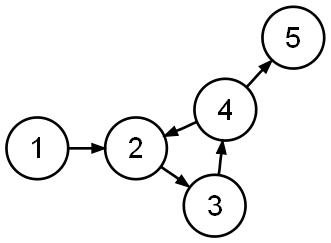
\includegraphics[width=0.40\textwidth]{graph1.png}
	\caption{Directed graph}\label{digraph}
\end{figure}

\begin{figure}[htp]
	\centering
	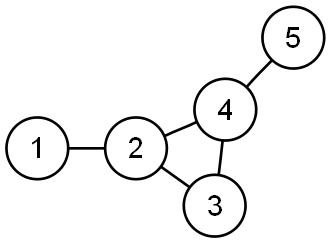
\includegraphics[width=0.40\textwidth]{graph4.png}
	\caption{Undirected graph}\label{undigraph}
\end{figure}

\subsection{Path}
A \textbf{path} on $ G $ is a sequence of vertices such that 
from each of its vertices there is an edge to the next vertex in the sequence. 
i.e. $ \lbrace v_0,v_1,\cdots,v_N \rbrace$ 
such that $ (v_{i-1},v_i) \in A $ for $\forall i \in \left[ 1,N \right]$.
A \textbf{cycle} is a path such that the start vertex and end vertex are the same.
\textbf{N-cycle} is a cycle that has a length N of path such that $ v_0 =v_N $.
If the set of all cycles that have less length than common divider $ k $, 
then that graph is said to be \textbf{k-periodic}. 
\textbf{Acycle} graph is a graph that has no cycle. 
Sometimes, this graph is called \textbf{aperiodic} or \textbf{primitive}.
For aperiodic graph, there is necessarily a vertex 
which has no path from the others or to the others.
A vertex which is not head of any edge is \textbf{initial} or \textbf{follower}, 
and a vertex which is not tail of any edge is \textbf{final} or \textbf{leader}.


\begin{example}[Leader and Follower]
	In figure \ref{digraph}, the vertex 1 is follower, 
	and the vertex 5 is leader.
\end{example}


\subsection{Connectivity}
In an undirected graph $ G $, two vertices $ u $ and $ v $ are called \textbf{connected} 
if G contains a path from $u$ to $v$. 
Otherwise, they are called \textbf{disconnected}.
A directed graph is called \textbf{weakly connected} 
if replacing all of its directed edges with undirected edges 
produces a connected (undirected) graph. (i.e. one way connection)
It is \textbf{strongly connected} if it contains a directed path from $ u $ to $v$ 
for every pair of vertices $u,v \in V$. (i.e. two-way connection)
A graph is \textbf{complete} if every pair of distinct vertices is connected by an edge,
in which each pair of vertices is joined by an edge, 
that is, the graph contains all possible edges.

\begin{figure}[htp]
	\centering
	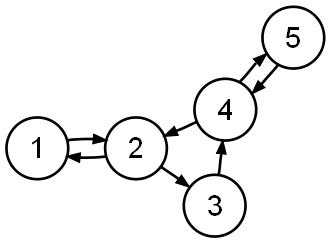
\includegraphics[width=0.40\textwidth]{graph2.png}
	\caption{Strongly connected graph (Irreducible)}\label{stronggraph}
\end{figure}

\begin{example}[Strongly and Weakly Connected]
	The graph in figure \ref{stronggraph} is strongly connected. 
	All vertices are connected to each other.
	The graph in figure \ref{digraph} is weakly connected due to vertices $ 1 $, $ 5 $. 
	The vertex 1 has no path from the others, and the vertex 5 has no path to the others.
\end{example}

\subsection{Component}
For a directed graph, \textbf{components} are its maximal strongly connected subgraphs 
which are said to be strongly connected components(SCC). These form a partition of the graph.
If each strongly connected component is contracted to a single vertex, 
the resulting graph is a directed acyclic graph.
Such as the previous case of the vertex, 
A component in which all vertex is not head of any edge is initial or follower,
and a component in which all vertex is not tail of any edge is final or leader.

\begin{example}[Component]
	In figure \ref{digraph}, there are three components as shown below.
	\begin{enumerate}
		\item A subgraph with vertices $ \lbrace 1 \rbrace $ as follower,
		\item A subgraph with vertices $ \lbrace 2,3,4 \rbrace $,
		\item A subgraph with vertices $ \lbrace 5 \rbrace $ as leader.
	\end{enumerate}
\end{example}

\subsection{Graph Representation}

The \textbf{adjacency matrix} denoted as $ A $ is the representation for a graph.
For given finite graph $ G $ on $ n $ vertices, it is the $ n \times n $ matrix 
where the nondiagonal entry $ a_{ij} $ is the number of edges from vertex $ i $ to vertex $ j $, 
and the diagonal entry $ a_{ii} $ is the number of loops.
If the graph is undirected, the adjacency matrix is symmetric.
The \textbf{normalized adjacency matrix} of a graph on $ n $ vertices is a variation of an adjacency matrix, 
of which the sum of each row entries is normalized to be one. This matrix will be denoted as $ G $.
Now, we introduce the \textbf{Laplacian matrix} denoted as $ L $. 
For a graph without loops from vertex $ i $ to $ i $ or multiple edges from one vertex to another,
the Laplacian matrix is defined as 
$ L = \lbrace l_{ij}  \rbrace$
\begin{equation}\label{laplacian}
l_{ij}=\begin{cases}
1 & \text{ if } i=j \text{ and } d_i \neq 0, \\
-\frac{1}{d_i} & \text{ if } i \neq j \text{ and } \exists edge(i, j), \\
0 & \text{ otherwise.}  \\
\end{cases}
\end{equation} 
for $i,j=1, ..., N$ where $d_i$ is the out-degree of vertex $i$. 
More explanation of the Laplacian matrix is covered in \cite{russell}.

\begin{example}[Graph Representation]
	In Figure \ref{undigraph}, Normalized adjacency matrix $ G $ 
	and Laplacian matrix $ L $ are like that
	\begin{equation}
	G = \left[ \begin{array}{ccccc}
	0 & 1 & 0 & 0 & 0 \\
	\frac{1}{3} & 0 & \frac{1}{3} & \frac{1}{3} & 0 \\
	0 & \frac{1}{2} & 0 & \frac{1}{2} & 0 \\
	0 & \frac{1}{3} & \frac{1}{3} & 0 & \frac{1}{3} \\
	0 & 0 & 0 & 1 & 0 \\ 
	\end{array}  \right] 
	\quad L = \left[ \begin{array}{ccccc}
	1 & -1 & 0 & 0 & 0 \\
	-\frac{1}{3} & 1 & -\frac{1}{3} & -\frac{1}{3} & 0 \\
	0 & -\frac{1}{2} & 1 & -\frac{1}{2} & 0 \\
	0 & -\frac{1}{3} & -\frac{1}{3} & 1 & -\frac{1}{3} \\
	0 & 0 & 0 & -1 & 1 \\ 
	\end{array}  \right] 
	\end{equation}
\end{example}

\begin{remark}	
	\begin{equation}		L= I_n^\star -G	\end{equation}
	\begin{equation}	
		I_n^\star=diag(i_1,\cdots,i_n), \qquad i_j =	
		\begin{cases} 1 & \text{if } d_j > 0,	\\
		0 & \text{otherwise.} \\ \end{cases} 
	\end{equation}		
	Moreover, if all out-degree of vertices is non-zero,
	\begin{equation}
		L= I_n -G
	\end{equation}		
\end{remark}

\begin{theorem}
	The Laplacian matrix $ L \in \R^{n \times n} $ always has 
	the vector $ \ONE_n \triangleq [1, \cdots, 1]^T \in \R^n $ as a member of the null space of $ L $.
	\begin{equation}
	L \ONE_n = 0 
	\end{equation}
\end{theorem}
\begin{proof}
	By multiplication $ \ONE_n $ to a right side of $ L $, we immediately know $ L \ONE_n = 0  $.
\end{proof}


\subsection{Irreducible}

A matrix $ A \in \R^{n \times n} $ is said to be \textbf{reducible} if either
$ n=1 $ and $ A=0 $; or $ n \geq 2$, there is a permutation matrix $ P \in M^{n \times n} $ 
and there is some integer $ r $ with $ 1 \leq r \leq n-1 $ such that
\[ P^T A P =\left[ \begin{array}{cc}
B & C\\ 0 & D \\\end{array} \right] \]
where $ B \in \R^{r \times r},\, D \in \R^{n-r \times n-r},\,C \in \R^{r \times n-r}, $ 
and $ 0 \in \R^{n-r \times r} $ is a zero matrix.
A matrix $ A \in \R^{n \times n} $ is \textbf{irreducible} if it is not reducible.

A directed graph is \textbf{irreducible} if, given any two vertices, 
there exists a path from the first vertex to the second.
A directed graph is irreducible if and only if its Laplacian matrix is irreducible.

\begin{figure}[htp]
	\centering
	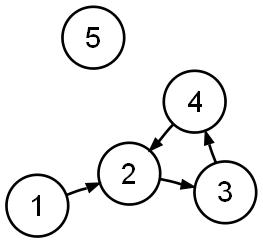
\includegraphics[width=0.32\textwidth]{graph3.png}
	\caption{Reducible graph (Disconnected)}\label{redugraph}
\end{figure}

\begin{theorem}
	A directed graph $ G $ is strongly connected 
	if and only if its adjacency matrix is irreducible.
\end{theorem}
\begin{proof}
	See Theorem 6.2.24 in \cite{horn}.
\end{proof}


\section{Nonnegative Matrix}
From here, we would study nonnegative matrix theory 
and especially we are interested in the relation between the null space of $ L $ and its properties.
Many of materials described here come from \cite{horn}.

\begin{definition}[Nonnegative Matrix and Vector]
	Consider $ A = \lbrace a_{ij} \rbrace \in \R^{n \times m} $.
	If all $ a_{ij} \geq 0 $, then $ A $ is said to be 
	a \textbf{nonnegative matrix} denoted as $ A \geq 0 $.
		
	Similarly, assume that $ v \in \R^{n} $ is a vector of which all elements are nonnegative. 
	$ v $ is called \textbf{nonnegative vector}.
\end{definition}

\begin{definition}[Spectral Radius $ r(A) $]
	The set of all $ \lambda $ that are eigenvalues of $ A \in \C^{n \times n} $ is
	called the spectrum of $ A $ and is denoted by $ \sigma(A) $. The \textbf{spectral radius of $ A $}
	is the nonnegative real number 
	$ r(A) = \max \lbrace \vert \lambda \vert : \lambda \in \sigma(A) \rbrace $.
	This is just the radius of the smallest disc centered at the origin in the complex plane
	that includes all the eigenvalues of $ A $.
\end{definition}

\begin{theorem}\label{spectralineq}
	If $ \Vert \cdot \Vert $ is any matrix norm, then
	\begin{equation}
		r(A) \leq \Vert A \Vert, \qquad A \in \C^{n \times n} 	
	\end{equation}
\end{theorem}
\begin{proof}% Theorem 5.6.9 in \cite{horn}
	Assume that $ \vert \lambda \vert= r(A) $ and $ X $ is all the columns of which are
	equal to the eigenvector $ x $ such that $ Ax=\lambda x$, $ x \neq 0 $.	
	\[ \vert \lambda \vert \Vert X \Vert =  \Vert \lambda X \Vert  
		= \Vert AX \Vert \leq \Vert A \Vert	\Vert X \Vert 
		\Rightarrow r(A) \leq \Vert A \Vert \]	
\end{proof}

\begin{theorem}[Perron-Frobenius Theorem for Nonnegative Irreducible Matrices]\label{perron}
	Let $ A \in \C^{n \times n} $ and suppose that $ A $ is irreducible and nonnegative. Then
	\begin{enumerate}
		\item $ r(A) > 0 $.
		\item $ r(A) $ is an eigenvalue of A.
		\item There is a positive vector $ x $ such that $ Ax = r(A)x $.
		\item $ r(A) $ is an algebraically simple eigenvalue\footnote
		{An algebraically simple eigenvalue has the algebraic multiplicity which is equal to $ 1 $.}
		 of $ A $.
	\end{enumerate}
\end{theorem}

\begin{proof}
	See Theorem 8.4.4 in \cite{horn}.
\end{proof}

\begin{remark}
	Assume that $ A $ has $ r(A) $ as the spectral radius, then $ A^T $ has also.
	Moreover, if $ A $ is irreducible and nonnegative, then $ A^T $ is so, and
	it is also true that there is a positive vector $ y $ such that $ A^Ty =r(A)y $
	as well as a positive vector $ x $ such that $ Ax=r(A)x $.
\end{remark}

\begin{definition}[Stochastic Matrix]
	Consider a $ n \times n $ matrix $ A $.
    The matrix $ A $ is said to be a \textbf{row stochastic matrix} 
		if each of whose rows consists of nonnegative real numbers with 
		each row summing to $ 1 $.
    Analogously, it is a \textbf{column stochastic matrix} if 
	whose columns consist of nonnegative real numbers whose sum is $ 1 $.
    And a \textbf{doubly stochastic matrix} if the matrix $ A $ 
	is a row and column stochastic matrix.
\end{definition}

\begin{remark}
	The normalized adjacency matrix $ G $ is a stochastic one.
\end{remark}

\begin{theorem}\label{sdisk}
	The spectrum of a stochastic matrix is contained in the unit circle in the complex plane.	
\end{theorem}
\begin{proof}
	Assume the matrix $ A $ is stochastic.
	We can easily prove the theorem by investigating the norm of a stochastic matix $ A $ 
	with the property $ r(A) \leq \Vert A \Vert $ of Theorem \ref{spectralineq}.	
	If $ A $ is row stochastic, 
		$ \left\Vert A\right\Vert _\infty 
		= \max_i \left(\sum_j \left\vert a_{ij}\right\vert\right)=1 $
		which is the maximum row sum,
	and if $ A $ is column stochastic,
		$ \left\Vert A\right\Vert _1 		
		= \max_j \left(\sum_i \left\vert a_{ij}\right\vert\right)=1 $
		which is the maximum column sum.
\end{proof}

\begin{theorem}\label{poseigenv}
	Assume that $ r = r(G) $
	where $ G \in \R^{n \times n} $ is a normalized adjacency matrix.
	If $ G $ is irreducible or its directed graph is strongly connected, then 
	there exist positive vectors $ x,y^T \in \R^n $ 
	such that $ Gx=r x $ and $ G^T y = r y$.
	Moreover, $ r $ is an algebraically simple eigenvalue of $ G $, 
	and $ r $ is $ 1 $.
\end{theorem}

\begin{proof}
	Because of the normalized adjacency matrix's property that $ G \ONE_n = 1 \ONE_n $, 
	we have the eigenvalue $ 1 $ corresponding the eigenvector $ \ONE_n $ of $ G $.
	By Theorem \ref{sdisk}, $ 1 $ is the largest one of eigenvalues of $ G $. 
	Thus, $ r =1 $.	
	
	Now, under the given assumption that $ G $ is irreducible and nonnegative.	
	By Theorem \ref{perron}, we straightforwardly have positive vectors $ x, y^T $
	such that $ Gx=x $ and $ G^T y=y $, 
	and the eigenvalue $ r=1 $ of G has the multiplicity $ 1 $.
\end{proof}

\begin{theorem}\label{nullspan}
	Assume that $ L \in \R^{n \times n}$ is the Laplacian matrix of a directed graph 
	which is strongly connected.
	The left and right null space of $ L $ are 
	individually spanned by a single positive vector.
\end{theorem}

\begin{proof}	
	At first, we claim that 
	an eigenvalue $ \lambda $ of $ L $ corresponds to $ 1-\lambda $	of $ G $.
	By virtue of strongly connected graph, there is no vertex which has $ 0 $ as its out-degree.
	Thus, $ L=I_n -G $. Assume that $ v $ is the eigenvector of $ L $ associated with $ \lambda $.
	\begin{equation}
		Lv= (I_n-G)v=\lambda v \quad \Leftrightarrow \quad Gv=(1-\lambda)v
	\end{equation}
	Therefore, an eigenvalue $ \lambda_i(L) $ of L is defined as
	\begin{equation}
		\lambda_i(L) = 1 - \lambda_i(G)
	\end{equation}
	where $ \lambda_i(G) $ is an eigenvalues of $ G $ and $ i \in [1,n] $.
	Moreover, the matrices $ G $ and $ L $ share the same eigenvectors.

	Now, we already know that $ G $ has $ r(G)=1 $ which is simple,
	and corresponding left and right eigenvectors
	$ x, y^T $ such that $ Gx=1x $ and $ G^T y=1y $ are positive via Theorem \ref{poseigenv}.
	Hence, $ L $ has $ 1-r(G)=0 $ as a simple eigenvalue  and $ Lx=0x=0, L^Ty=0y=0 $.
	Consequently, the left and right null space of $ L $ are spanned by a single positive vector. 	
\end{proof}	

\begin{theorem}\label{singleleader}
	Assume that $ L \in \R^{n \times n}$ is the Laplacian matrix of a directed graph 
	which has a single leader component.
	The left null space of $ L $ includes a nonnegative vector except the zero.
\end{theorem}

\begin{proof}
	When $ L $ has a single leader component,
	we can write the normalized adjacency matrix $ G = I_n - L $
	as follows with a permutation matrix $ P $.
	\begin{equation}
		P G P^T = \left[ \begin{array}{cccc} G_{11} & 0 & \cdots & 0 \\
		G_{21} & G_{22} & 0 & 0 \\
		\vdots &  & \ddots & \vdots \\
		G_{m1} & G_{m2} & \cdots & G_{mm} \\	\end{array} \right]	
	\end{equation}
	where $ G_{ii} $ are irreducible which stand for strong connected components,
	and $ m $ is the number of components of the graph represented by $ G $.
	Now, consider $ G_{11} $. In the same manner of Theorem \ref{nullspan},
	there is a vector $ y $ which spans the left nullspace of $ I-G_{11} $
	, that is $ y(I-G_{11}) =0 $. If we choose $ y^\star \in \R^{1 \times n} $ such that 
	$ y^\star =\left[ y,0,\cdots,0 \right]  $, then,
	\begin{equation}\begin{split}
	y^\star (I_n -PGP^T) &= y^\star ( PP^T -PGP^T)=y^\star P (I_n-G)P^T =0	\\
	&\Rightarrow y^* L =0, \qquad y^* = y^\star P \\
	\end{split}\end{equation}
	As a result, we have the nonnegative vector $ y^* $ included in the left nullspace of $ L $.
	% When a graph has a single leader component, 
	% assume that a leader component has only one vertex which is $ i $-th vertex.
	% If one eliminates the $ i $-th row and $ i $-th column from the laplacian matrix $ L $
	% corresponding to $ i $-th vertex as the leader,
	% we know that the submatrix $ S $ of its laplician matrix $ L $ is an irreducible matrix
	% that means its subgraph is strongly connected.
	% In a similar manner of Theorem \ref{nullspan}, 
	% there exists the positive vectors $ x_s $ and $ y_s^T $
	% such that $ Sx_s=0 $, $ S^Ty_s=0 $.
	% And in that case, we can choose 
	% the vector $ x=P^{-1}\left[1,  x_s\right]^T  $ spanning the right nullspace of $ L $, and
	% the vector $ y^T=P^{-1}\left[y_1, y_s^T\right]^T  $ spanning the left nullspace of $ L $
	% where $ P $ is the permutation matrix 
	% which places $ i $-th element to $ 1 $-st one of a vector
	% while preserving the order of other vertices, 
	% and $ y_1 = - y_s l_{ri} $ 
	% when $ l_{ri} $ is the column vector 
	% from the $ i $-th column of $ L $ without the $ i$-th element.
\end{proof}

	
Before closing this section, we additionally introduce a result about the relation 
among the dimension of nullspace of $ L $, the number of leader components 
and nonnegative vectors from \cite{faxthesis} and \cite{roth}. 

\begin{theorem}
	The multiplicity $ m $ of the zero eigenvalue of the Laplacian matrix $ L $ is 
	equal to the number of leader components of its graph. The dimension of the nullspace of $ L $
	is also equal to $ m $, and is spanned by a basis of $ m $ nonnegative vectors.
\end{theorem}

\begin{proof}See Proposition 4.5 in \cite{faxthesis}.\end{proof}

\begin{remark}
	If a graph has multiple leader components, 
	then the the dimension of the nullspace of its Laplacian matrix 
	%may not be greater than $ 1 $.
	might be greater than $ 1 $.
\end{remark}


\section{Control Analysis and Design}

Now, we consider systems \eqref{brusys} over again. 
One can put the systems of $ N $ agents into one single system together 
by the Kronecker product and the Laplacian matrix.
If we set the weight $ w_{ij} $ of system \eqref{brusys} 
to $ \frac{1}{\vert \NBR_i \vert} $\footnote
{$ \vert \NBR_i \vert $ is the cardinality of $ \NBR_i $, 
that is the number of agents which the agent $ i $ can sense.}, 
then we have a very simple form of \eqref{newout} 
together by virtue of the Laplacian matrix as the next theorem.
See \cite{fax} as a consensus algorithm\footnote{The consensus problem is 
to have a group of agents reach a common assessment based on distributed information.} 
in cooperative control.

Before proceeding our analysis, we would redefine $ \frac{a}{\vert A \vert } $
as $ 0 $ if $ \vert A \vert =0 $,
to avoid the division by $ 0 $ where $ A $ and $ a $ are arbitrary set and number.
This definition does not conflict with a conventional inverse of a number in our theorem.


\begin{theorem}\label{laplacianform}
	For the following collection of multiple homogeneous systems,
	\begin{equation}\begin{split}
	\dot{z_i}&=Az_i+Bv_i, \\
	y_i & =\sum_{j \in \NBR_i}w_{ij}(Cz_i-Cz_j),  \\
	& A \in \R^{n \times n},\quad B \in \R^{n \times m}, 
	\quad C \in \R^{m \times n}, \quad w_{ij} \in \R  \\
	\end{split}\end{equation} 
	for $ 1 \leq \forall i \leq N $ 
	where $  \NBR_i \subset [1,N] \setminus \lbrace i \rbrace $ 
	is an index set that represents the set of agents which agent $ i $ can sense.
	If
	\begin{equation}\label{weightcond}
	w_{ij} = \frac{1}{\vert \NBR_i \vert},
	\end{equation}
	then the above collection of systems can be rewritten as one system
	\begin{equation}\begin{split}
	\dot{z} &= A_N z + B_N v, \\
	y &= L_{(m)} C_N z \\
	\end{split}\end{equation}
	where
	\begin{equation}\begin{split}\label{whereterms}
	z &= \left[ z_1,z_2,\cdots,z_N \right] ^T, \\
	v &= \left[ v_1,v_2,\cdots,v_N \right] ^T, \quad
	y = \left[ y_1,y_2,\cdots,y_N \right] ^T, \\
	A_N & = I_N \otimes A, \quad B_N  = I_N \otimes B, \quad C_N  = I_N \otimes C,\\
	L_{(m)} & = L \otimes I_m, \quad L=\lbrace l_{ij} \rbrace  \in \R^{N \times N}, \\
	l_{ij}&=\begin{cases}
	1 & \text{ if } i=j,  \\
	-\frac{1}{\vert \NBR_i \vert} & \text{ if } i \neq j \text{ and } j \in \NBR_i , \\
	0 & \text{ otherwise.}  \\
	\end{cases}\\
	\end{split}\end{equation}
\end{theorem}

\begin{proof}
	Straightforwardly, the collection of $ z_i $ can be written as follows
	\begin{equation}\begin{split}
	\left[ \begin{array}{c} \dot{z_1} \\ \dot{z_2} \\  \vdots \\ \dot{z_N} \end{array}  \right] &=
	\left[ \begin{array}{cccc} A & 0 & \cdots & 0\\
	0 & A & \cdots & 0 \\
	0 & 0 & \ddots & 0 \\
	0 & 0 & \cdots & A \\
	  \end{array} \right]
	\left[ \begin{array}{c} z_1 \\ z_2 \\  \vdots \\ z_N \end{array}  \right] 
	+
	\left[ \begin{array}{cccc} B & 0 & \cdots & 0\\
	0 & B & \cdots & 0 \\
	0 & 0 & \ddots & 0 \\
	0 & 0 & \cdots & B \\
	  \end{array} \right]
	\left[ \begin{array}{c} v_1 \\ v_2 \\  \vdots \\ v_N \end{array}  \right]  \\
	&= (I_N \otimes A) z + (I_N \otimes B) v= A_N z + B_N v =\dot{z}  \\
	\end{split}\end{equation}

	Next, we now investigate the collection of $ y_i $.
	Let $ G \in \R^{N \times N}$ be the matrix as shown below. 
	Note that $ G $ is a normalized adjacency matrix.
	\begin{equation}\begin{split}\label{matrixg}
	G&=diag(\frac{1}{\vert \NBR_1 \vert},\frac{1}{\vert \NBR_2 \vert}  ,\cdots, 
	\frac{1}{\vert \NBR_N \vert} ) 
	\left[ \begin{array}{cccc} g_{11} & g_{12} & \cdots & g_{1N} \\
	g_{21} & g_{22} & \cdots & g_{2N} \\
	\vdots &  & \ddots & \vdots \\
	g_{N1} & g_{N2} & \cdots & g_{NN} \\ \end{array} \right] \\	
	& \qquad\qquad\qquad g_{ij} = \begin{cases}
	1 & \text{if } i \neq j \text{ and } j \in \NBR_i ,\\
	0 & \text{otherwise.}\\
	\end{cases} \\
	& \qquad\qquad\qquad G_i = \text{the $i$-th row of G} \\	
	\end{split}\end{equation}
		
	\begin{equation}\begin{split}
	y_i & =\sum_{j \in \NBR_i}w_{ij}(Cz_i-Cz_j)
	=\sum_{j \in \NBR_i}\frac{1}{\vert \NBR_i \vert}(Cz_i-Cz_j) \\
	&=\frac{1}{\vert \NBR_i \vert}\sum_{j \in \NBR_i}(Cz_i-Cz_j) 
	=\frac{1}{\vert \NBR_i \vert} ( \vert \NBR_i \vert Cz_i - \sum_{j \in \NBR_i}Cz_j )  \\
	&=Cz_i - \frac{1}{\vert \NBR_i \vert} \sum_{j \in \NBR_i}Cz_j \\
	&=Cz_i - \frac{1}{\vert \NBR_i \vert} (\left[ g_{i1}, g_{i2},\cdots, g_{iN} \right] \otimes I_m)
	\left[ \begin{array}{c} Cz_1 \\ Cz_2 \\ \vdots \\ Cz_N \end{array}  \right] \\
	%\left[Cz_1, Cz_2, \cdots, Cz_N \right]^T  \\
	&=Cz_i - (\frac{1}{\vert \NBR_i \vert} \left[ g_{i1}, g_{i2},\cdots, g_{iN} \right] \otimes I_m)
	(I_N \otimes C)z \\
	&=Cz_i - (G_i \otimes I_m)(I_N \otimes C)z \\
	\end{split}\end{equation}	
	Thus, the collection of $ y_i $ is to be such that
	\begin{equation}\begin{split}
	\left[ \begin{array}{c} y_1 \\ y_2 \\  \vdots \\ y_N \end{array}  \right] &=
	\left[ \begin{array}{cccc} C & 0 & \cdots & 0\\
	0 & C & \cdots & 0 \\
	0 & 0 & \ddots & 0 \\
	0 & 0 & \cdots & C \\
	  \end{array} \right]
	\left[ \begin{array}{c} z_1 \\ z_2 \\  \vdots \\ z_N \end{array}  \right] \\
	& \quad - \left[ \begin{array}{cccc} G_1 \otimes I_m  & 0 & \cdots & 0\\
	0 & G_2 \otimes I_m & \cdots & 0 \\
	0 & 0 & \ddots & 0 \\
	0 & 0 & \cdots & G_N \otimes I_m   \\
	  \end{array} \right]  
	\left[ \begin{array}{cccc} C & 0 & \cdots & 0\\
	0 & C & \cdots & 0 \\
	0 & 0 & \ddots & 0 \\
	0 & 0 & \cdots & C \\
	  \end{array} \right]
	\left[ \begin{array}{c} z_1 \\ z_2 \\  \vdots \\ z_N \end{array}  \right] \\
	&=(I_N \otimes C)z - (G \otimes I_m)(I_N \otimes C)z \\
	&=(I_{Nm} - G \otimes I_m)(I_N \otimes C)z \\
	&=((I_{N} - G) \otimes I_m)(I_N \otimes C)z \\
	&=(L \otimes I_m)(I_N \otimes C)z \\
	&=L_{(m)}C_N z = y \\
	\end{split}\end{equation}
\end{proof}

\begin{corollary}
	For the collection of input-output feedback linearized systems 
	of homogeneous agents \eqref{brusys}, If 
	\begin{equation}
	w_{ij} = \frac{1}{\vert \NBR_i \vert},
	\end{equation}
	then they can be simplified to 
	\begin{equation}\begin{split}\label{multicollection}
	\dot{\xi} &= \phi(\xi,z,v), \\
	\dot{z} &= A_N z + B_N v, \\
	y^* &= L_{(m)} C_N z \\
	\end{split}\end{equation}
	where $ y^* = \left[ y_1^*, \cdots, y_N^* \right]^T$, 
	$ A_N, B_N, C_N, L_{(m)} $ are such that equations \eqref{whereterms} 	
	in Theorem \ref{laplacianform}.	
\end{corollary}

\begin{theorem}\label{multireltracking}
	Consider system \eqref{multicollection}, 
	Assume that the tracking dynamics of the agent are bounded input bounded state stable,
	$ y_{(ij)r} \in \R^m $ are the relative references\footnote
	{$( Cz_i(t) - Cz_j(t)) \to y_{(ij)r}(t) $ as $ t \to \infty $.}
	of \eqref{defreltrack},
	and $ \lambda(L) $ is the set of eigenvalues of $ L $.	\\	
	Choose $ y_{ir} $ such that
	\begin{equation}
	y_{(ij)r} = y_{ir} - y_{jr}
	\qquad \text{ for }  1 \leq \forall i,j \leq N.
	\end{equation}	If 
	\begin{equation}\label{multihurwitz}
	\begin{array}{c} 
	s^{\rho_1} + \lambda_i k_{1\rho_1} s^{\rho_1-1} + \cdots + \lambda_i k_{11}, \\
	\vdots \\
	s^{\rho_m} + \lambda_i k_{m\rho_m} s^{\rho_m-1} + \cdots + \lambda_i k_{m1} \\
	\end{array}
	\end{equation} 
	are Hurwitz polynomials for 
	$ \forall \lambda_i \in \lambda(L) $ such that $ \lambda_i \neq 0 $,	
	and the multiplicity of the eigenvalue $ \lambda_i $ such that $ \lambda_i = 0$
	is\footnote{The dimension of nullspace of $ L $.} $ 1 $, 	
	furthermore, 
	a nonnegative vector except the zero is included in the left null space of $ L $,
	then
	%and the left null space of $ L $ is spanned by a single nonnegative vector\footnote
	%{The vector is said to be \textbf{nonnegative} 
	%if all its elements are greater than or equal to 0. } 	$ \in \R^{1 \times N} $ except the zero, 
	%
	%and the multiplicity of the eigenvalue $ \lambda_i $ such that $ \lambda_i = 0$\footnote
	%{The dimension of nullspace of L.} is $ 1 $, then 
	\begin{equation}\label{trackingstmt}
	\lim_{t \to \infty} y^* (t) = y_{r}^* (t) 
	\end{equation}
	with the controller 
	$ v=\left[ v_{11},\cdots,v_{1m}, \cdots\cdots,v_{N1},\cdots,v_{Nm} \right]^T $ as follows
	\begin{equation}\begin{split}\label{decontrol}
	v_{i1}& = -k_{11}(y_{i1}^* - y_{i1r}^* (t) ) - \cdots 
	- k_{1\rho_1} ({y_{i1}^*}^{(\rho_1 -1)} - {y_{i1r}^*}^{(\rho_1 -1)} (t) ) + {y_{i1r}}^{(\rho_1)} (t) \\
	&\qquad\qquad\qquad\qquad\qquad\qquad\qquad \vdots \\
	v_{im}& = -k_{m1}(y_{im}^* - y_{imr}^* (t) ) - \cdots 
	- k_{m\rho_m} ({y_{im}^*}^{(\rho_1 -1)} - {y_{imr}^*}^{(\rho_m -1)} (t) ) + {y_{imr}}^{(\rho_m)} (t) \\
	\end{split}\end{equation} 	
	where 	
	\begin{equation}\begin{split}			
	y_r &= \left[ y_{1r}, y_{2r}, \cdots, y_{Nr} \right]^T, \\
	y_r^* &= L_{(m)}y_r, \\
	y_{ijr}^* &\text{ is the } ( (i-1) \times m + j)\text{-th element of } y_r^* ,\\
	y_{ij}^* &\text{ is the } ( (i-1) \times m + j)\text{-th element of } y^* \\	
	\end{split}\end{equation}
\end{theorem}

\begin{proof}
	We can prove the above theorem in a similar manner with the proof of Theorem \ref{trackingthm}.

	For each $ j \in \left[ 1,m \right] $, 
	Let $ e_{ijk} \triangleq {y_{ij}^*}^{(k-1)}-{y_{ijr}^*}^{(k-1)} $. 
	One can then take $ v_i =\left[ v_{i1}, \cdots, v_{im} \right]^T $ as the equation \eqref{decontrol}. 
	We obtain		
	\begin{equation*}\begin{split}
	\dot{e}_{ijk} &= e_{ij(k+1)} , \qquad 1\leq k \leq \rho_{j-1}, \\
	\dot{e}_{ij\rho_j} &= {y_{ij}^*}^{(\rho_j)}-{y_{ijr}^*}^{(\rho_j)} \\
	&=  \frac{1}{\Vert \NBR_i \Vert } \sum_{l \in \NBR_i}( \dot{z_{ij\rho_j}} - \dot{z_{lj\rho_j}})	
	   -\frac{1}{\Vert \NBR_i \Vert } \sum_{l \in \NBR_i}({y_{ijr}}^{(\rho_j)} - {y_{ljr}}^{(\rho_j)}) \\	
	&=  \frac{1}{\Vert \NBR_i \Vert } \sum_{l \in \NBR_i}
		( v_{ij} - v_{lj} - {y_{ijr}}^{(\rho_j)} + {y_{ljr}}^{(\rho_j)} ) \\		
	&=  \frac{1}{\Vert \NBR_i \Vert } \sum_{l \in \NBR_i}
		( (v_{ij} - {y_{ijr}}^{(\rho_j)})- (v_{lj}  - {y_{ljr}}^{(\rho_j)}) ) \\			
	&=  (v_{ij} - {y_{ijr}}^{(\rho_j)} )
		-\frac{1}{\Vert \NBR_i \Vert } \sum_{l \in \NBR_i} (v_{lj}  - {y_{ljr}}^{(\rho_j)}) \\
	&= -k_{j1}(y_{ij}^* - y_{ijr}^* ) - \cdots - k_{j\rho_j} ({y_{ij}^*}^{(\rho_1 -1)} 
		- {y_{ijr}^*}^{(\rho_j -1)}) + {y_{ijr}}^{(\rho_j)}  -{y_{ijr}}^{(\rho_j)}  \\
		&\qquad -\frac{1}{\Vert \NBR_i \Vert } \sum_{l \in \NBR_i} 
		(-k_{j1}(y_{lj}^* - y_{ljr}^* ) - \cdots - k_{j\rho_j} ({y_{lj}^*}^{(\rho_1 -1)} 	
		- {y_{ljr}^*}^{(\rho_j -1)}) 
		\\ &\qquad\qquad \qquad\qquad + {y_{ljr}}^{(\rho_j)}  -{y_{ljr}}^{(\rho_j)} ) \\
	&= -k_{j1} e_{ij1} - \cdots - k_{j\rho_j} e_{ij\rho_j} 
		-\frac{1}{\Vert \NBR_i \Vert } \sum_{l \in \NBR_i} 
		(-k_{j1} e_{lj1} - \cdots - k_{j\rho_j} e_{lj\rho_j} ) \\
	\end{split}\end{equation*}		
	for $1 \leq \forall i \leq N$. Thus, as a simple form,
	\begin{equation}\begin{split}
		\dot{e}_{ij} 
		&= H_j e_{ij} -\frac{1}{\Vert \NBR_i \Vert } \sum_{l \in \NBR_i} F_j H_j e_{ij} \\
		&= H_j e_{ij} - F_j H_j (G_i \otimes I_{\rho_j}) e_{j}
		\qquad\qquad 1 \leq \forall j \leq m \\
	\end{split}\end{equation}	
	where
	\begin{equation}\begin{split}	
		H_j &=\left[\begin{array}{cccc}
		0 & 1 & \cdots & 0\\
		\vdots & \vdots & \ddots & \vdots\\
		0 & 0 & \cdots & 1\\
		-k_{j1} & -k_{j2} & \cdots & -k_{j\rho_j}\end{array}\right],
		\quad
		F_j = \left[\begin{array}{cccc}
		0 & 0 & \cdots & 1\\
		\vdots & \vdots & \ddots & \vdots\\
		0 & 0 & \cdots & 1\\
		0 & 0 & \cdots & 1\end{array}\right] \in \R^{\rho_j \times \rho_j}, \\		
		e_{ij} &= \left[ 
		\begin{array}{c } e_{ij1} \\ \vdots \\  e_{ij\rho_j-1} \\ e_{ij\rho_j} \\ \end{array}	 
		\right],
		\quad		
		e_{j} = \left[ 
		\begin{array}{c } e_{1j} \\ \vdots \\  e_{N-1j} \\ e_{Nj} \\ \end{array}	 
		\right],
		\quad
		G_i \text{ is that as \eqref{matrixg} }
	\end{split}\end{equation}		
	Then, we have the collection $ e_{j} $ of $ e_{ij} $,  $ \forall i \in \left[ 1,N \right] $,
	as shown below.	
	\begin{equation}\begin{split}\label{errdynamics}
	\dot{e_j} &= (I_N \otimes H_j) e_j - (I_N \otimes F_j H_j)(G \otimes I_{\rho_j}) e_j \\
	&= (I_N \otimes H_j) e_j  - (G \otimes F_j H_j ) e_j \\
	&= (I_N \otimes H_j) e_j  - (G \otimes F_j )(I_N \otimes H_j ) e_j \\
	&= (I_{N\rho_j}-G \otimes F_j )(I_N \otimes H_j ) e_j  \\
	&= (I_N \otimes I_{\rho_j} -G \otimes F_j )(I_N \otimes H_j ) e_j  \\
	&= (I_N \otimes I_{\rho_j} +(I_N-G) \otimes F_j  - I_N \otimes F_j )(I_N \otimes H_j ) e_j  \\
	&= (I_N \otimes (I_{\rho_j} -F_j ) +L \otimes F_j  )(I_N \otimes H_j ) e_j  \\
	&= ( (L \otimes F_j )(I_N \otimes H_j ) + I_N \otimes (H_j -F_j H_j ) ) e_j\\	
	&= ( L \otimes F_j H_j  + I_N \otimes N_j  ) e_j \\	
	\end{split}\end{equation}
	where
	\begin{equation}
	N_j  = \left[ \begin{array}{cccc } 
		0 & 1 & \cdots & 0\\
		\vdots & \vdots & \ddots & \vdots\\
		0 & 0 & \cdots & 1\\
		0 & 0 & \cdots & 0	
		\end{array} \right] % = H_j -F_j H_j 
	\end{equation}
	
	From now, we want to know the asymptoticity of the matrix 
	$ E_j  \triangleq L \otimes F_j H_j  + I_N \otimes N_j  $.
	If one can transform $ E_j $ into an upper triangular form via similarity transformation
	which preserves the stability of an given system,
	we are easily able to check a stability of the system \eqref{errdynamics}.	
	If the error dynamics \eqref{errdynamics} of output tracking by relative references 
	is asymptotically stable, the statement \eqref{trackingstmt} is true.
	
	By Schur's unitary\footnote{A matrix $ T \in \C^{n \times n} $ is said to be \textbf{unitary}
	if $ T^H T=I $. In addition, $ T \in \R^{n \times n} $ is said to be \textbf{real orthogonal}. }
	triangularization theorem\cite{horn}, 
	we can choose a real orthogonal matrix $ T $ such that $ U=T^{-1}LT $ 
	in which, $ U $ is an upper triangular matrix, 
	and	the diagonal entries of $ U $ are exactly the eigenvalues of $ L $.
	
	By the similarity transformation $ \tilde{e_j}=(T^{-1} \otimes I_{\rho_j}) e_j$, 
	we will get an upper triangular system like this,
	which has the same stability property with system \eqref{errdynamics}.
	\begin{equation}\begin{split}\label{similarform}	
		\dot{\tilde{e_j}} &= (T^{-1} \otimes I_{\rho_j}) 
			( L \otimes F_j H_j  + I_N \otimes N_j  ) 
			(T \otimes I_{\rho_j}) \tilde{e_j} \\
		&= 	( T^{-1} L T \otimes F_j H_j  + I_N \otimes N_j  ) \tilde{e_j} \\
		&= 	( U \otimes F_j H_j  + I_N \otimes N_j  ) \tilde{e_j} \\
	\end{split}\end{equation}	
	Let
	\begin{equation}\begin{split}		
	H_{j\lambda} = \lambda F_j H_j  +N_j  = \left[\begin{array}{cccc}
		0 & 1 & \cdots & 0\\
		\vdots & \vdots & \ddots & \vdots\\
		0 & 0 & \cdots & 1\\
		-\lambda k_{j1} & -\lambda k_{j2} & \cdots & -\lambda k_{j\rho_j}\end{array}\right] \\
	\end{split}\end{equation}
	The characteristic equation of system \eqref{similarform} is 
	%i.e. $ det( (U \otimes F_j H_j  + I_N \otimes N_j )  - sI_{N_\rho_j}) $, is
	\begin{equation}\begin{split}\label{cheq}
		\prod_{\lambda_i \in \lambda(L)}  det(H_{j\lambda_i} -sI_{\rho_j} )
		&= \prod_{\lambda_i \in \lambda(L)} 
		s^{\rho_j} + \lambda_i k_{j\rho_j} s^{\rho_j-1} + \cdots + \lambda_i k_{j1} \\	
	\end{split}\end{equation}
	by the benefit from an upper triangular shape.
	
	For our assumption \eqref{multihurwitz}, 
	All roots $ s $ of the characteristic equation \eqref{cheq} 
	have negative real parts except $ s=0 $ when $ \lambda_i=0 $. 
	Therefore, at least, system \eqref{similarform} is stable 
	and system \eqref{errdynamics} is as well by the similarity.
	If one has no invariant points except $ {e_j} =0 $ when $ s=0 $,
	we may say that system \eqref{errdynamics} is asymptotic stable 
	by Lasalle's invariance principle\cite{khalil}.
	
	At this time, we will find the invariant points of system \eqref{errdynamics}
	by setting $ \dot{e}_j = 0 $.
	We know the dimension of the null space of $ L \otimes F_j H_j  + I_N \otimes N_j  $
	is $ 1 $ by the assumption,	
	%\footnote{In assumptions, 
	%The left null space of $ L $ is spanned by a \textbf{single} nonnegative vector,
	%and $ L $ always have the vector $ \ONE_N $ as a member of (right) null space by its property.}
	and propose the vector 
	$ \ONE_N \otimes \left[ 1, 0, \cdots ,0 \right]^T $
	as the basis of the null space. That is easily checked by substitution.
	Thus, $ e_j $ can be represented as follows.	
	\begin{equation}\label{invariant}
	e_j=c (\ONE_N \otimes \left[ 1, 0, \cdots ,0 \right]^T)
	\end{equation}
	where $ c \in \R $. In the above equation, 
	if it is the only possible case of $ c $  that $ c= 0 $, 
	the invariant points of system \eqref{errdynamics} is the origin $ e_j = 0 $.
	
	Now, assume that $ c $ is non-zero. 
	One can get non-zero elements from \eqref{invariant} as shown below.
	\begin{equation}
	\left[ \begin{array}{c}	e_{1j1} \\	e_{2j1} \\	\vdots  \\	e_{Nj1} \\	\end{array} \right] = 
	\left[ \begin{array}{c}	y_{1j}^* - y_{1jr}^* \\	y_{2j}^* - y_{2jr}^* \\	
		\vdots  \\	y_{Nj}^* - y_{Njr}^* \\	\end{array} \right] 
	= L (I_N \otimes O_j) (y-y_{r}) = c \ONE_N 
	\end{equation}
	where
	\begin{equation}
		O_j = \lbrace o_{1k} \rbrace,
		\qquad k \in \left[1,m\right],
		\qquad o_{1k} = \begin{cases} 1 & k=j \\ 0 & otherwise. \end{cases}		
	\end{equation}
	% \begin{equation}
	% \left[ \begin{array}{c}	e_{1j1} \\	e_{2j1} \\	\vdots  \\	e_{Nj1} \\	\end{array} \right] = 
	% \left[ \begin{array}{c}	y_{1}^* - y_{1r}^* \\	y_{2}^* - y_{2r}^* \\	
		% \vdots  \\	y_{N}^* - y_{Nr}^* \\	\end{array} \right] 
	% = L (y-y_r) = c \ONE_N 
	% \end{equation}
	% If we multiply a non-zero vector from the left null space of L,
	If we multiply a nonnegative vector of our assumption to both sides, 
	which is included in the left null space of $ L $,
	$ c $ should be zero by contradiction.
	\begin{equation}
	n_l L (I_N \otimes O_j)(y-y_r) = n_l c \ONE_N \neq 0, 
	\quad \text{Nonnegative } n_l \in \text{Left Null Space of }L
	\end{equation}
	Consequently, $ e_j $ asymptotically approaches the origin.
	Because we have an asymptotic stable system for every $ j \in \left[ 1, m\right] $,
	one can finally attain that $ y^* \to {y_{r}}^* $ as $ t \to \infty $.

	Since $ y^* $ are bounded, it follows that $ z(t) $ are bounded.
	By the property of the bounded input bounded state stability of the tracking dynamics, 
	$ \xi (t)  $ from \eqref{multicollection} is bounded as well, $ z(t) $
	as bounded references.
\end{proof}
	
Now, we should ensure that, if
\[ \lim_{t \to \infty} y^* (t) = y_{r}^* (t) \]
then 
\[ \lim_{t \to \infty} \Vert ( Cz_i(t) - Cz_j(t)) - y_{(ij)r}(t) \Vert =0 \]
that is our goal of output tracking by relative references.

\begin{theorem}
	Consider system \eqref{multicollection} 
	under the condition of Theorem \ref{multireltracking}. If
	\begin{equation}
		\lim_{t \to \infty} y^* (t) = y_{r}^* (t),
	\end{equation}
	then
	\begin{equation}
		\lim_{t \to \infty} \Vert ( Cz_i(t) - Cz_j(t)) - y_{(ij)r}(t) \Vert =0
	\end{equation}
\end{theorem}

\begin{proof}
	\begin{equation}\begin{split}
	y^* - y_{r}^* &= L_{(m)}(y-y_r)=0 \\
	& \Downarrow \quad \because \text{The null space of $ L $ is spanned by } \ONE_N \\
	y_i-y_{ir} = c \ONE_{m} \quad &\Leftrightarrow \quad y_i = y_{ir}  + c\ONE_{m} \\
	& \Downarrow \\
	Cz_i - Cz_j = y_i -y_j &= y_{ir} +c\ONE_{m} -y_{jr} -c\ONE_{m} =  y_{ir} -y_{jr}  =y_{(ij)r} \\
	\end{split}\end{equation}
\end{proof}


\begin{corollary}\label{corosol}
	For system \eqref{multicollection},
	if it satisfies the condition of Theorem \ref{multireltracking}, then
	the problem of the output tracking by relative references is solvable.
\end{corollary}

\begin{remark}[Strongly Connected and Single Leader Component]\label{scslremark}
	If the directed graph of the Laplacian matrix $ L $ is strongly connected or
	has a single leader component, 
	then the left null space of $ L $ includes  
	a nonnegative vector and its dimension is $ 1 $ 
	through Theorem \ref{nullspan} and \ref{singleleader}.	
	Thus, we can replace 
	the condition of a nonnegative vector included in the left null space of $ L $
	and the nullity 1 of $ L $ with the property of strongly connected graph 
	or a single leader component for the Laplacian matrix $ L $.
\end{remark}

\begin{remark}
	The controller $ v_i $ in equation \eqref{decontrol} is a decentralized one\footnote
	{The decentralized controller depends on only neighbors of each agents, not all agents.}. 
	In the $ i $-th agent, we have the controller $ v_i $ as follows.
	\begin{equation}
		v_i = -\frac{1}{\vert \NBR_i \vert} \sum_{l \in M}
				K_{l}  \sum_{j \in \NBR_i } (y_i - y_j - y_{ir}(t) + y_{jr}(t)) ^{(l-1)}  
				+ \left[  \begin{array}{c } y_{i1r}^{(\rho_1)}(t) \\
				\vdots \\	y_{imr}^{(\rho_m)}(t) \end{array}	   \right] \\
	\end{equation} 	
	where
	\begin{equation}\begin{split}
		M &= \lbrace 1,2,\cdots, max(\rho_1,\cdots,\rho_m) \rbrace \\
		K_l &= \left[  \begin{array}{cccc } 
		k_{1l}^\star & 0 & \cdots & 0 \\
		0 & k_{2l}^\star & & 0 \\
		\vdots & & \ddots & \vdots \\
		0 & 0 & \cdots & k_{ml}^\star \\
		\end{array} \right] ,
		% \left[ \begin{array}{c } k_{1l}^\star \\		\vdots \\		
		% k_{ml}^\star \\		\end{array} \right], 
		\qquad 
		k_{jl}^\star = \begin{cases} k_{jl} & \text{if } l \leq \rho_j, \\	0 & otherwise. \\
		\end{cases}	\\
	\end{split}\end{equation}
	
	Thus, for the collection of systems \eqref{multisys}, 
	we have the feedback controller $ u_i $ with $ v_i $ of the $ i $-th agent
	for the tracking problem as shown below.
	\begin{equation}\begin{split}\label{ctrlui}
		u_i 
		% &= -\A^{-1}(x_i)
		% \left[ \begin{array}{c}L_f^{\rho_1} h_1\\ L_f^{\rho_2} h_2\\ \vdots\\ 
		% L_f^{\rho_m} h_m\end{array} \right] + \A^{-1}(x_i)v_i \\
		&= -\A^{-1}(x_i) \left( L_f^\rho h(x_i)			
		    - \left( \frac{1}{\vert \NBR_i \vert} \sum_{l \in M}
				K_{l}  \sum_{j \in \NBR_i } (y_i - y_j -  y_{ir} + y_{jr}) ^{(l-1)}  
				+  y_{ir}^{(\rho)}(t) \right)\right)\\			
	\end{split}\end{equation} 	
	where
	\begin{equation}\begin{split}
		L_f^\rho h(x_i) &= \left[ 
		\begin{array}{c } L_f^{\rho_1}h_1(x_i) \\ \vdots \\ L_f^{\rho_m}h_m(x_i) \end{array} \right],
		% \left[ \begin{array}{c}L_f^{\rho_1} h_1\\ L_f^{\rho_2} h_2\\ \vdots\\ 
		% 	L_f^{\rho_m} h_m\end{array} \right],
		\qquad y_{ir}^{(\rho)}(t) = \left[  \begin{array}{c } y_{i1r}^{(\rho_1)} (t) \\
				\vdots \\	y_{imr}^{(\rho_m)} (t) \end{array}	   \right], \\
		\A (x_i)&=\left[\begin{array}{ccc}
		L_{g_1} L_f^{\rho_1 -1} h_1 (x_i) & \cdots & L_{g_m} L_f^{\rho_1 -1} h_1 (x_i)\\
		L_{g_1} L_f^{\rho_2 -1} h_2 (x_i) & \cdots & L_{g_m} L_f^{\rho_2 -1} h_2 (x_i)\\
		\vdots & \ddots & \vdots\\
		L_{g_1} L_f^{\rho_m -1} h_m (x_i) & \cdots & L_{g_m} L_f^{\rho_m -1} h_m (x_i)\\\end{array}\right] \\
	\end{split}\end{equation}
\end{remark}	

In this chapter, we have considered the collection of multiple homogeneous systems \eqref{multisys}.	
When the global vector relative degree $ \rho $ is well defined 
with $ \rho^* \leq n $, the vector fields \eqref{vfield} are complete, 
and the references for systems \eqref{multisys} are given by relative values.
If the output of each agent system can be absolutely measurable by itself, then
we can transform each agent system into the system \eqref{brusys} 
via input-output feedback linearization.

For given relative references, one can set new output form of the system \eqref{brusys},
and with the assumption of scalars for weights like \eqref{weightcond}, 
we can rewrite the collection of systems as one big system \eqref{multicollection} 
by the Laplacian matrix $ L $ and the Kronecker product.

If the directed graph of the Laplacian matrix $ L $ is strongly connected or
has a single leader component, then the left null space of $ L $ includes at least 
one nonnegative vector except the zero, and its dimension is $ 1 $. Therefore, 
under assumption that the tracking dynamics of the agent is bounded input bounded output stable,
we can finally have a tracking controller $ u_i $ subject to the condition \eqref{multihurwitz}.
Moreover, $ u_i $ is represented by the equation \eqref{ctrlui} as shown above.


\chapter{Formation Tracking Control}

% 쉽게 쉽게 쓰자.....
% 얼른 쓰고 쉬고 싶어. 
% 이번 chapter의 목표는 1주일
% Take it easy!!!
% 2008.3.17

This chapter is composed of two parts about the formation tracking problem and
the permutation invariant formation tracking problem.
Before we discuss the formation tracking control, the common concept of formations is described. 
And the formation is mathematically defined as the matrix and the vector 
about relative outputs of the agents in the group.

\begin{figure}[htp]
	% \centering
	% 
\includegraphics[width=0.40\textwidth]{t50flight.png}
	% \caption{Patrolling flight of T-50, Republic of Korea Air Force}
	% \end{figure}
	\centering
	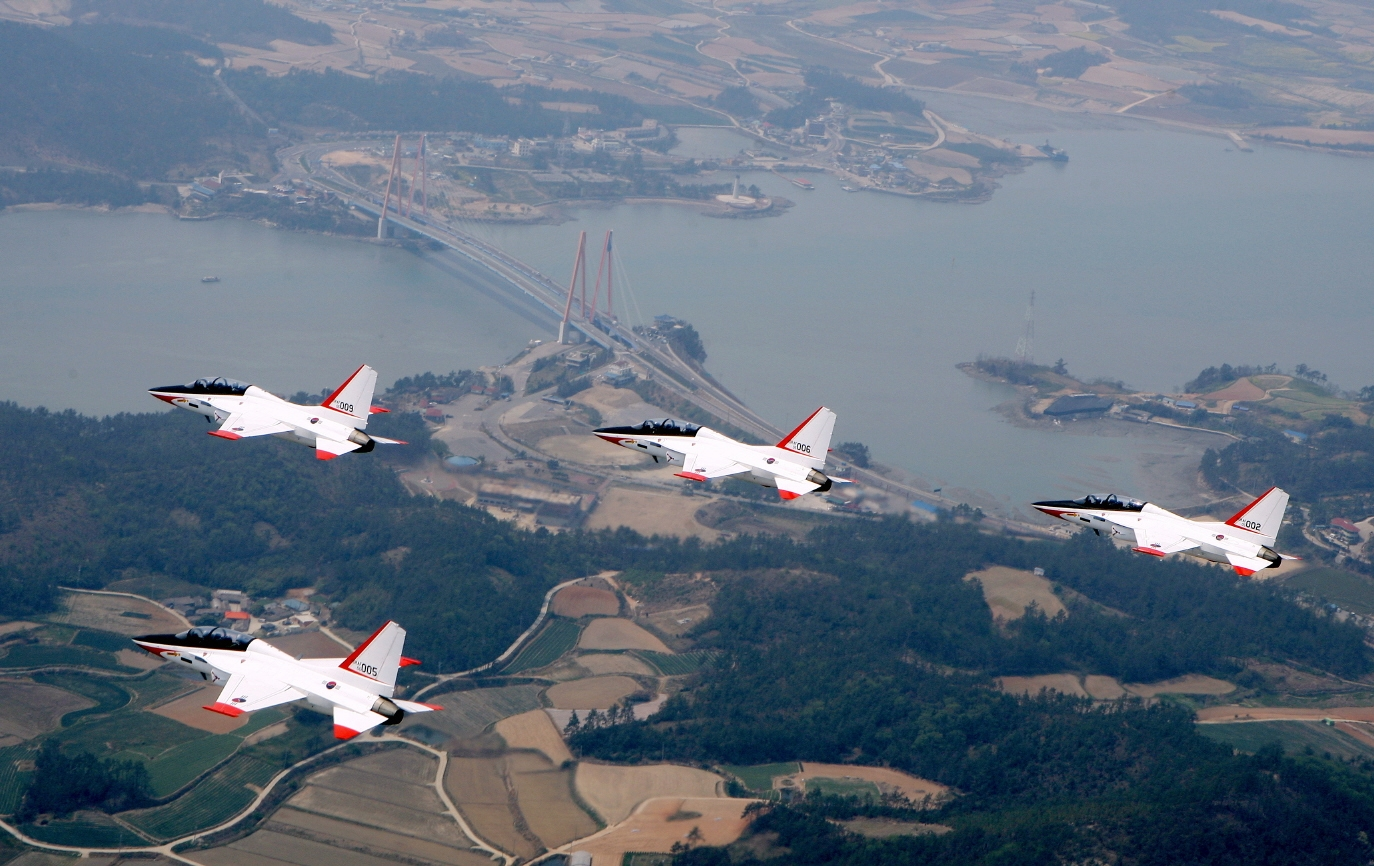
\includegraphics[width=0.80\textwidth]{t50flight2.jpg}
	\caption{Patrolling flight of T-50, Republic of Korea Air Force.}
\end{figure}

\section{Formation}

In this section, we describe what formation is, and mathematically define it.
The term of formation is used in a variety of areas. 
In military, a formation means the physical deployment of moving military forces 
like ground forces, aircrafts, and sea vessels. 
Examples of a formation includes line, square, V form and so on, 
that is the arrangement for tactical mission.

In sports, 
for instance, in football,
the formation illustrates how the players in a team are positioned on a playground.
Various formation can be used relying on more defensive or offensive playing 
by which a team might be characterized.
\begin{figure}[htp]
	\centering
	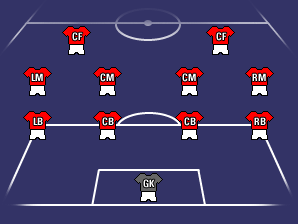
\includegraphics[width=0.60\textwidth]{football.png}
	\caption{4-4-2 Formation, sometimes called a flat-back 4. 
	The midfielders are required to work hard to support both the defence and the attack.
	Courtesy of Eteamz.com}
\end{figure}

Concerning transportation system, formation can be considered as platooning of vehicles.
Figure \ref{platoon} shows the platooning of cars on a highway. 
Through formation control,
one can achieve to grow the capacity of highway and to enhance the safety 
without additional lanes and equipments
by decreasing the space between cars and increasing the density of traffic.
\begin{figure}[htp]
	\centering
	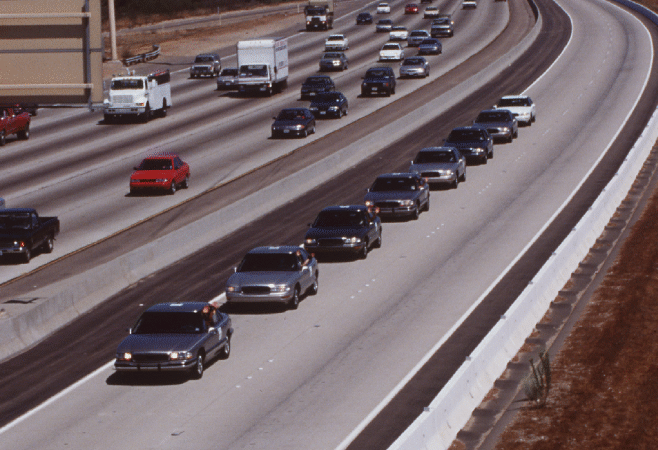
\includegraphics[width=0.70\textwidth]{platoon.png}
	\caption{The platoon control demonstration in San Diego 
	by the National Automated Highway System Consortium. See \cite{path}.}
	\label{platoon}
\end{figure}

Generally speaking, Formation commonly indicates a configuration of some agents
in the sense of position or location while aiming to coordinate a shared operation among agents.
In such formation, each agent is able to freely move to all direction. 
Hence, formation should not include an absolute location.
Thus, it would be a relative information between the states of the agents.
Now, we mathematically define the formation to explain a formation control that is our issue.

\subsection{Formation Matrix}

\begin{definition}[Formation Matrix F]
	For the collection of $ N $ agents, each agent $ i $ has the states $ y_i \in \R^m$
	that represent a quantity of position or motional traits as its output.
	\textbf{Formation Matrix} $ F $ is a $ mN \times N $ matrix of smooth vector fields
	with respect to time as follows.
	\begin{equation}\begin{split}\label{fmatrix}
		F(t) &= \left[ \begin{array}{ccc} f_{11}(t) & \cdots & f_{1N}(t) \\
		\vdots & \ddots & \vdots \\
		f_{N1}(t) & \cdots & f_{NN}(t) \\ 	\end{array} \right], \quad f_{ij}(\cdot) \in \R^m , \\
		f_{ij}(t) &= f_{ik}(t) - f_{jk}(t), \quad 
		%f_{ii}(t)=\left[ 0, \cdots, 0 \right]^T,  \\
		\quad 1 \leq \forall k \leq N
		%, \quad i \neq j  \\
	\end{split}\end{equation}
\end{definition}

\begin{remark}
	The condition $ f_{ij}(t) = f_{ik}(t) - f_{jk}(t) $ of \eqref{fmatrix} describes 
	the feasibility of a shape. For instance, in a triangle, 
	the largest edge of the triangle should be shorter than the sum of other edges.
	Otherwise, the three edges can not make a triangle.
	See \cite{feasible} about the feasibility of the formation.
\end{remark}

\begin{remark}
	If a formation matrix $ F $ contains a $ f_{ij} $, 
	then the $ -f_{ij} $ is also included in $ F $.	
	Moreover, $ f_{ij} = -f_{ji} $. ($ \because f_{ij} = f_{ii}-f_{ji} = -f_{ji} $)
\end{remark}
% \begin{remark}{Existence}
	% $ f_{ij} $ complete어쩌구 하는 것은 실제로 가능한 formation을 위한 것
	% existence
% \end{remark}
% \begin{remark}{Uniqueness}
	% F는 여러개일까??
% \end{remark}

\begin{figure}[htp]
	\centering
	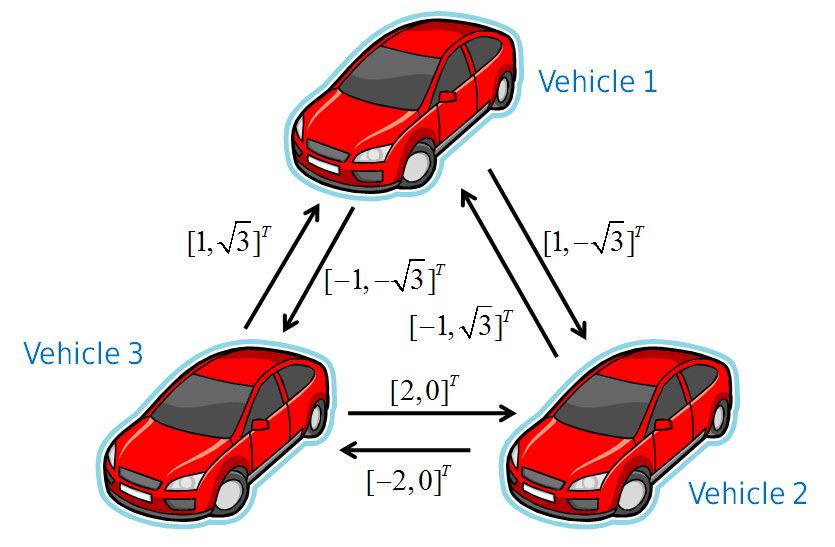
\includegraphics[width=0.70\textwidth]{triangle.png}
	\caption{The three vehicles in the equilateral triangle formation 
			with $ 2 $-dimensional relative outputs.}
	\label{trivehicles}
\end{figure}

\begin{example}[Formation Matrix]
	In Figure \ref{trivehicles}, the formation matrix $ F $ is defined as shown below.
	\begin{equation}\label{exfmatrix}
		F = \left[ \begin{array}{ccc } 
		0 & -1 & 1 \\
		0 & \sqrt{3} & \sqrt{3} \\
		1 & 0 & 2 \\
		-\sqrt{3} & 0 & 0 \\
		-1 & -2 & 0 \\
		-\sqrt{3} & 0 & 0 \\
		\end{array} \right]
	\end{equation}
\end{example}

\subsection{Formation of Agents}

\begin{definition}[Formation]
	Consider the collection of $ N $ agents. 
	Assume that each agent $ i $ has the states $ y_i \in \R^m $ 
	that represent a quantity of position or motional traits as its output.
	The collection of $ N $ agents are \textbf{in the formation $ F $}
	if $ y_i - y_j = f_{ij}(t) $ for $ 1 \leq \forall i,j \leq N $
	where $ f_{ij}(\cdot) \in \R^m $ is the submatrix   
	of the $ mN \times N $ formation matrix $ F $ like \eqref{fmatrix}.
\end{definition}

\begin{remark}
	In the formation $ F $, the group of agents can freely move anywhere.
	Information of a formation does not have an absolute value on the outputs of the agents.
\end{remark}


\subsection{Formation Vector}

\begin{definition}[Formation Vector $\zeta$]
	For a $ mN \times N $ formation matrix $ F $,
	\textbf{Formation vector} $ \zeta $ is a $ mN $-dimensional smooth vector field as shown below.
	\begin{equation}\label{fvec}
		F = \zeta \otimes \ONE_{N}^T   - \ONE_{N} \otimes \zeta^{\dag}
	\end{equation}	
	where 
	\begin{equation}\begin{split}\label{fvector}
		%\ONE_{mn} &= \left[ \begin{array}{cccc } 1 & 1 & \cdots & 1 \\
		%\vdots &  & \ddots & \vdots \\
		%1 & 1 & \cdots & 1 \\		
		%\end{array} \right] \in \R^{m \times n}, 
		%\quad		
		\zeta &= \left[ \relbar \zeta_1^T \relbar,\cdots,\relbar \zeta_N^T \relbar \right]^T \in \R^{mN}, \\
		\zeta^{\dag} &= \left[ \begin{array}{ccc } \vert & & \vert \\
		\zeta_1 & \cdots &\zeta_N \\	\vert & & \vert \\
		\end{array} \right] \in \R^{m \times N}, \\
		\zeta_i(\cdot) &= \left[ \zeta_{i1}(\cdot), \cdots , \zeta_{im}(\cdot)  \right]^T \in \R^m \\		
	\end{split}\end{equation}
\end{definition}

\begin{remark}
	If the dimension of the output $ m $ is $ 1 $, the formation vector $ \zeta $ satisfies
	\begin{equation}
		F = \zeta  \ONE_{N}^T   - \ONE_{N} \zeta^{T}
	\end{equation}
\end{remark}

\begin{remark}
	For the given formation matrix $ F $ and formation vector $ \zeta $ in the above definition,
	\begin{equation}
		f_{ij}(t) = \zeta_i(t) - \zeta_j(t)
	\end{equation}
	where $ f_{ij} $, $ \zeta_i $ are defined as \eqref{fmatrix} and \eqref{fvector}.
\end{remark}

\begin{remark}
	For the equation \eqref{fvec},
	there are many formation vectors that satisfies the condition.
	One can easily choose a formation vector $ \zeta $ 
	by setting $ \zeta_i $ to the difference 
	between an arbitrary constant vector $ h \in \R^m $ and $ y_i $ 
	when the agents are in the formation.\cite{faxthesis}
	\begin{equation}
		\zeta_i = y_i - h
	\end{equation}
\end{remark}

\begin{example}\label{exfvector}
	For the formation matrix $ F $ in \eqref{exfmatrix} corresponding Figure \ref{trivehicles}, 
	a following vector $ \zeta $ is the formation vector.	
	\begin{equation}\begin{split}
		F &= \zeta \otimes \ONE_{3}^T   - \ONE_{3} \otimes \zeta^{\dag}, \\
		\zeta&=\left[ 0,0,1,-\sqrt{3},-1,-\sqrt{3} \right]^T, \quad 
		\zeta^\dag = \left[  \begin{array}{c c c } 
		0 & 1 & -1 \\
		0 & -\sqrt{3} & -\sqrt{3} \\
		\end{array}\right]\\		
	\end{split}\end{equation}
\end{example}


\section{Formation Tracking}

Consider the collection of multiple systems.
\begin{equation}\begin{split}\label{formationsys}
	\dot{x_1} &=f_1(x_1)+g_1(x_1)u_1, \qquad\qquad  y_1 = h_1(x_1), \\
	\dot{x_2} &=f_2(x_2)+g_2(x_2)u_2, \qquad\qquad  y_2 = h_2(x_2),\\
	& \qquad \qquad \vdots \\
	\dot{x_N} &=f_N(x_N)+g_N(x_N)u_N, \qquad\quad  y_N = h_N(x_N),\\
\end{split}\end{equation} 
where
\begin{alignat*}{3}
	u_i&=\left[u_{i1} ,\cdots ,u_{im}\right]^T ,  \qquad & u_i & \in \R^m \\
	%g(x)&=\left[g_1 (x) ,\cdots ,g_m (x) \right]   \qquad & g(x) & \in \R^{n \times m} \\
	g_i(x_i)&=\left[ \begin{array}{ccc}
	\vert & & \vert \\
	g_{i1} (x_i), & \cdots , & g_{im} (x_i) \\
	\vert & & \vert \\
	\end{array} \right],   \qquad & g_i(\cdot) & \in \R^{n \times m} \\
	h_i(x_i)&=\left[h_{i1} (x_i) ,\cdots ,h_{im} (x_i) \right]^T , \qquad & h_i(\cdot) & \in \R^m  
\end{alignat*} 
with $ x_i \in \R^n $ $ (1 \leq \forall i \leq N) $,  
smooth $ f_i $ and $ g_{i1} ,\cdots g_{im} $ vector fields over $\R^n$ 
and $ h_{ij} $: $\R^n \rightarrow \R$ 
a smooth function s.t. $ h_{ij}(0)=0 \quad (0 \leq \forall j \leq m) $. 

\begin{definition}[Formation Tracking Problem]
	For the collection of multiple systems \eqref{formationsys},
	the \textbf{formation tracking problem} is to design a controller with the property that,
	for a formation matrix $ F $ like \eqref{fmatrix},
	the outputs of systems satisfies
	\begin{equation}
		\lim_{t \to \infty}\Vert \left(y_i(t) - y_j(t) \right) - f_{ij}(t) \Vert = 0, 
		\qquad 1\ \leq \forall i,j \leq N 	
	\end{equation}
	for any initial condition of the closed loop system. Therefore, 
	the collection of multiple systems would be in the formation $ F $ by the controller.
\end{definition}

\begin{remark}
	For a formation tracking problem, 
	One can think about the rotation of the group in the formation.
	But, the formation matrix changes under the rotation.
	Actually, a formation matrix is invariant 
	under the translation of the group but not under the its rotation.
	One might deal with such a rotation invariant formation 
	with introducing a rotation matrix where we will not consider the case.	
\end{remark}

\begin{remark}
	For a formation tracking problem, 
	one can replace the formation matrix $ F $ 
	with a formation vector $ \zeta $ like \eqref{fvec}	as follows.
	\begin{equation}
		\lim_{t \to \infty}\Vert \left(y_i(t) - y_j(t) \right)
		-\left( \zeta_i(t) - \zeta_j(t) \right) \Vert = 0, 
		\qquad 1\ \leq \forall i,j \leq N 	
	\end{equation}	
\end{remark}

\begin{remark}
	For the collection of the system \eqref{formationsys},
	if $ f_i $, $ g_i $ and $ h_i $ are respectively identical for $ 1 \leq \forall i \leq N $, 
	then we can deal with a formation tracking problem as
	an output tracking of multiple homogeneous agents by relative references.
	In that case, relative references are to be $ f_{ij} $ of a formation matrix $ F $.
\end{remark}

\begin{theorem}[Formation Tracking Control]\label{formationcontrolthm}
	Consider the collection of the agent systems \eqref{formationsys}. 	
	Assume that $ f_i $, $ g_i $ and $ h_i $ are respectively identical 
	for $ 1 \leq \forall i \leq N $	that means homogeneous systems,
	and	the Laplacian matrix $ L $ stands for an output sensing graph $ \GRP $ of the agents
	in which each agent $ i $ can sense the outputs of its neighbors $ \NBR_i $.
	For a formation vector $ \zeta $ like \eqref{fvector},
	if \begin{itemize}
		\item 	the agent is globally state feedback input-output linearizable,
		\item	each output of agents is absolutely measurable by itself, 		
		\item	the tracking dynamics of the agent is bounded input bounded state stable,
		\item	the directed graph $ \GRP $ of the Laplacian $ L $ is 
				strongly connected or has a single leader component,
		\item	and $ s^{\rho_j} + \lambda_i k_{j\rho_j} s^{\rho_j-1} + \cdots + \lambda_i k_{j1} $ 
				are Hurwitz polynomials for $ \forall \lambda_i \in \lambda(L) $ 
				such that $ \lambda_i \neq 0 $, $ 1 \leq \forall j \leq m $,
	\end{itemize}
	then, the formation tracking problem is solvable with the controller $ u_i $ as shown below.
	\begin{equation}\begin{split}
		u_i &= -\A^{-1}(x_i) \left( L_f^\rho h(x_i)			
		    - \left( \frac{1}{\vert \NBR_i \vert} \sum_{l \in M}
				K_{l}  \sum_{j \in \NBR_i } (y_i - y_j -  \zeta_{i} + \zeta_{j}) ^{(l-1)}  
				+  \zeta_{i}^{(\rho)}(t) \right)\right)\\			
	\end{split}\end{equation} 	
	where
	\begin{equation}\begin{split}\label{trackingthmwhere}
		\rho &=\left[ \rho_1,\cdots,\rho_m \right]^T \in \N^{m} 
		\text{ as the vector relative degree of the agent},\\
		M &= \lbrace 1,2,\cdots, max(\rho_1,\cdots,\rho_m) \rbrace, \\		
		K_l &= \left[  \begin{array}{cccc } 
		k_{1l}^\star & 0 & \cdots & 0 \\
		0 & k_{2l}^\star & & 0 \\
		\vdots & & \ddots & \vdots \\
		0 & 0 & \cdots & k_{ml}^\star \\
		\end{array} \right] ,
		% \left[ \begin{array}{c } k_{1l}^\star \\		\vdots \\		
		% k_{ml}^\star \\		\end{array} \right], 
		\qquad 		
		k_{jl}^\star = \begin{cases} k_{jl} & \text{if } l \leq \rho_j, \\	0 & otherwise. \\		\end{cases}	\\			
		L_f^\rho h(x_i) &= \left[ 
		\begin{array}{c } L_f^{\rho_1}h_1(x_i) \\ \vdots \\ L_f^{\rho_m}h_m(x_i) \end{array} \right], 
		\qquad\qquad
		\zeta_{i}^{(\rho)}(t) = \left[  \begin{array}{c } \zeta_{i1}^{(\rho_1)} (t) \\
			\vdots \\	\zeta_{im}^{(\rho_m)} (t) \end{array}	   \right], \\			
		\A (x_i) &=\left[\begin{array}{ccc}
		L_{g_1} L_f^{\rho_1 -1} h_1 (x_i) & \cdots & L_{g_m} L_f^{\rho_1 -1} h_1 (x_i)\\
		L_{g_1} L_f^{\rho_2 -1} h_2 (x_i) & \cdots & L_{g_m} L_f^{\rho_2 -1} h_2 (x_i)\\
		\vdots & \ddots & \vdots\\
		L_{g_1} L_f^{\rho_m -1} h_m (x_i) & \cdots & L_{g_m} L_f^{\rho_m -1} h_m (x_i)\\\end{array}\right] \\
	\end{split}\end{equation}
\end{theorem}

\begin{proof}
	If we respectively choose $ \zeta_i $ and $ \zeta_j $ as $ y_{ir} $ and $ y_{jr} $
	in Theorem \ref{multireltracking},
	then, one can straightforwardly prove the given theorem.
	See	Theorem \ref{brusysthm}, \ref{nullspan}, \ref{singleleader}, \ref{multireltracking}
	and Corollary \ref{corosol}.
\end{proof}

\section{Permutation of Agents}

In this section, we think about an permutation of the agents in the formation.
Consider the collection of multiple homogeneous agents. 
Each of agents is identical to the others
which means that every agents have the same ability of not only the movement
but also the other features in the group.
In the formation, a certain agent can equivalently play a role 
even though its position might be changed. 
This concept is one that the formation is unchanged 
by permuting the agents in the group,
which is described by the term of permutation invariant formation in \cite{kloder}.

\begin{definition}[Permutation Invariant Formation]\label{piformation}
	Consider the collection of $ N $ agents. 
	Assume that each agent $ i $ has the states $ y_i \in \R^m $ 
	that represent a quantity of position or motional traits as its output.
	The collection of $ N $ agents are \textbf{in the permutation invariant formation $ F $}
	if there exists a bijective function\footnote
	{A bijective function is one-to-one and onto between the domain and range.}
	$ p: A \rightarrow A $ such that
	\begin{equation}\begin{split}\label{pimapping}
		y_{p(i)} - y_{p(j)} &= f_{ij}(t), \qquad		1 \leq \forall i,j \leq N, \\
		A &= \lbrace 1,2,\cdots,N \rbrace \subset \N
	\end{split}\end{equation}
	where $ f_{ij}(\cdot) \in \R^m $ is the submatrix   
	of the $ mN \times N $ formation matrix $ F $ like \eqref{fvector}.	
\end{definition}

\begin{definition}[Formation Assignment and Virtual Agent]
	For the equation \eqref{pimapping}, 
	the function $ p $ does the \textbf{formation assignment on $ F $}
	for the \textbf{virtual agent} in the formation $ F $.
	One might be aware of the mapping $ p $ from $ i $ to $ p(i) $ as 
	the assignment from the $ i $-th virtual agent to the $ p(i) $-th actual agent.
\end{definition}

\begin{remark}
	A bijective function $ p $ in Definition \ref{piformation} can be rewritten 
	by a $ N \times N $ permutation matrix $ P $ 
	and a formation vector $ \zeta $ as shown below.
	\begin{equation}
		y = \left( P \otimes I_m \right) \zeta
	\end{equation}
	where $ y = \left[ y_1,y_2,\cdots,y_N \right]^T $.
\end{remark}

\begin{definition}[Permutation Invariant Formation Tracking Problem]
	Consider the collection of multiple systems \eqref{formationsys} 
	for a formation matrix $ F $ like \eqref{fmatrix}.
	Assume that $ f_i, g_i $ and $ h_i $ are respectively identical 
	for $ 1 \leq \forall i \leq N $, and 
	every agent can equivalently play each role of the agents
	regardless of the index of the agent.
	The \textbf{permutation invariant formation tracking problem} is 
	to design a controller with the property that,	
	the outputs of systems satisfies
	\begin{equation}
		\lim_{t \to \infty}\Vert \left(y_{p(i)}(t) - y_{p(j)}(t) \right) - f_{ij}(t) \Vert = 0, 
		\qquad 1\ \leq \forall i,j \leq N 	
	\end{equation}
	for any initial condition of the closed loop system
	where the function $ p $ is bijective from $ \left[ 1,N \right] $ to $ \left[ 1,N \right] $
	which does the formation assignment on $ F $.
	Therefore, the collection of multiple systems would be 
	in the permutation invariant formation $ F $ by the controller.
\end{definition}

\begin{remark}
	Concerning a permutation invariant formation tracking problem,
	the position of an agent in the formation is not deterministic in the stage of 
	designing the formation matrix.	
	That means that one does not explicitly know 
	which agent in the group goes where in the formation.
\end{remark}

\section{Permutation Invariant Formation Tracking}\label{permutationinvariantformation}

This section is devoted to the discussion of 
how to solve a permutation invariant formation tracking problem. 
In that problem, The permutation matrix $ P $ representing a formation assignment 
is essential to characterize the feature of the formation tracking.
Now, we focus on a configuration of $ P $ to minimize the distance 
for reaching the permutation invariant formation 
in the aspect of the weighted graph matching problem.

\subsection{Weighted Graph Matching Problem}

The weighted graph matching problem is to find a permutation of vertices of one graph such that 
the rearranged vertices make the distance minimized from the edge weights.
Graph match problem is a fundamental one that arises in a lot of fields 
like distributed control, computer vision and facility allocation.
Graph matching problem in this section is that the collection of multiple homogeneous agents
reach a permutation invariant formation while minimizing the distance to getting the formation.

\begin{definition}[Weighted Graph Matching Problem]
	Consider two weighted undirected graphs $ \GRP_1 $ and $ \GRP_2 $ with the same $ n $ vertices.
	Assume that $ A_1 $ and $ A_2 $ are respectively $ n \times n $ weighted adjacency matrices 
	of the graph $ \GRP_1 $ and $ \GRP_2 $.
	The \textbf{weighted graph matching problem} is defined 
	to find the permutation matrix $ P $ such that
	\begin{equation}\label{matchingdef}
		\min_{P \in P_n}  \Vert A_1 - P^T A_2 P \Vert
	\end{equation}
	where $ P_n $ denote the set of all $ n \times n $ permutation matrices, and
	$ \Vert \cdot \Vert $ is a matrix norm.
\end{definition}

\begin{remark}
	If a permutation matrix $ P $ makes the value of \eqref{matchingdef}
	equal to $ 0 $, the two graphs $ \GRP_1 $ and $ \GRP_2 $ have the same structure
	with simple relabelling of the vertices. In such case, we say that the two graphs are 
	\textbf{isomorphic}.
\end{remark}

\begin{figure}[htp]
	\centering
	\subfigure[Graph $ \GRP_1 $]{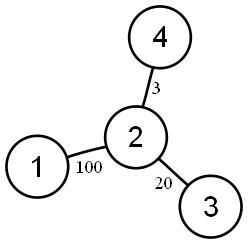
\includegraphics[width=0.35\textwidth]{match1.png}}
	\hspace{7mm}
	\subfigure[Graph $ \GRP_2 $]{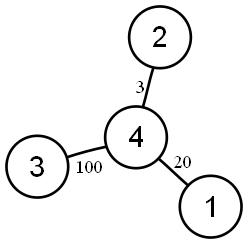
\includegraphics[width=0.35\textwidth]{match2.png}}
	\caption{The graph $ \GRP_1 $ and $ \GRP_2 $ are isomorphic
	while sharing the same structure. By the permutation of the vertices, 
	two graphs come to be identical.}	
	\label{g1g2fig}
\end{figure}


\subsection{Dynamical Approach to Formation Assignment}
Generally, a weighted graph matching problem is known as NP-complete\footnote
{The complexity NP-complete is a subset of NP 
which is the set of non-deterministic polynomial time problems.
A decision problem $ C $ is NP-complete if $ C $ is in NP, and every problem in NP is reducible to $ C $.}. 
See \cite{npc1, npc2}.
It has received a lot of attention due to its hardness. Thus, there are many solutions to tackle
this problem. Now, we introduce one method to solve the weighted graph matching problem.
That is the dynamical system approach which is described in \cite{graphmatch}.
They utilize Theorems of \cite{broc} that is 
about the dynamical systems to sort lists, diagonalize matrices, 
and solve linear programming problems.
This approach has the solution as the trajectory of the system which is dynamically evaluated.
Hence, we can take the advantage of not only the final exact solution of the problem
but also the transient and approximated solution 
that will be used to our problem, the permutation invariant formation tracking 
by rearrangement of the formation vector, later on.

\subsubsection{Dynamical Formation Assignment}
In the paper \cite{graphmatch}, they reformulate the graph matching problem as follows
\begin{equation}\label{matchcost}
	\min_{P \in O_n \cap N_n}  \Vert PA_1 - A_2 P \Vert_F^2	
\end{equation} 
where $ O_n $ denotes the set of $ n \times n $ orthogonal matrices,
$ N_n $ denotes the set of $ n \times n $ element-wise nonnegative matrices, 
and $ \Vert \cdot \Vert_F $ is the Frobenius norm\footnote
{The Frobenius norm is defined as
 $ \Vert A \Vert_F = tr(A A^T)^{\frac{1}{2}}$ for $ X \in \R^{n \times n} $.}
of matrix. 
They claim $ P_n $ is equivalent to $ O_n \cap N_n $, and
construct the dynamical system on the manifold of orthogonal matrices.
That dynamical system has two gradient flows. 
The first one minimizes the cost of weighted graph matching \eqref{matchcost}
and the second one forces the matrix $ P $ to be a permutation matrix
which is the subset of orthogonal matrices.


\begin{theorem}\label{pdynamicsthm}
	Assume that $ A_1 $ and $ A_2 $ are the adjacency matrices
	corresponding to the weighted undirected graphs $ \GRP_1 $ and $ \GRP_2 $, and $ P(0) \in O_n $.
	If $ P(t) $ is the solution of the following matrix differential equation
	\begin{equation}\label{pdynamics}
		\dot{P} = P \left( P^T A_2 P A_1 - A_1 P^T A_2 P \right)
					-k P \left( (P \circ P)^T P -P^T (P \circ P) \right)
	\end{equation}
	for all $ t \geq 0 $ where $ k $ is a positive constant
	and $ A \circ  B $ denotes the element-wise product of the matrices\footnote
	{Suppose that $ A=\lbrace a_{ij} \rbrace $ and $ B=\lbrace b_{ij} \rbrace $.
	Then, $ A \circ  B = \lbrace a_{ij}b_{ij} \rbrace$.}.	
	Then, for sufficiently large $ k $,
	$ lim_{t \to \infty}P(t) = P_\infty $ exists and
	approximates a permutation matrix that also minimizes the distance
	$ \Vert PA_1 - A_2 P \Vert_F^2 $.
	Moreover, the larger $ k $ yields the better $ P_\infty $ that approximates a permutation matrix.
\end{theorem}

\begin{proof}
	See Theorem 3.9 in \cite{graphmatch}.
\end{proof}

\begin{example}
	In Figure \ref{g1g2fig}, 
	the adjacency matrices $ A_1 $ and $ A_2 $ corresponding the graphs $ \GRP_1 $ and $ \GRP_2 $ 
	are	as follows.	And if we set the initial $ P(0) $ to the identical matrix, 
	one can have the response of $ P $ at time $ T $ as shown below.
	\begin{equation}\begin{split}
		A_1 &=\left[\begin{array}{cccc } 
			0 & 100 & 0 & 0 \\ 100 & 0 & 20 & 3 \\ 0 & 20 & 0 & 0 \\ 0 & 3 & 0 & 0 \\  \end{array}  \right],
		\quad A_2= \left[\begin{array}{cccc}
			0 & 0 & 0 & 20 \\ 0 & 0 & 0 & 3 \\ 0 & 0 & 0 & 100 \\ 20 & 3 & 100 & 0 \\  \end{array}  \right],\\
		P(0) &= \left[\begin{array}{cccc } 
			1 & 0 & 0 & 0 \\ 0 & 1 & 0 & 0\\ 0 & 0 & 1 & 0 \\ 0 & 0 & 0 & 1 \\ \end{array}  \right],
		\; P(T) = \left[\begin{array}{cccc } 
		    0.0002 &   0.0000 &   0.9997  &  0.0000\\
		   -0.0002 &  -0.0000 &  -0.0000  &  0.9997\\
		    1.0000 &   0.0000 &   0.0001  & -0.0000\\
		    0.0000 &   1.0001 &   0.0000  &  0.0000\\
		\end{array}  \right]\\		
	\end{split}\end{equation}
	where $ k $ is 100, and $ T $ is 1.
\end{example}

\begin{remark}
	The first part of the equation \eqref{pdynamics}, 
	$ P \left( P^T A_2 P A_1 - A_1 P^T A_2 P \right) $ is to minimize the graph matching cost.
	And the second part, $ -k P \left( (P \circ P)^T P -P^T (P \circ P) \right) $
	is to make the matrix $ P $ be a permutation.
\end{remark}

\subsubsection{How to configure the graph $ \GRP_1 $ and $ \GRP_2 $}
From this moment,
we talk about the organization of $ A_1 $ and $ A_2 $ 
in the differential equation \eqref{pdynamics}.
Our goal is to take the benefit of the homogeneity of multiple agents 
in which all agents have the same ability in not only the motional features 
but also other features in the group.
Hence, every agent can be replaced by others. 
While keeping this perspective, one can think about an idea of the nearness 
which is the formation assignment for the closest direction 
from the initial direction of an agent in the group to the final direction in the formation.
Even though the agents in the formation can move freely to any direction
so that the initial and final direction of the agent are not directly comparable 
due to the different references for the directions,
the idea of the nearness is meaningful.
Because, if each agent initially goes to the nearest direction in the sense of
the minimizing the difference of included-angle matrices that would be discussed later,
%with respect to the center of the group in order to be in the formation, 
it will be eliminated needlessly wandering of each agent where
the agent takes the further path in spite of the existence of the nearer path,
and the collision of the agents will be decreasing.

\begin{figure}[htp]
	\centering
	\subfigure[Bad]{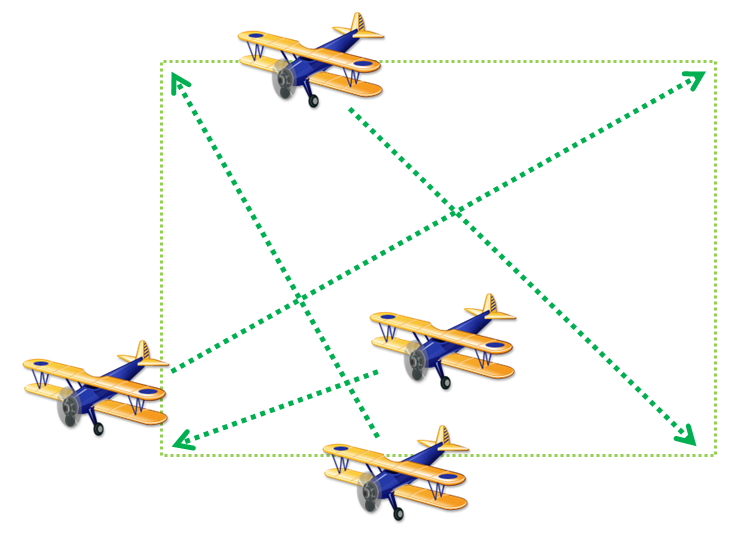
\includegraphics[width=0.49\textwidth]{nearness1.png}}
	%\hspace{7mm}
	\subfigure[Good]{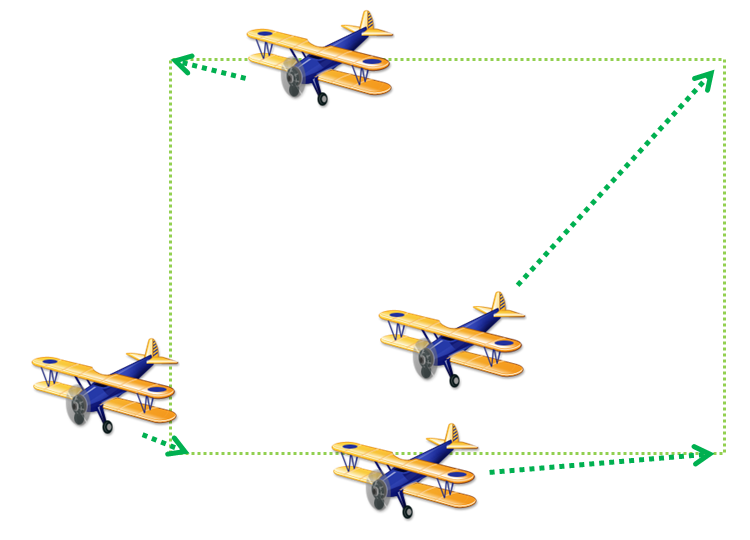
\includegraphics[width=0.49\textwidth]{nearness2.png}}
	\caption{Assignments of aircrafts on the rectangular formation.}	
	\label{nearnessfig}
\end{figure}

\begin{example}
	In Figure \ref{nearnessfig}, 
	the left picture illustrates a bad case in which each aircraft takes the poor path
	compared to the path for the case of the right picture.
	We can guess that this case causes increasing unwanted collisions and 
	more time needed in order to be in the formation.
\end{example}

\begin{definition}[Included-Angle Graph]
	Consider the collection of $ N $ homogeneous agents.
	For $ N $ position vectors $ \psi_i \in \R^m $ for the agents,
	The weighted undirected graph $ \GRP $ with $ N $ vertices is the \textbf{included-angle graph} if
	the graph $ \GRP $ is complete and 
	the each weight $ \theta_{ij} $ of the edge between two vertices $ i $ and $ j $ is 
	the included-angle of two vectors $  \psi_i^c $ and $ \psi_j^c $ as follows.
	\begin{equation}\begin{split}\label{angleweight}
		\psi_i^c &= \psi_i - c, \\
		\psi_j^c &= \psi_j - c, \\
		\theta_{ij} &=  \begin{cases} 
			s \cos^{-1} \left( 
			\frac{	{\psi_i^c}^T \psi_j^c }{\Vert \psi_i^c \Vert \Vert \psi_j^c \Vert} \right)  
			& \text{if } \Vert \psi_i^c \Vert \Vert \psi_j^c \Vert \neq 0, \\ 
			0 & \text{otherwise} \\ \end{cases}	\\
	\end{split}\end{equation}
	where $ c $ is the average of $ \psi_i, i \in [1, N] $ 
	which will be the center of position vectors, and $ s $ is a scalar.
\end{definition}

\begin{definition}[Included-Angle Matrix $ \Theta $]	
	Consider a graph with $ N $ vertices.
	A $ N \times N $ weighted adjacency matrix $ \Theta $ of the included-angle graph is 
	the \textbf{included-angle matrix} if
	\begin{equation}\begin{split}
		\Theta =& \lbrace \theta_{ij} \rbrace \in \R^{N \times N}, \\
		\theta_{ij}=& \text{the weight of the edge} \\
			&\text{between vertices $i$ and $j$ like \eqref{angleweight} }.\\
	\end{split}\end{equation}
\end{definition}

\begin{example}
	For the formation vector $ \zeta $ in Example \ref{exfvector}
	corresponding Figure \ref{trivehicles}, 
	if we select each $ \zeta_i $ as the position vector $ \psi_i $, 
	then the included-angle matrix $ \Theta $ is as follows.
	\begin{equation}
		\Theta = \left[ \begin{array}{ccc } 
		0 & 120 & 120 \\
		120 & 0 & 120 \\
		120 & 120 & 0 \\		
		\end{array} \right]
	\end{equation}
	where $ s=\frac{180}{\pi} $, and $ c=\left[ 0, \frac{-2\sqrt{3}}{3} \right]^T $.
\end{example}

For the equation \eqref{pdynamics},
let a graph $ \GRP_1 $ be the included-angle graph 
for the $ N $ subvectors $ \zeta_i $ like \eqref{fvector} 
of the formation vector $ \zeta $ as position vectors,
and analogously let a graph $ \GRP_2 $ be the included-angle graph 
for the initial outputs of the agents as position vectors.
%Let a graph $ \GRP_1 $ be the included-angle graph 
%for the initial outputs of the agents as position vectors,
%and analogously let a graph $ \GRP_2 $ be the included-angle graph 
%for the $ N $ subvectors $ \zeta_i $, $ 1 \leq \forall i \leq N $ 
%of the formation vector $ \zeta $ in \eqref{fvector} as position vectors.
If we respectively choose $ A_1 $ and $ A_2 $ 
as the included-angle matrices of the graph $ \GRP_1 $ and $ \GRP_2 $,
then, we can get the dynamical system to achieve its solution $ P $ such that $ P_\infty $
approximates the permutation matrix that minimizes $ \Vert PA_1 - A_2 P \Vert_F^2 $
through the equation \eqref{pdynamics}.
Therefore, once the error from an approximation of the permutation matrix is acceptable\footnote
{If $ P_\infty $ is not exactly a permutation matrix, we cannot actually say that 
it is a permutation invariant formation with $ P_\infty $ 
due to the approximation error which makes the assignment on a formation be confused.
But, one can consider the relaxed matrix which is almost a permutation matrix such that
its error can be arbitrarily reduced.},
the steady state solution $ P_\infty $ of the above system can be used for 
the permutation invariant formation tracking problem. Moreover, the matrix $ P_\infty $ minimizes 
the differences of the included angles.
%the included-angles of the agents in the formation tracking.
%the nearness in the sense of the direction of the agent to be in the formation.

% \subsubsection{Response of Assignment Dynamics}
\subsubsection{Formation Vector for Actual Agents}

From Theorem \ref{pdynamicsthm}, because of a dynamical approach, the solution $ P $ 
has the transient response which is not exactly a permutation, 
and even in the steady state response, $ P $ could not be a permutation
since $ P_\infty $ is an approximation of a permutation matrix.
Thus, we should think about how to apply the matrix $ P $ for the formation tracking.
Now, we simply suggest the formation vector $ \zeta_v $, which is designed for virtual agents,
multiplied by $ P $ as the new formation vector $ \zeta $ for actual agents as shown below.

\begin{definition}[Assignment Dynamics]\label{asigndyndef}
	Consider the collection of $ N $ homogeneous agents, 
	of which each has the $ m $-dimensional output.
	Suppose that $ A_1 $ and $ A_2 $ are respectively the $ N \times N $ included-angle matrices
	with respect to a graph $ \GRP_1 $ and $ \GRP_2 $ with $ N $ vertices.
	The graph $ \GRP_1 $ is the included-angle graph 
	for the $ N $ subvectors $ \zeta_{vi}(0) $ like \eqref{fvector} 
	of the formation vector $ \zeta_v(t) $ as position vectors, and
	the graph $ \GRP_2 $ is the included-angle graph 
	for the initial outputs of the agents as position vectors.
	The following dynamical system is the \textbf{assignment dynamics} 
	which maps the formation vector $ \zeta_v(t) $ for virtual agents 
	to the formation vector $ \zeta(t) $ for actual ones.
	\begin{equation}\begin{split}\label{assigndynamics}
		\dot{P} &= P \left( P^T A_2 P A_1 - A_1 P^T A_2 P \right)
					-k P \left( (P \circ P)^T P -P^T (P \circ P) \right) \\
		\zeta(t) &= \left( P \otimes I_m \right) \zeta_v(t) \\
	\end{split}\end{equation}
	where $ P(0) = I_N $ and $ k $ is a positive constant.
	Furthermore, we say that the matrix $ P $ minimizes  
	\textbf{the nearness in the sense of the included-angle matching} 
	of the agents in the group.	
\end{definition}


\begin{remark}	
	The nearness in the sense of the included-angle matching is distinguished
	from the physical closeness for an agent to get a position in the formation.
	In Figure \ref{homomatchfig}, 
	Graphs $ \GRP_1 $, $ \GRP_2 $, $ \GRP_3 $ and $ \GRP_4 $ are identical.
	For a weighted graph matching problem, these four graphs are the same class 
	so that each graph trivially has the identical matrix as permutation matrix to the others. 
	But, the formation vectors corresponding the graphs might be different 
	from each other because a formation vector is not invariant under the rotation. 
	Consequently, for a permutation invariant tracking problem,	we can say that 
	the permutation matrix $ P $ from the assignment dynamics \eqref{assigndynamics}
	sequentially assigns the virtual agents in the group 
	to the actual agents through one case of its class 
	of which all formation vectors have the same included-angle matrices.
	In other words, we have the permutation matrix $ P $ as one of the matrices in the same class,
	and we don't know which one will be selected in the class by the assignment dynamics.
\end{remark}

\begin{figure}[htp]
	\centering
	\subfigure[Graph $ \GRP_1 $]{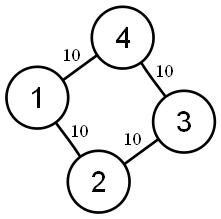
\includegraphics[width=0.24\textwidth]{homogenity1.png}}
	\subfigure[Graph $ \GRP_2 $]{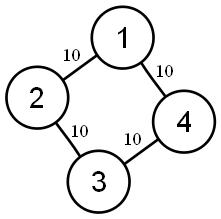
\includegraphics[width=0.24\textwidth]{homogenity2.png}}
	\subfigure[Graph $ \GRP_3 $]{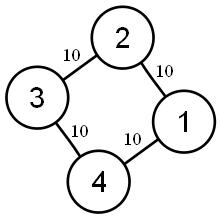
\includegraphics[width=0.24\textwidth]{homogenity3.png}}
	\subfigure[Graph $ \GRP_4 $]{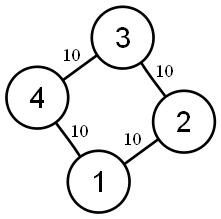
\includegraphics[width=0.24\textwidth]{homogenity4.png}}
	\caption{Identical graphs for a weighted graph matching problem.}	
	\label{homomatchfig}
\end{figure}


\begin{remark}[Transient Response of Assignment Dynamics]
	For the system \eqref{assigndynamics}, 
	a Lyapunov function is given in \cite{graphmatch} as follows.
	\begin{equation}
		V(P) = \frac{1}{2} \Vert PA_1 -A_2P \Vert_F^2 
			+k \frac{2}{3} tr \left( P^T \left( P -\left( P \circ P \right) \right)\right)
	\end{equation}
	In such cases, $ \dot{V(P)} $ is non-increasing which means that $ P $
	will converge to a local minimum that will be $ P_\infty $.
	In other words, $ P $ is continuously changing forward to minimize the cost such as \eqref{matchcost}.
	Therefore, the transient response of the system is still valuable 
	to assign virtual agents on the formation besides the steady state response. 
	This transient assignment will be shown as the morphing of the formation
	while the matrix $ P $ comes into effect as the weight for changing shape.
\end{remark}


\subsection{Integrated Tracking Control}

\begin{theorem}\label{intgthm}
	Consider the collection of the agent systems \eqref{formationsys}. 	
	Assume that $ f_i $, $ g_i $ and $ h_i $ are respectively identical 
	for $ 1 \leq \forall i \leq N $	that means homogeneous systems,
	and	the Laplacian matrix $ L $ stands for an output sensing graph $ \GRP $ of the agents
	in which each agent $ i $ can sense the outputs of its neighbors $ \NBR_i $.
	For a formation vector $ \zeta_v $,
	if \begin{itemize}
		\item 	the agent is globally state feedback input-output linearizable,
		\item	each output of agents is absolutely measurable by itself, 		
		\item	the tracking dynamics of the agent is bounded input bounded state stable,
		\item	the directed graph $ \GRP $ of the Laplacian $ L $ is 
				strongly connected or has a single leader component,
		\item	and $ s^{\rho_j} + \lambda_i k_{j\rho_j} s^{\rho_j-1} + \cdots + \lambda_i k_{j1} $ 
				are Hurwitz polynomials for $ \forall \lambda_i \in \lambda(L) $, 				
				such that $ \lambda_i \neq 0 $, $ 1 \leq \forall j \leq m $,
	\end{itemize}
	then, the permutation invariant formation tracking problem is approximately solvable 
	with the additional assignment dynamics. 
	And, the controller $ u_i $ would be as shown below.
	\begin{equation}\begin{split}\label{integratethm}
		\dot{P} &= P \left( P^T A_2 P A_1 - A_1 P^T A_2 P \right)
					-k P \left( (P \circ P)^T P -P^T (P \circ P) \right) \\
		\zeta &= \left( P \otimes I_m \right) \zeta_v \\
		u_i &= -\A^{-1}(x_i) \left( L_f^\rho h(x_i)			
		    - \left( \frac{1}{\vert \NBR_i \vert} \sum_{l \in M}
				K_{l}  \sum_{j \in \NBR_i } (y_i - y_j -  \zeta_{i} + \zeta_{j}) ^{(l-1)}  
				+  \zeta_{i}^{(\rho)}(t) \right)\right)\\			
	\end{split}\end{equation} 	
	where the matrix $ A_1 $ and $ A_2 $ are defined as Definition \ref{asigndyndef},
	$ P(0) = I_N $, $ k $ is a positive constant. And,
	$ \rho $, $ M $, $ L_f^\rho h(\cdot) $ , $ K_l $, $ \A $ 
	and $ \zeta_{i}^{(\rho)} $ are like \eqref{trackingthmwhere}.
	Moreover, each agent goes through the nearest path in the sense of
	the included-angle matching of the agents. 
\end{theorem}

\begin{proof}
	By Theorem \ref{formationcontrolthm}, the collection of multiple agents would be in the formation
	which is represented by the formation vector $ \zeta $. And,
	$ \lim_{t \to \infty} P = P_\infty $ approximates the permutation matrix
	which maps the formation vector $ \zeta_v $ to $ \zeta $.
	From Theorem \ref{pdynamicsthm}, we can arbitrarily reduce the approximation error by choosing larger $ k $.
	Consequently, we can resolve the permutation invariant formation problem remaining 
	a permutation error which appears as a distortion of the formation in the steady states
	while minimizing the nearness in the sense of the included-angle matching by Definition \ref{asigndyndef}.
\end{proof}

\begin{remark}
	The controller $ u_i $ in \eqref{integratethm} is a decentralized one that means 
	it is sufficient that each agent $ i $ only knows the information about its neighborhoods $ \NBR_i $.
	For a permutation invariant formation tracking, however, 
	every agents should be aware of the global knowledge. For instance, 
	each agent builds $ A_1 $ and $ A_2 $ matrices to be assigned to the virtual agent at initial time.	
	But, these kinds of global information are disposable after setup of an assignment dynamics. 
	It is undesired that every agents keep the maintenance of the global knowledge.
	Therefore, the decentralized control is also valid for a permutation invariant formation tracking problem
	as well as a formation tracking problem.
\end{remark}
	
Until now, we have studied about a formation. The word of the formation appears in a variety of fields.
Generally, the formation indicates the shape of a group to collaborate a common mission.
In this chapter, we mathematically defined what the formation is,
and we introduced the formation tracking problem. 
To resolve this problem, we quantified the formation by the formation matrix and vector.
And the output tracking by relative references presented in the previous chapter 
was applied to this problem.
We also discussed the permutation of agents. 
If the agents in the group are homogeneous, each agent can be replaced by others.
For taking the advantage of the homogeneity, a weighted graph matching problem was employed
and a dynamical approach was introduced as its solver.
Finally, we described the nearness with the included-angle concept,
and integrated the formation tracking problem and the weighted graph matching problem into
the permutation invariant formation tracking problem.



\chapter{Example}

\section{Multiple Homogeneous Nonholonomic Mobile Robots}

\subsection{Modeling a Mobile Robot}

Consider the following simple kinematic model of a mobile robot described 
in Figure \ref{fig:kinematic_model}
that shows a vehicle with two tires subject to the constraint
of the wheels which is allowed to roll and spin, but not to slip. 

\begin{figure}[htp]
	\centering
	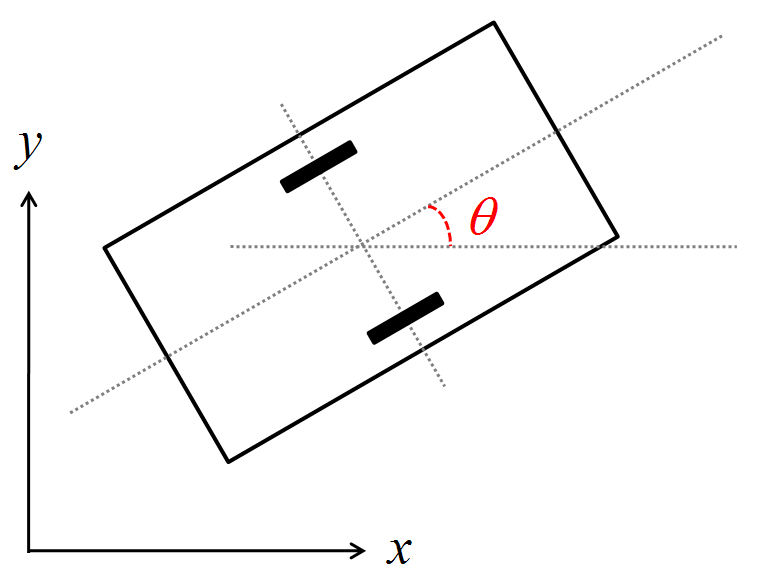
\includegraphics[width=0.50\textwidth]{kinematic_model.png}
	\caption{Kinematic model of a mobile robot.}
	\label{fig:kinematic_model}
\end{figure}

The constraint restricts the wheels 
such that the velocity of their sideways is to be zero as shown below.
\begin{equation}\begin{split}\label{eq:model}
	\dot{x} \sin \theta-\dot{y} \cos \theta &=0
\end{split}\end{equation}
where $ x $ and $ y $ are the configuration of the robot by the $ xy $ location of the wheels,
$ \theta $ is the angle of the body with respect to the horizontal.

The equation \eqref{eq:model} is a kind of \textbf{Pfaffian constraint} 
that is composed of velocity conditions expressed by $ A(q)\dot{q}=0 $ 
where $ q \in $ configuration space $ \mathbb{Q} $, $ A(q)\in \R ^{k \times n} $ 
represents a set of $ k $ velocity constraints. 
It is said to be \textbf{integrable} if there exists a vector-valued
function $ h:\mathbb{Q} \to \R^{k} $ such that 
$ A(q)\dot{q}=0 $ $ \Longleftrightarrow $ $ \frac{\partial h}{\partial q}\dot{q}=0 $. 
This $ h $ can be represented locally as \textbf{algebraic constraints} 
on the configuration space like $ h_{i}(q)=0 $, $ i \in \left[ 1,k \right]  $ 
that is said to be \textbf{holonomic constraint}; 
the motion of system is restricted to \textbf{a smooth hypersurface} 
in the (unconstrained) $\mathbb{Q}$.
Otherwise, it is \textbf{not integrable} if there is no $ h $ satisfying the above condition. 
In such cases, the constraint is \textbf{nonholonomy}; 
the instantaneous velocities of the system are constrained to an $ n-k $ dimensional subspace, 
but the set of reachable configuration is not restricted to some $ n-k $ dimensional hypersurface\footnote
{For more detailed explanation, see \cite{bi:murray, sastry}.}.
		
From a Pfaffian constraints \eqref{eq:model}, we can make it possible that 
converting the constraints to the state space equation \eqref{eq:ss}
through taking an adequate variable substitution.
Generally, the conversion for a control system is to select null vectors $ v_{i} $ 
from the null space of $ A(q) $ such that $ A(q)\dot{q}=0 $,
with which we have the differential equation 
like $ \dot{q}=v_{1} u_{1} + \ldots + v_{k} u_{k} $. 

For the constraints \eqref{eq:model} of the mobile robot,
suppose that $ u_{1} $ and $ u_{2} $ is input variables for a control system. 
If we respectively choose $ u_1 $ and $ u_2 $ as the driving velocity and the steering velocity,
then, one can have the dynamical system as shown below.
\begin{equation}\begin{split}\label{eq:ss}
	\dot{x}&=u_1 \cos \theta\\
	\dot{y}&=u_1 \sin \theta\\
	\dot{\theta}&=u_2\\	
\end{split}\end{equation} 
where $ u_{1} $ is the velocity of the wheels, 
and $ u_{2} $ is the velocity of the angle of the wheels.

\subsection{Input-output feedback linearization}

For state feedback input-output linearization, 
we cannot directly get the well defined the vector relative degree of the system \eqref{eq:ss}.
In order to achieve the relative degree, we employ a dynamic extension \cite{isidori} 
while introducing the acceleration of the wheels $ u_3 $ as new input variable 
as follows.
\begin{equation}\begin{split}\label{eq:ss2}
	\dot{x}&=u_1 \cos \theta\\
	\dot{y}&=u_1 \sin \theta\\
	\dot{\theta}&=u_2\\	
	\dot{u_1}&=u_3\\	
\end{split}\end{equation} 

Consider the dynamical system \eqref{eq:ss2}.
We investigate the vector relative degree.
Let
\begin{equation}\begin{split}\label{deffgh}
	f(\x) &= \left[ \begin{array}{c } u_1 \cos \theta \\
		u_1 \sin \theta \\
		0 \\ 0 \\	\end{array} \right], \quad 
	g(\x) = \left[ \begin{array}{cc } \vert & \vert \\
		g_1(\x) & g_2(\x) \\
		\vert & \vert \\ \end{array} \right]
		= \left[ \begin{array}{cc } 0 & 0 \\		0 & 0 \\		1 & 0 \\
		0 & 1 \\	\end{array} \right],\\
	h(\x) &= \left[ h_1(\x),h_2(\x) \right]^T = \left[ x,y \right]^T \\
\end{split}\end{equation}
where $ \x = \left[ x,y, \theta, u_1 \right]^T $ and $ \U = \left[ u_2,u_3 \right]^T $.

\begin{remark}
	The system \eqref{eq:ss2} is rewritten as the simple form as shown below.
	\begin{equation}\begin{split}
		\dot{\x} &= f(\x) + g(\x) \U \\
		\y &= h(\x) \\
	\end{split}\end{equation}
\end{remark}

Now, we have the global vector relative degree 
$ \rho=\left[ \rho_1, \rho_2  \right]^T=\left[2,2  \right]^T $ if $ u_1 \neq 0 $.
Because,
\begin{equation}\begin{split}
	& L_{g_j} h_k (\x) = 0, \qquad 1 \leq \forall j,k \leq 2,\\
	%& L_{g_1} h_1 (\x) = \left[ 1, 0, 0, 0 \right] \left[ 0, 0, 1, 0 \right]^T =0, \\
	%& L_{g_1} h_2 (\x) = \left[ 0, 1, 0, 0 \right] \left[ 0, 0, 1, 0 \right]^T =0, \\
	%& L_{g_2} h_1 (\x) = \left[ 1, 0, 0, 0 \right] \left[ 0, 0, 0, 1 \right]^T =0, \\
	%& L_{g_2} h_2 (\x) = \left[ 0, 1, 0, 0 \right] \left[ 0, 0, 0, 1 \right]^T =0, \\	
	& \A (\x)=\left[ \begin{array}{cc } 
		L_{g_1} L_f h_1 (\x) & L_{g_2} L_f h_1 (\x) \\
		L_{g_1} L_f h_2 (\x) & L_{g_2} L_f h_2 (\x) \\
	\end{array} \right] 
	=\left[ \begin{array}{cc } -u_1 \sin \theta & \cos \theta \\
		u_1 \cos \theta & \sin \theta \\ 
		\end{array} \right] \\	
\end{split}\end{equation}
where $ \A (\cdot) $ is nonsingular except $ u_1 = 0 $. 
When $ u_1 = 0 $ with the proposed controller discussed in earlier chapters, 
the mobile robot is only stuck at the position where the robot is in the formation. 
Thus, we don't need to worry about this singularity via no control input at that position.

The system \eqref{eq:ss2} is globally state feedback input-output linearizable without zero dynamics
since the sum of $ \rho_1 $, $ \rho_2 $ is the dimension of $ \x $. 
Therefore, we can keep away the boundedness of the tracking dynamics
for the condition of Theorem \ref{formationcontrolthm} and \ref{intgthm}.

\subsection{Multiple Homogeneous Mobile Robots}
At this moment, we consider $ N=6 $ agents of multiple homogeneous mobile robots
of which each agent has the identical dynamical system as shown below, and 
the output of the agent is absolutely measurable by itself\footnote
{It is nothing but the guarantee of state feedback input-output linearization for the agent
without help from the others}.
\begin{equation}\begin{split}
	\dot{\x_i} &= f(\x_i) + g(\x_i) \U_i \\
	\y_i &= h(\x_i) \\
\end{split}\end{equation}
for all $ i \in \left[ 1,6 \right] $ where $ \x_i =\left[ x_i, y_i, \theta_i, u_{i1} \right]^T $,
$ \U_i = \left[ u_{i2}, u_{i3} \right]^T $
and the vector fields $ f,g,h $ are like \eqref{deffgh}.

\subsection{Formation Configuration}
\begin{figure}[htp]
	\centering
	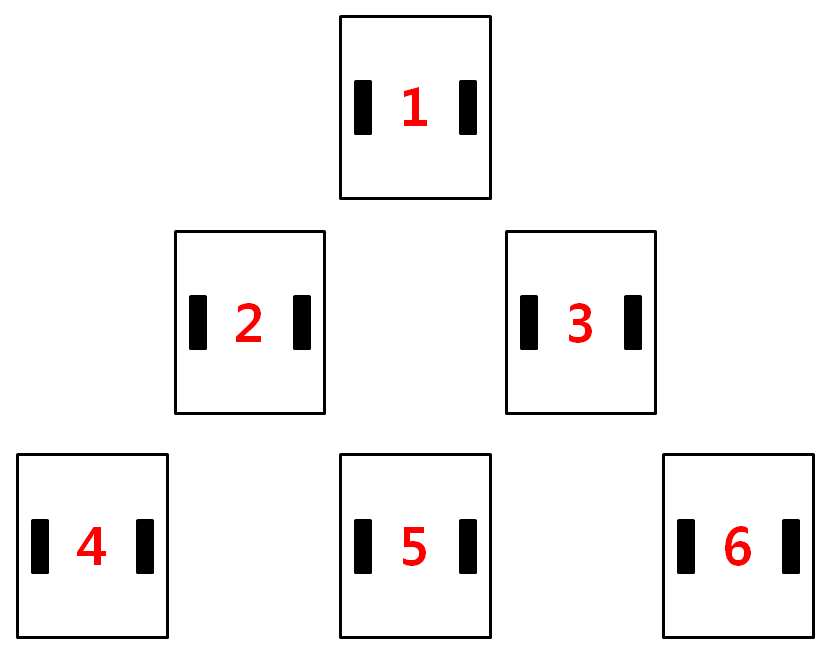
\includegraphics[width=0.40\textwidth]{formation.png}
	\caption{Triangular formation of $ 6 $ multiple homogeneous agents. 
			The number on body is the index of the agent.}
\end{figure}

\subsubsection{Formation Matrix and Vector}
\begin{equation}\begin{split}\label{fmatrixandvector}
	F(t)&=\begin{tiny}
		50\left[ \begin {array}{cccccc} 0&2+\sin \left( t \right) &-2-\sin \left( t \right) &
		4+2\sin \left( t \right) &0&-4-2\sin \left( t \right) \\0&4+2\sin \left( t \right) &
		4+2\sin \left( t \right) &8+4\sin \left( t \right) &8+4\sin \left( t \right) &
		8+4\sin \left( t \right) \\-2-\sin \left( t \right) &0&-4-2\sin \left( t \right) &
		2+\sin \left( t \right) &-2-\sin \left( t \right) &-6-3\sin \left( t \right) \\
		-4-2\sin \left( t \right) &0&0&4+2\sin \left( t \right) &4+2\sin \left( t \right) &
		4+2\sin \left( t \right) \\2+\sin \left( t \right) &4+2\sin \left( t \right) &
		0&6+3\sin \left( t \right) &2+\sin \left( t \right) &-2-\sin \left( t \right) \\
		-4-2\sin \left( t \right) &0&0&4+2\sin \left( t \right) &4+2\sin \left( t \right) &
		4+2\sin \left( t \right) \\-4-2\sin \left( t \right) &-2-\sin \left( t \right) &
		-6-3\sin \left( t \right) &0&-4-2\sin \left( t \right) &-8-4\sin \left( t \right) \\
		-8-4\sin \left( t \right) &-4-2\sin \left( t \right) &-4-2\sin \left( t \right) &0&0&0\\
		0&2+\sin \left( t \right) &-2-\sin \left( t \right) &4+2\sin \left( t \right) &0&
		-4-2\sin \left( t \right) \\-8-4\sin \left( t \right) &-4-2\sin \left( t \right) &
		-4-2\sin \left( t \right) &0&0&0\\4+2\sin \left( t \right) &6+3\sin \left( t \right) &
		2+\sin \left( t \right) &8+4\sin \left( t \right) &4+2\sin \left( t \right) &0\\
		-8-4\sin \left( t \right) &-4-2\sin \left( t \right) &
		-4-2\sin \left( t \right) &0&0&0\end {array} \right] 
		\end{tiny}
		,
	\\
	\zeta(t)&= \left[ \begin{array}{c } \zeta_1(t) \\ \zeta_2(t) \\ 
				\zeta_3(t) \\\zeta_4(t)\\\zeta_5(t)	\\ \zeta_6(t) \end{array} \right]
		% = \begin{footnotesize}
		% \left[ \begin {array}{c} 0\\0\\
		% -100-50\,\sin \left( t \right) \\-200-100\,\sin \left( t \right) \\
		% 100+50\,\sin \left( t \right) \\-200-100\,\sin \left( t \right) \\
		% -200-100\,\sin \left( t \right) \\-400-200\,\sin \left( t \right) \\
		% 0\\-400-200\,\sin \left( t \right) \\
		% 200+100\,\sin \left( t \right) \\-400-200\,\sin \left( t \right) \end {array} \right] 
		% \end{footnotesize}
		,\qquad \begin{array}{l } 
			\zeta_1(t)=\left[ 0, 0 \right]^T,\\
			\zeta_2(t)=\left[ -100-50\,\sin \left( t \right), -200-100\,\sin \left( t \right) \right]^T,\\
			\zeta_3(t)=\left[ 100+50\,\sin \left( t \right), -200-100\,\sin \left( t \right) \right]^T,\\
			\zeta_4(t)=\left[ -200-100\,\sin \left( t \right), -400-200\,\sin \left( t \right) \right]^T,\\
			\zeta_5(t)=\left[ 0, -400-200\,\sin \left( t \right) \right]^T,\\
			\zeta_6(t)=\left[ 200+100\,\sin \left( t \right), -400-200\,\sin \left( t \right)\right]^T\\
		\end{array}
\end{split}\end{equation}

Our goal is that the collection of the $ 6 $ agents will be in the formation described by \eqref{fmatrixandvector}.
As shown above, the formation is varying with respect to time and the shape of which is triangular.

\subsection{Connectivity of Agents}

\begin{figure}[htp]
	\centering
	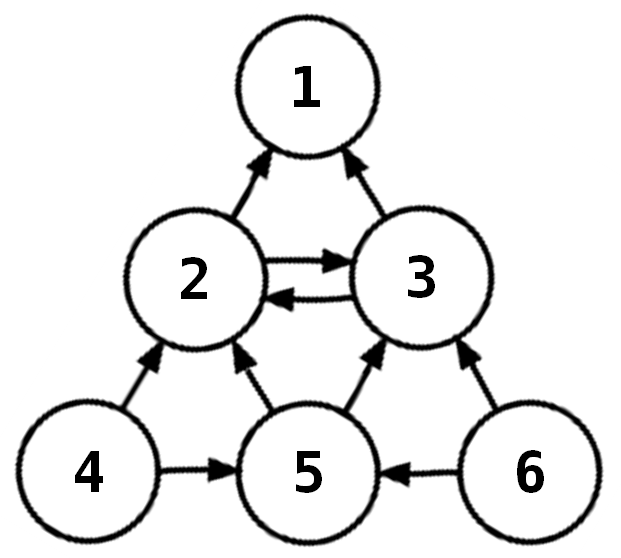
\includegraphics[width=0.40\textwidth]{laplacian.png}
	\caption{Output sensing graph of the agents for Laplacian matrix \eqref{exlaplacian}.
	This graph represents that the agent $ i $ can sense the outputs of its neighbors $ \NBR_i $.
	The agent $ 1 $ is the single leader of the group by the connectivity of the graph.}
	\label{connect}
\end{figure}

Figure \ref{connect} describes the connectivity of the mobile robot group.
Each agent $ i $ can only sense the outputs of its neighbor $ \NBR_i $ defined in \eqref{sensingnbr}.
Thus, the individual agent has not to know all outputs of the agents 
which induces the formation controller to be decentralized.
And Figure \ref{connect} shows that there is one leader component which is determined
by the connectivity of the graph corresponding its Laplacian matrix \eqref{exlaplacian}
as we already discussed in Section \ref{graphtheory}.

\begin{equation}\begin{split}\label{sensingnbr}
	\NBR_1 &= \lbrace \rbrace, \quad\quad\;\,
	\NBR_2 = \lbrace1, 3 \rbrace, \quad \NBR_3 = \lbrace 1, 2\rbrace,\\
	\NBR_4 &= \lbrace 2, 5\rbrace, \quad	
	\NBR_5 = \lbrace 2, 3\rbrace, \quad	\NBR_6 = \lbrace 3, 5\rbrace
\end{split}\end{equation}

% laplacian matrix
\begin{equation}\label{exlaplacian}
	L=\left[ \begin{array}{cccccc } 
	0 & 0 & 0 & 0 & 0 & 0 \\
	-\frac{1}{2} & 1 & -\frac{1}{2} & 0 & 0 & 0 \\
	-\frac{1}{2} & -\frac{1}{2} & 1 & 0 & 0 & 0 \\
	0 & -\frac{1}{2} & 0 & 1 & -\frac{1}{2} & 0 \\
	0 & -\frac{1}{2} & -\frac{1}{2} & 0 & 1 & 0 \\
	0 & 0 & -\frac{1}{2} & 0 & -\frac{1}{2} & 1 \\		
	\end{array} \right],\qquad
	\lambda(L)=\lbrace0, 0.5, 1, 1.5  \rbrace
\end{equation}

\subsection{Decentralized Formation Controller}
Now, we examine the gain of the controller.
If we choose
\begin{equation} 
	k_{11} = 300,\quad k_{12} = 50 ,\quad	k_{21} = 300,\quad k_{22} = 50,
\end{equation}
then the following equations are guaranteed to be Hurwitz polynomials.
\begin{equation}
	s^{\rho_j} + \lambda_i k_{j\rho_j} s^{\rho_j-1} + \cdots + \lambda_i k_{j1} 
\end{equation}
where $ \forall \lambda_i \in \lambda(L) $ 
such that $ \lambda_i \neq 0 $ and $ 1 \leq \forall j \leq m=2 $.
Therefore, by Theorem \ref{formationcontrolthm},
we finally achieve the decentralized formation controller $ \U_i $ as shown below.
\begin{equation}\begin{split}\label{excontroller}
	\U_i &= -\A^{-1}(\x_i) \left( L_f^\rho h(\x_i)			
		- \left( \frac{1}{\vert \NBR_i \vert} \sum_{l \in M}
			K_{l}  \sum_{j \in \NBR_i } (\y_i - \y_j -  \zeta_{i} + \zeta_{j}) ^{(l-1)}  
			+  \zeta_{i}^{(\rho)}(t) \right)\right)\\			
\end{split}\end{equation} 	
where
\begin{equation}\begin{split}
	\A^{-1}(\x_i) &=\left[ \begin{array}{cc } -\frac{1}{u_{i1}} \sin\theta_i &  \frac{1}{u_{i1}} \cos\theta_i \\ 
					\cos\theta_i & \sin\theta_i \\ \end{array} \right], \\
	L_f^\rho h(\x_i) &= \left[ \begin{array}{c } 0 \\ 0 \\ \end{array} \right], \qquad	\qquad	
	\zeta_i^{(\rho)} (t) % = \zeta_i^{(2)}(t) 
		= \left[ \begin{array}{c } \zeta_{i1}^{(2)}(t) \\ \zeta_{i2}^{(2)}(t) \\ \end{array} \right],\\	
	K_1 &= \left[ \begin{array}{cc } 300 & 0 \\ 0 & 300 \\ \end{array} \right], \qquad
	K_2 = \left[ \begin{array}{cc } 50 & 0 \\ 0 & 50 \\ \end{array} \right], \\
	M &=\lbrace 1, 2\rbrace. \\
\end{split}\end{equation}

\subsection{Permutation Invariant Formation}
In this subsection, 
we consider the permutation invariant formation control 
talked about in Section \ref{permutationinvariantformation}.
For the formation \eqref{fmatrixandvector}, 
if the initial states of the agents are given like \eqref{initstates},
we have the included angle matrices $ A_1 $ and $ A_2 $ as follows.
% included angle matrix 
\begin{equation}\begin{split}
	A_1&=\begin{footnotesize} \left[ \begin{array}{cccccc } 
         0&   56.3099&   56.3099&  123.6901&  180.0000&  123.6901\\
   56.3099&         0&  112.6199&   67.3801&  123.6901&  180.0000\\
   56.3099&  112.6199&         0&  180.0000&  123.6901&   67.3801\\
  123.6901&   67.3801&  180.0000&         0&   56.3099&  112.6199\\
  180.0000&  123.6901&  123.6901&   56.3099&         0&   56.3099\\
  123.6901&  180.0000&   67.3801&  112.6199&   56.3099&         0\\  
	\end{array} \right]\end{footnotesize}, \\
	A_2&=\begin{footnotesize}\left[ \begin{array}{cccccc } 
         0&   42.1485&  153.9344&  147.1317&   31.1422&  179.0182\\
   42.1485&         0&  163.9171&  104.9832&   73.2907&  138.8333\\
  153.9344&  163.9171&         0&   58.9338&  122.7923&   25.0838\\
  147.1317&  104.9832&   58.9338&    0.0000&  178.2739&   33.8501\\
   31.1422&   73.2907&  122.7923&  178.2739&    0.0000&  147.8760\\
  179.0182&  138.8333&   25.0838&   33.8501&  147.8760&    0.0000\\
	\end{array} \right]\end{footnotesize}
\end{split}\end{equation}
where $ s=\frac{180}{\pi}$ and the initial states of the mobile robots are like
\begin{equation}\begin{alignat*}{3}\label{initstates}
	\x_{1}(0)&=\left[ 0, 0, \frac{90}{180} \pi, 150 \right]^T, 
	&\x_{2}(0)&=\left[ -150, -900, \frac{-70}{180} \pi, 70 \right]^T, \\
	\x_{3}(0)&=\left[ 250, -1600, \frac{-60}{180} \pi, 100 \right]^T, 
	&\x_{4}(0)&=\left[ -300, -1500, \frac{30}{180} \pi, 70 \right]^T, \\
	\x_{5}(0)&=\left[ 150, -800, \frac{90}{180} \pi, 20 \right]^T, 
	&\x_{6}(0)&=\left[ -5, -1550, \frac{-120}{180} \pi, 80 \right]^T 
\end{alignat*}\end{equation}

Consequently, we can resolve the permutation invariant tracking control problem by Theorem \ref{intgthm}
with the additional assignment dynamics as shown below 
while $ \zeta_v $ is substituted with $ \zeta $ of \eqref{fmatrixandvector}
and the new $ \zeta $ of \eqref{exassignmentdynamics} is used as 
the new formation vector of the controller \eqref{excontroller}.
\begin{equation}\begin{split}\label{exassignmentdynamics}
	\dot{P} &= P \left( P^T A_2 P A_1 - A_1 P^T A_2 P \right)
				-k P \left( (P \circ P)^T P -P^T (P \circ P) \right) \\
	\zeta &= \left( P \otimes I_m \right) \zeta_v \\
\end{split}\end{equation}
where $ P(0)=I_6 $ and $ k=1000 $.

\subsection{Simulation Results}
All results in this subsection were simulated with the initial values of \eqref{initstates} on MATLAB.

\subsubsection{Decentralized Formation Tracking Control}

\begin{figure}[htp]
	\centering
	\subfigure[$ x $ trajectories ]{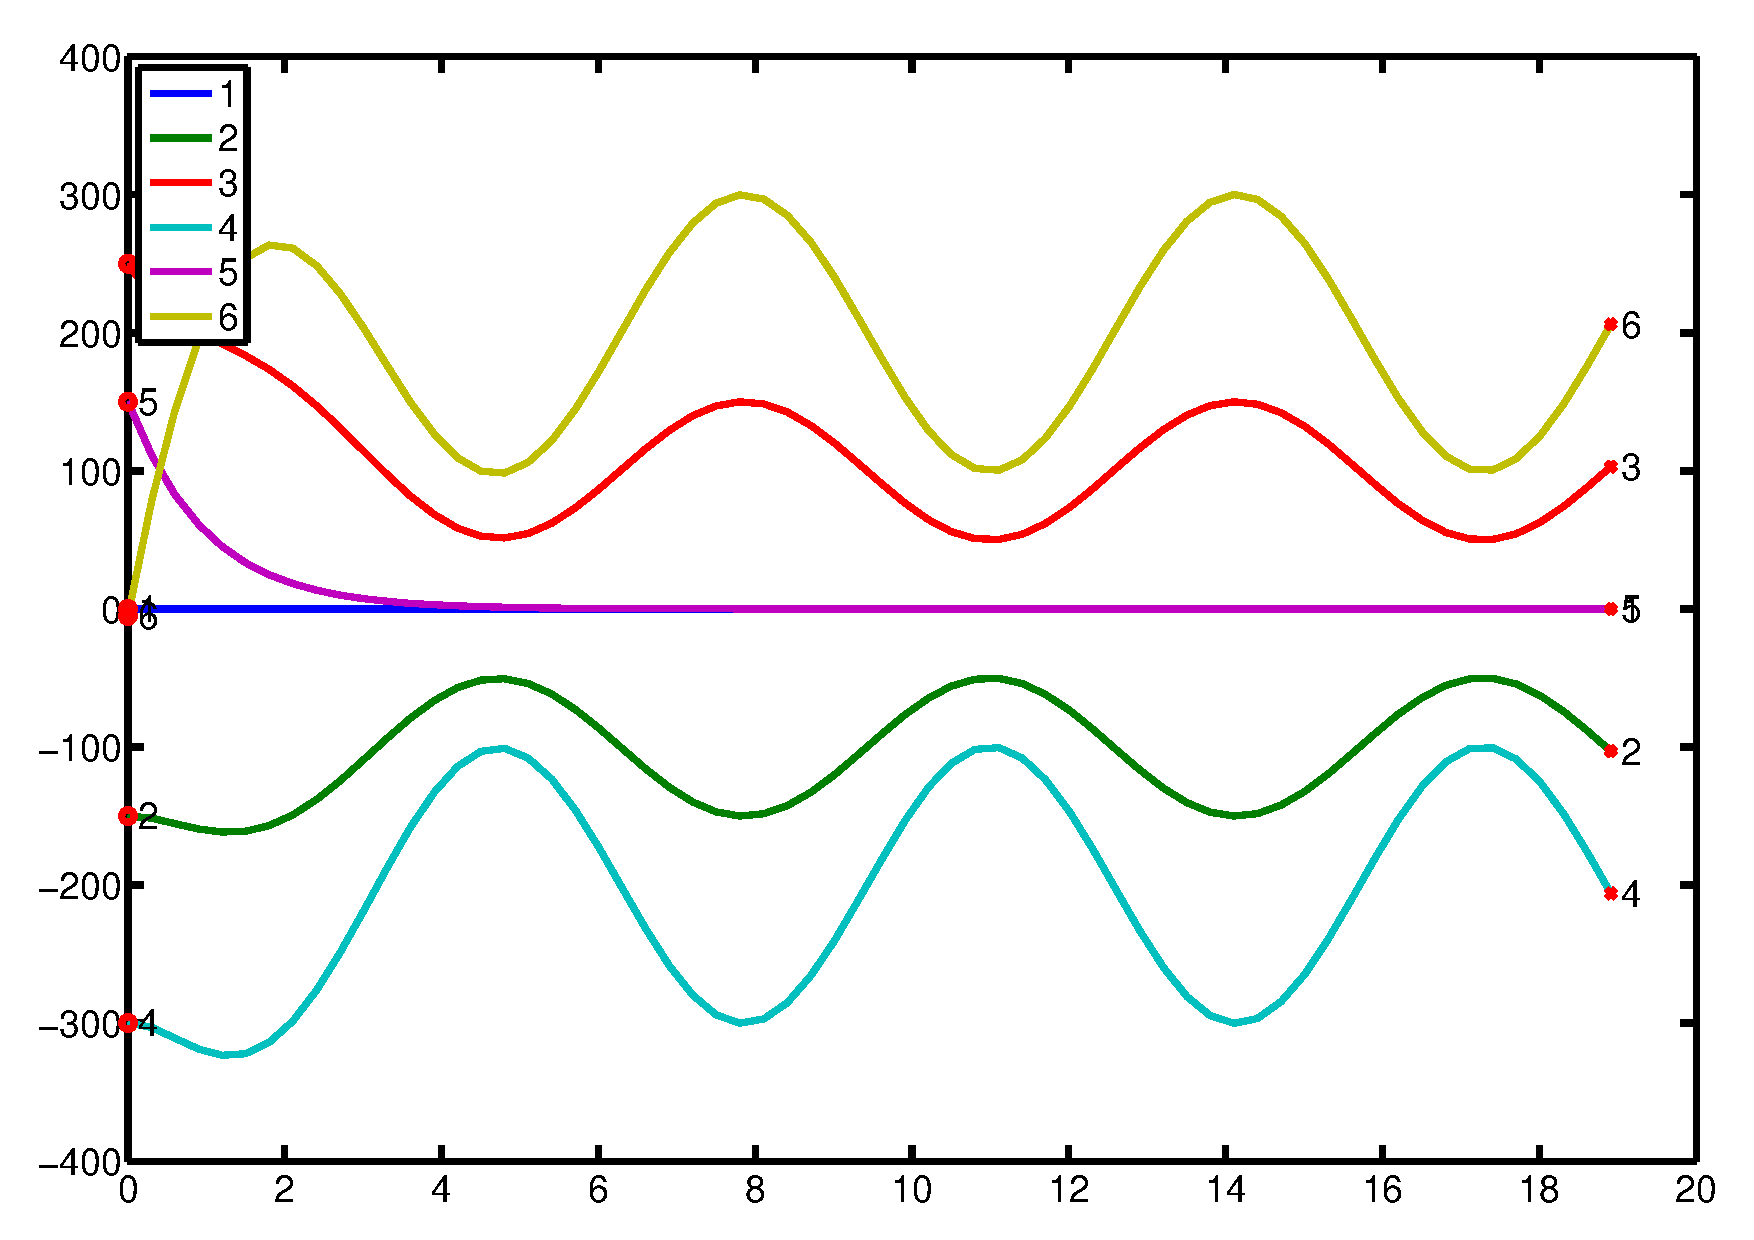
\includegraphics[width=0.49\textwidth]{formationTracking_x.pdf}}
	\subfigure[$ y $ trajectories ]{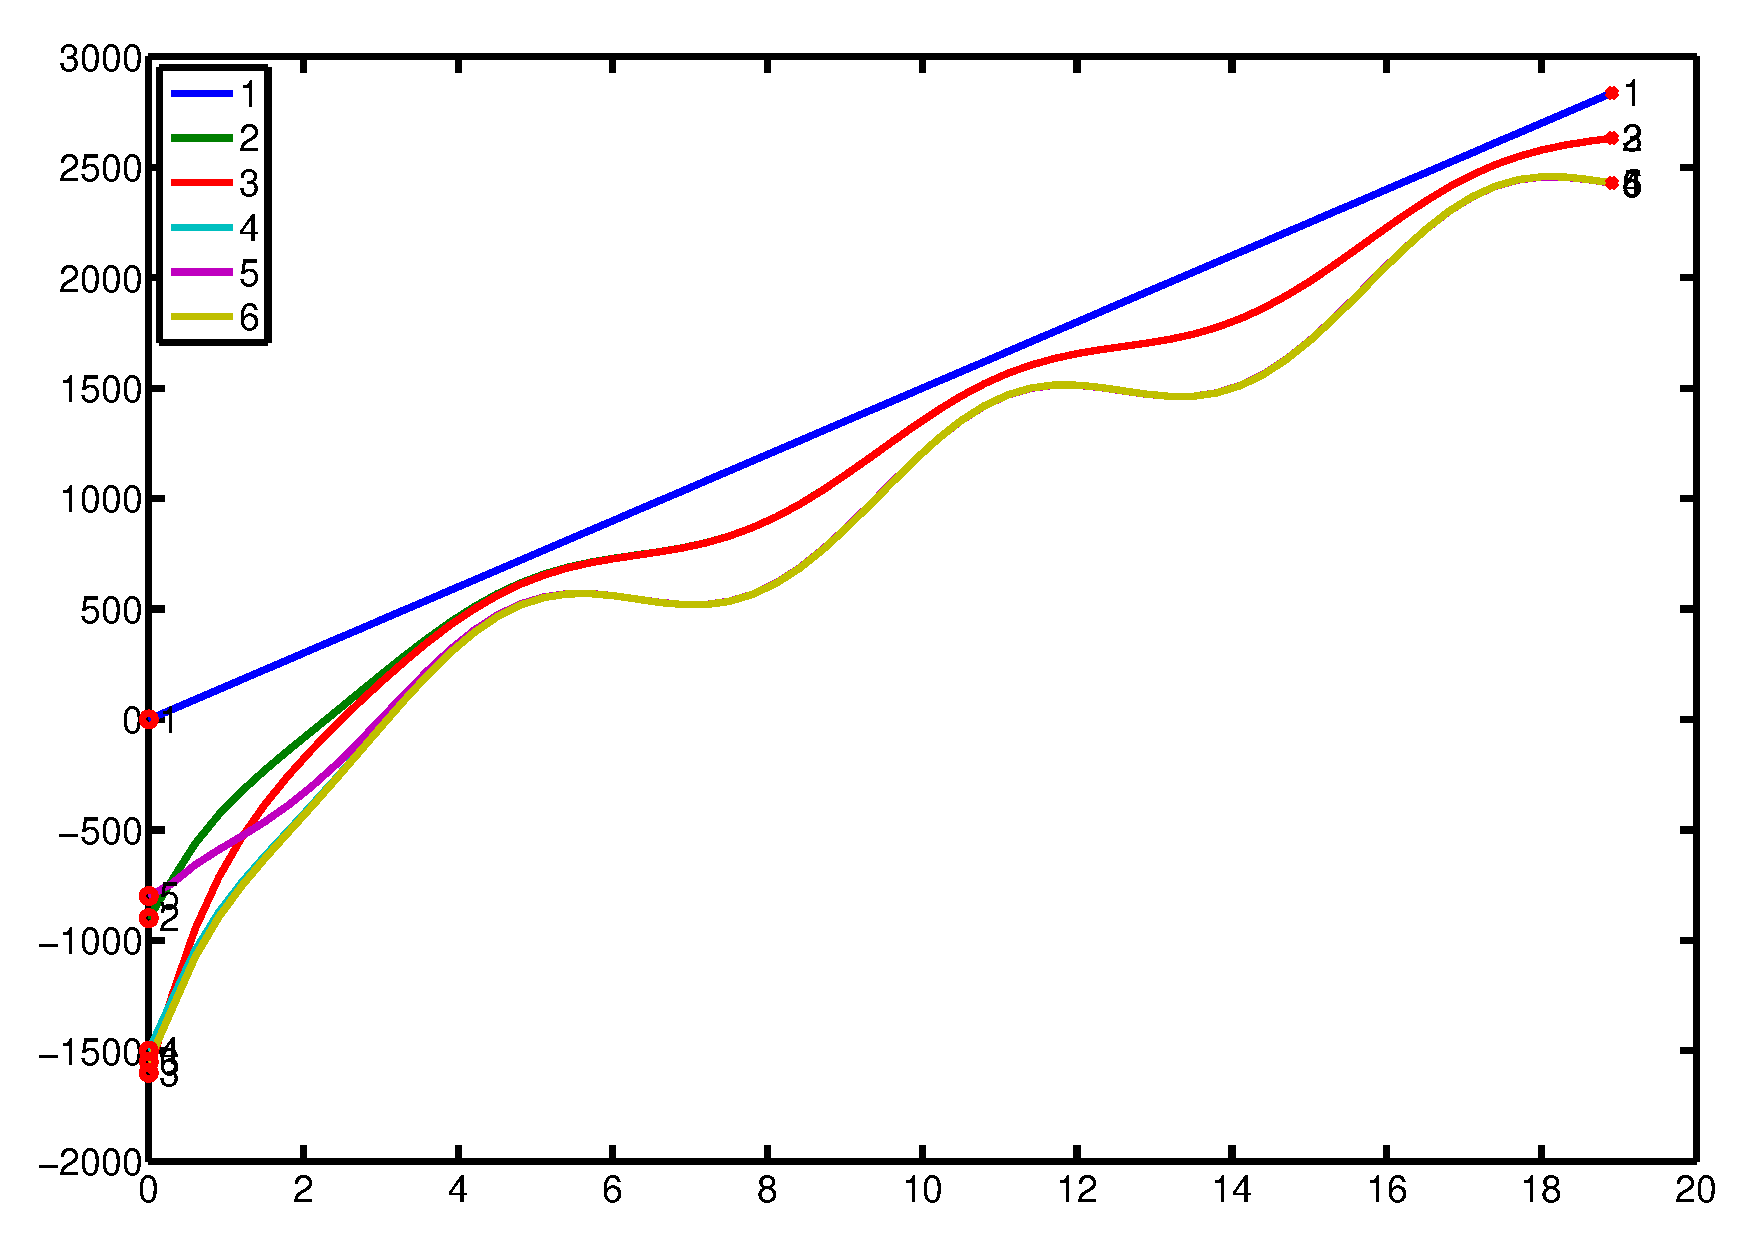
\includegraphics[width=0.49\textwidth]{formationTracking_y.pdf}}	
	\caption{$ x $, $ y $ trajectories of the agents.
		`o' indicates the initial positions of the agents and 
		`x' does the final positions. The number of each line is the index of the agent.}	
\end{figure}

\begin{figure}[htp]
	\centering
	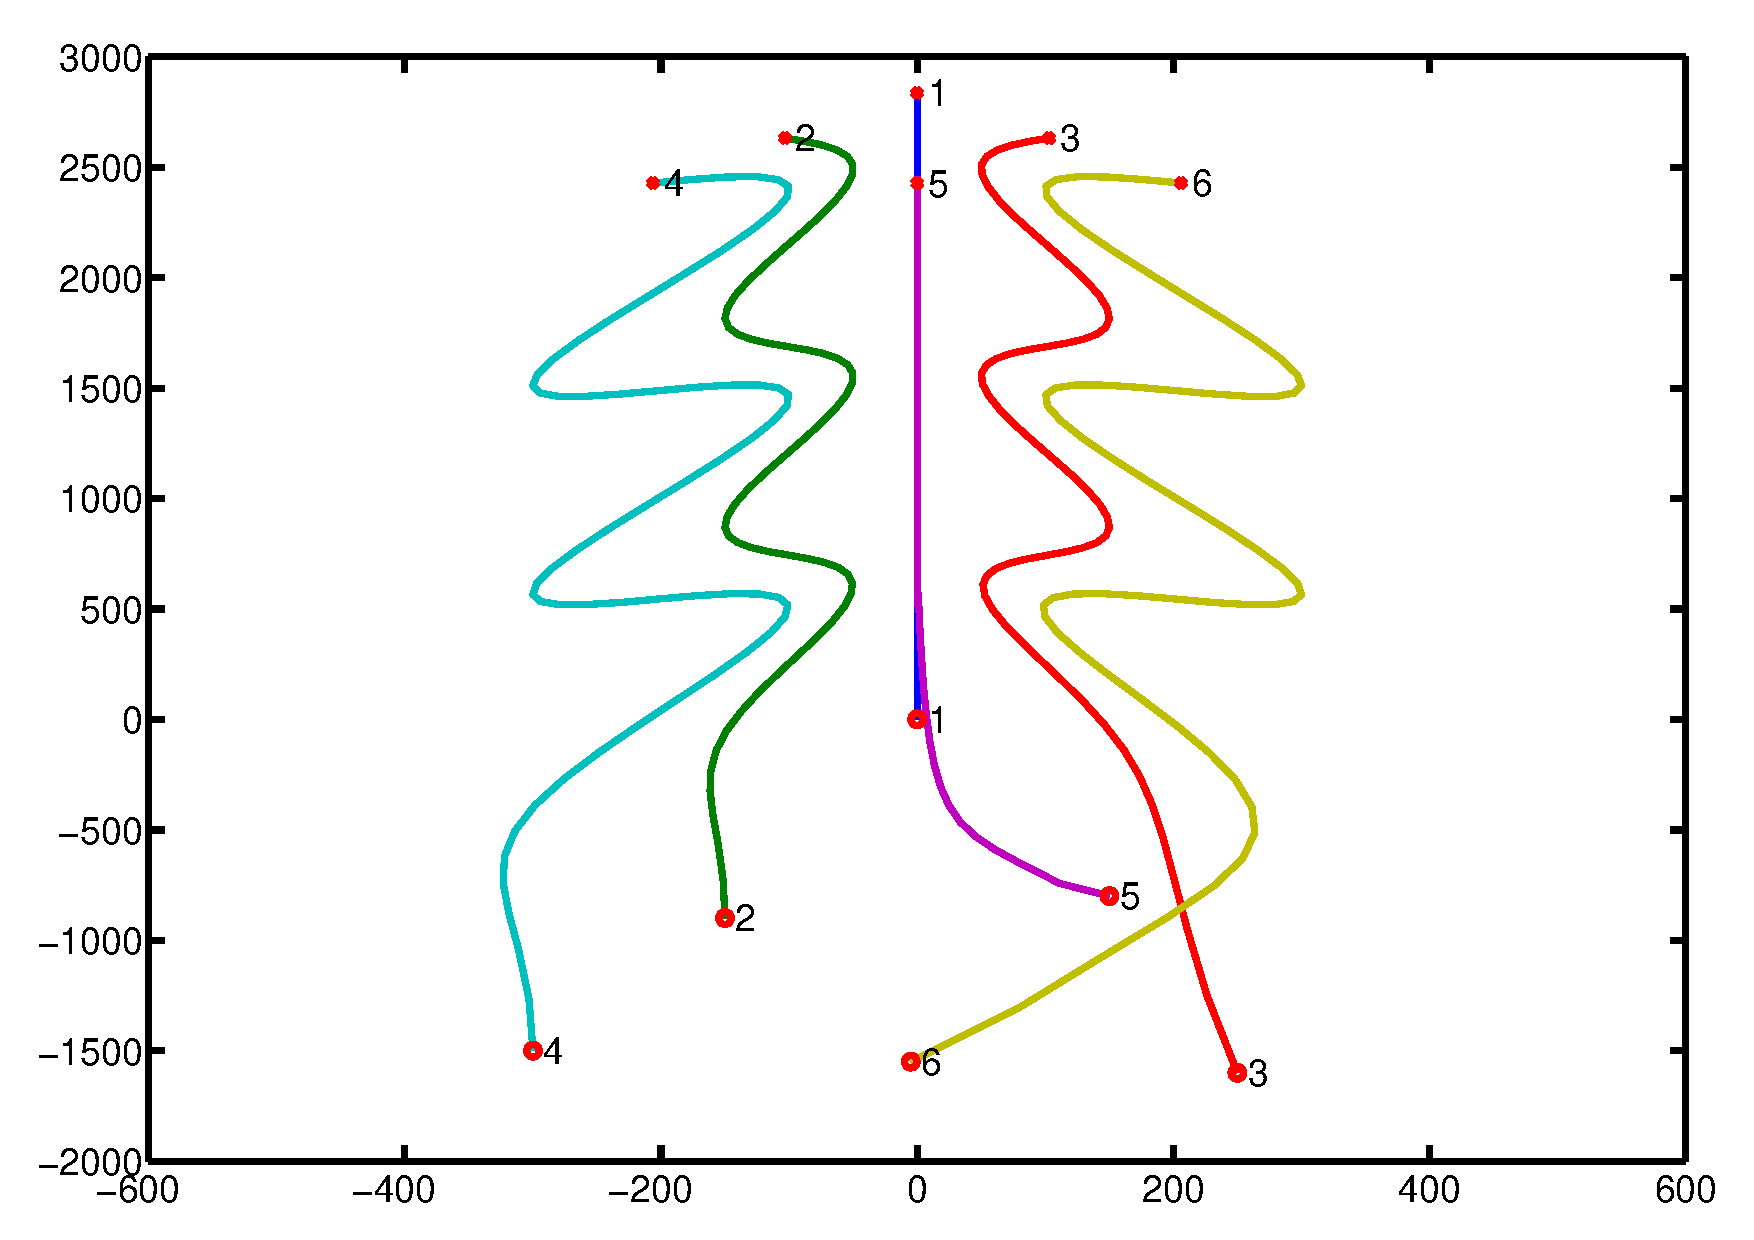
\includegraphics[width=0.99\textwidth]{formationTracking.pdf}
	\caption{Decentralized formation tracking control for \eqref{excontroller}.
		`o' indicates the initial positions of the agents and 
		`x' does the final positions. The number of each line is the index of the agent.}		
\end{figure}

\subsubsection{Permutation Invariant Formation Tracking Control}
The output of assignment dynamics \eqref{exassignmentdynamics} at time $ 50 $ was as shown below.
\begin{equation}
	P(50)=\left[\begin{array}{cccccc}
    1.0019&   -0.0259&   -0.0495&    0.0434&    0.0008&    0.0816\\
    0.0284&    1.0048&   -0.0207&    0.0199&   -0.0273&   -0.0245\\
   -0.0678&    0.0153&   -0.0299&    0.0181&    0.0455&    1.0020\\
   -0.0353&   -0.0114&    0.0173&    0.9776&    0.0460&   -0.0264\\
    0.0504&    0.0265&    1.0030&   -0.0048&   -0.0616&    0.0264\\
    0.0081&    0.0235&    0.0720&   -0.0360&    1.0219&   -0.0386\\
	\end{array}\right]
\end{equation}
which approximated the following matrix $ P_\infty $.
\begin{equation}
	P_\infty=\left[\begin{array}{cccccc}
    1&    0&    0&    0&    0&    0\\
    0&    1&    0&    0&    0&    0\\
    0&    0&    0&    0&    0&    1\\
    0&    0&    0&    1&    0&    0\\
    0&    0&    1&    0&    0&    0\\
    0&    0&    0&    0&    1&    0\\
	\end{array}\right]
\end{equation}


\begin{figure}[htp]
	\centering
	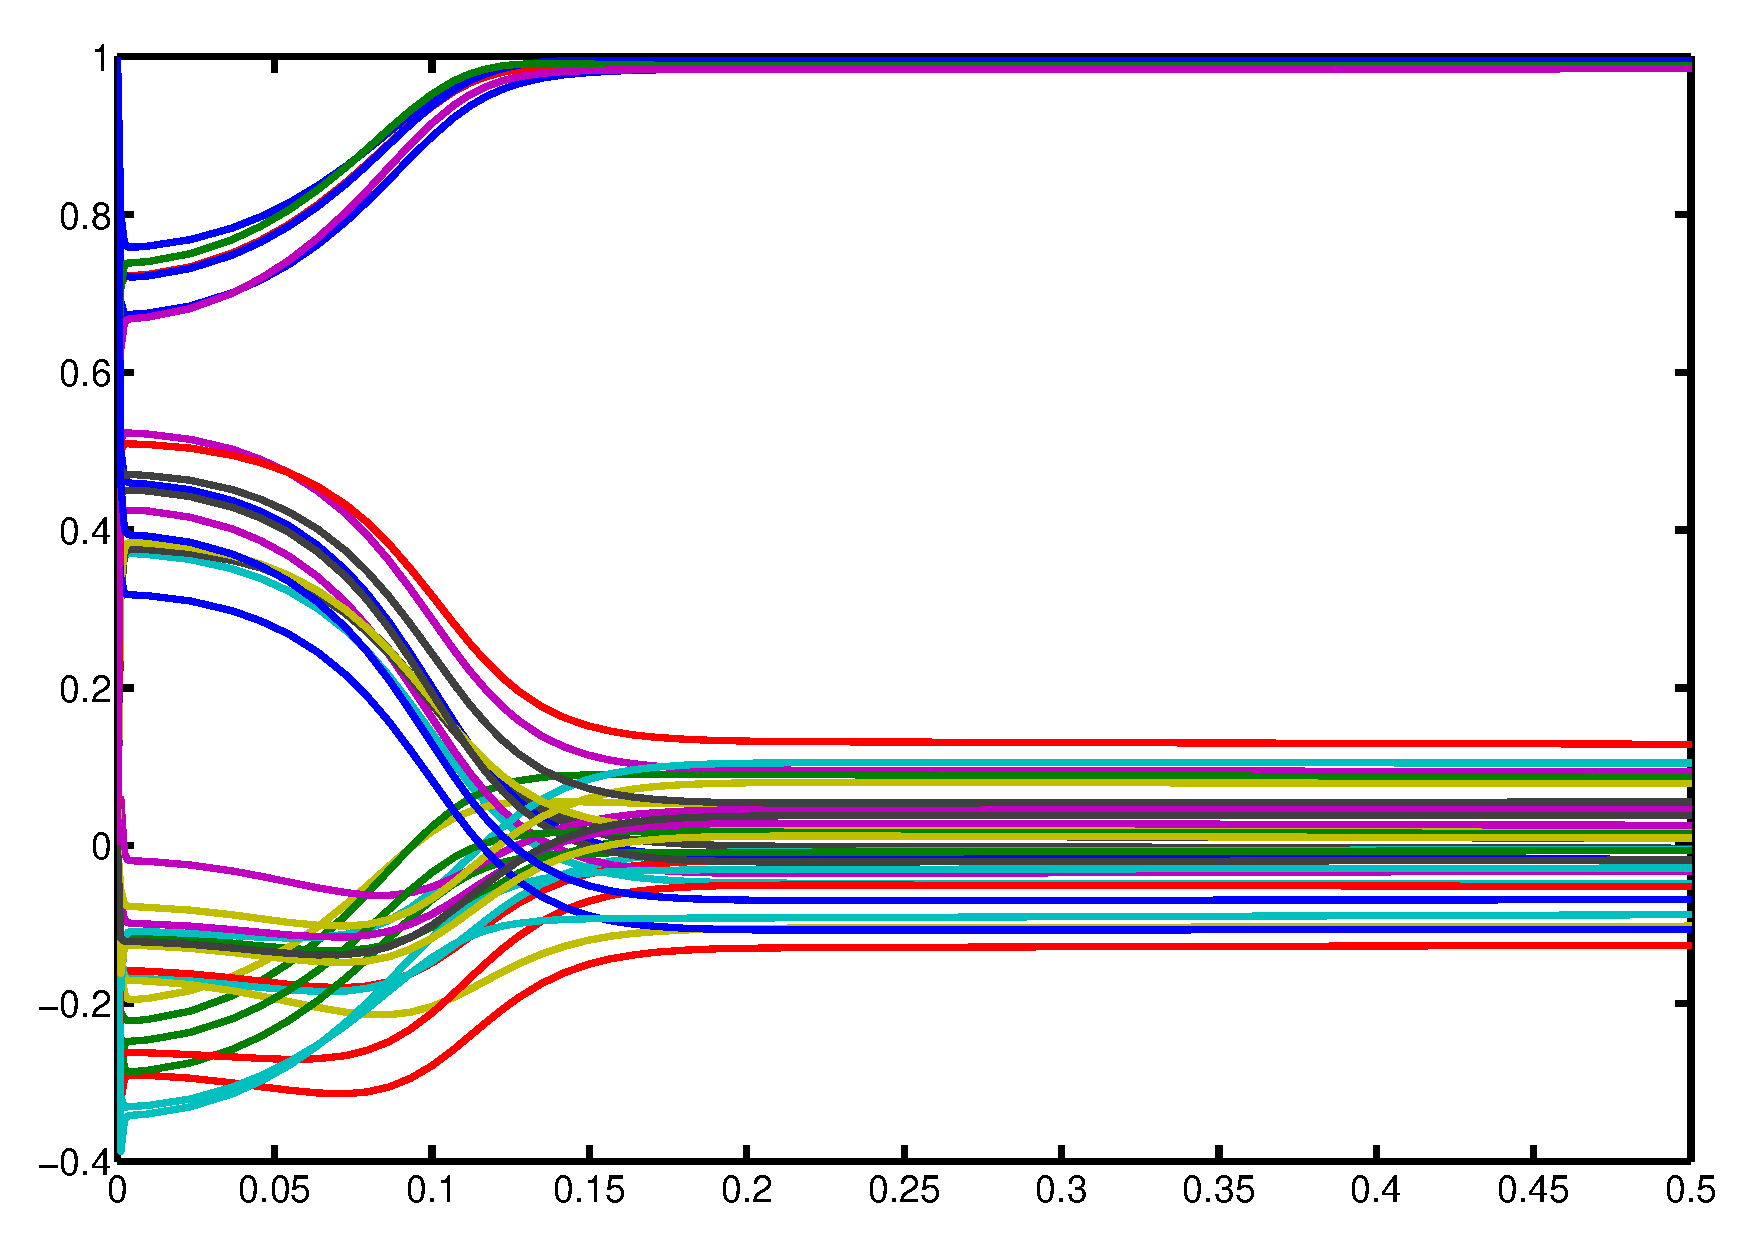
\includegraphics[width=0.60\textwidth]{pdynamics.pdf}
	\caption{Evaluation of the elements of the output matrix $ P $ 
		for the assignment dynamics \eqref{exassignmentdynamics} during $ 0.5 $ time.}	
\end{figure}

\begin{figure}[htp]
	\centering
	\subfigure[$ x $ trajectories]{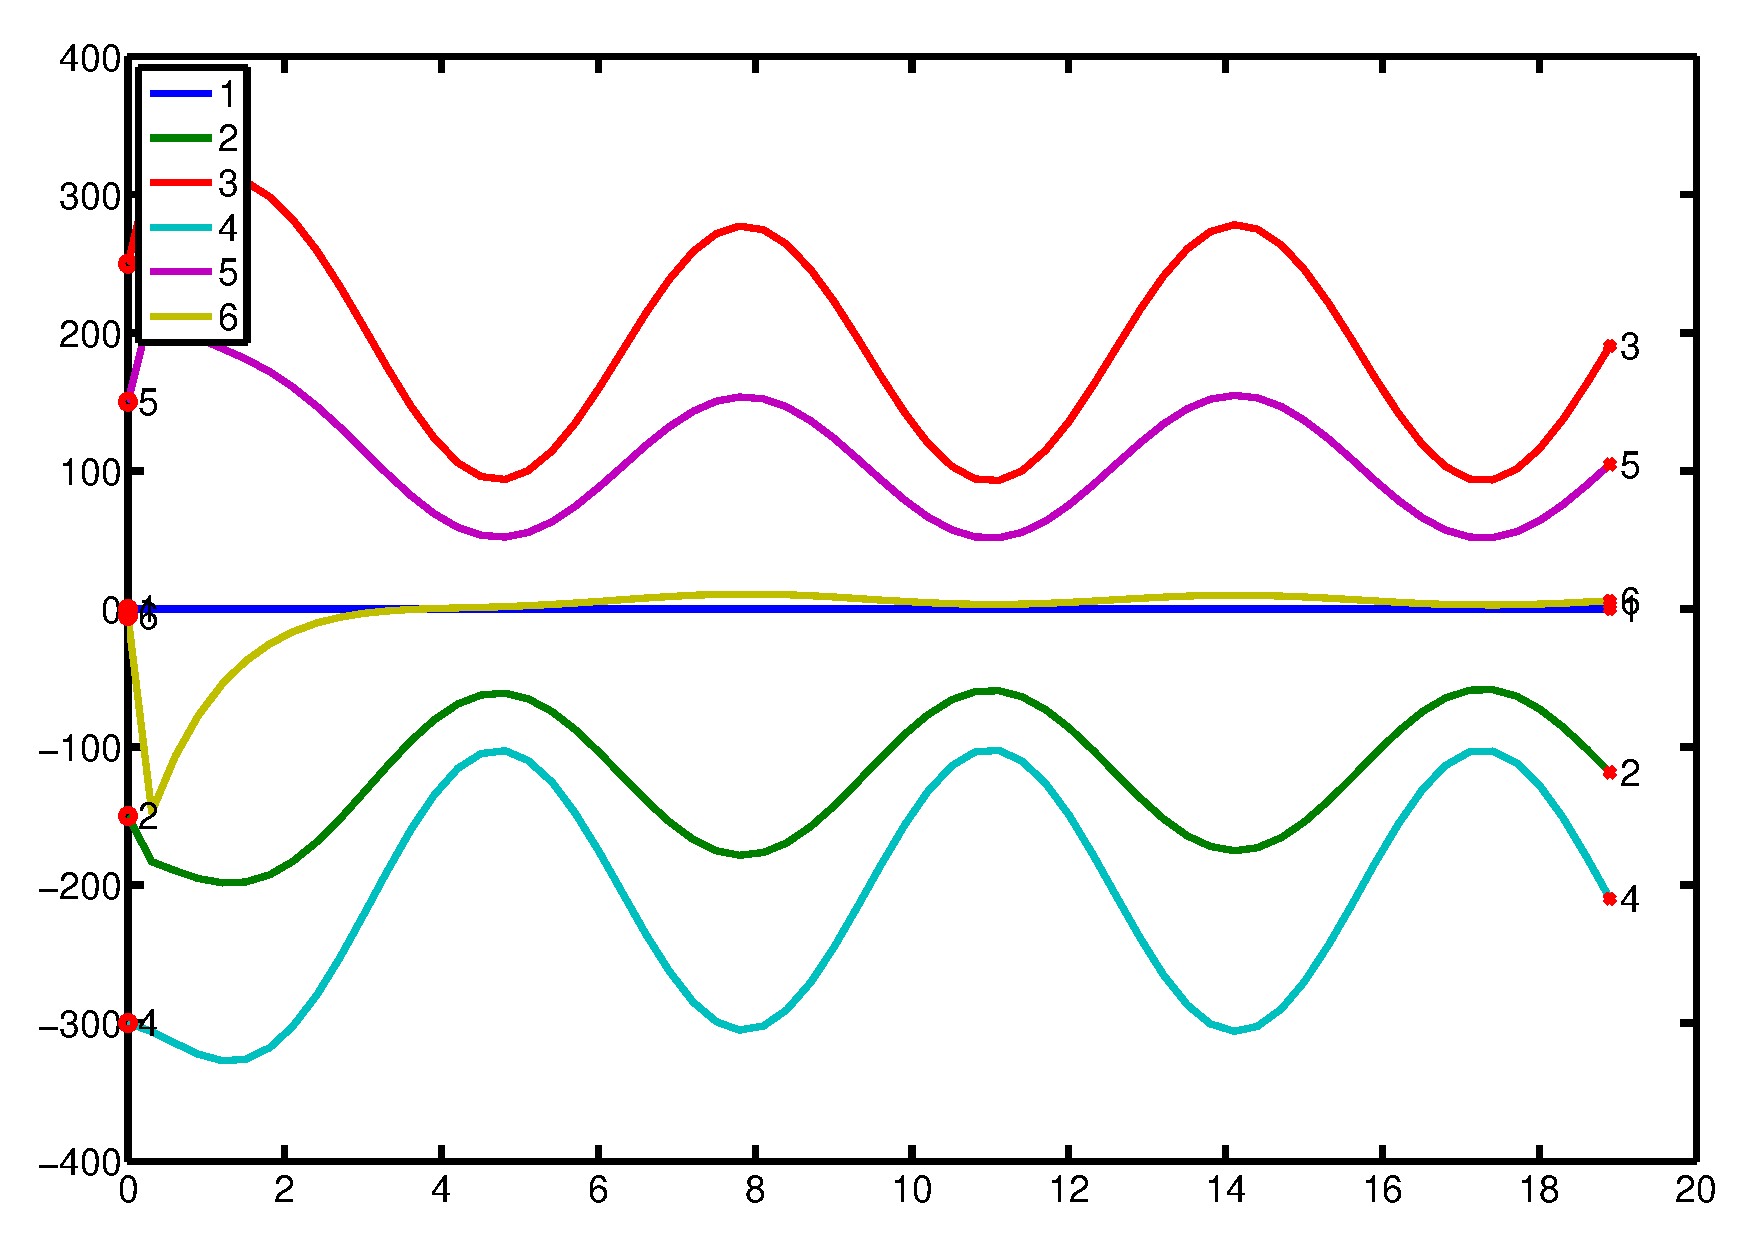
\includegraphics[width=0.49\textwidth]{formationTracking2_x.pdf}}
	\subfigure[$ y $ trajectories]{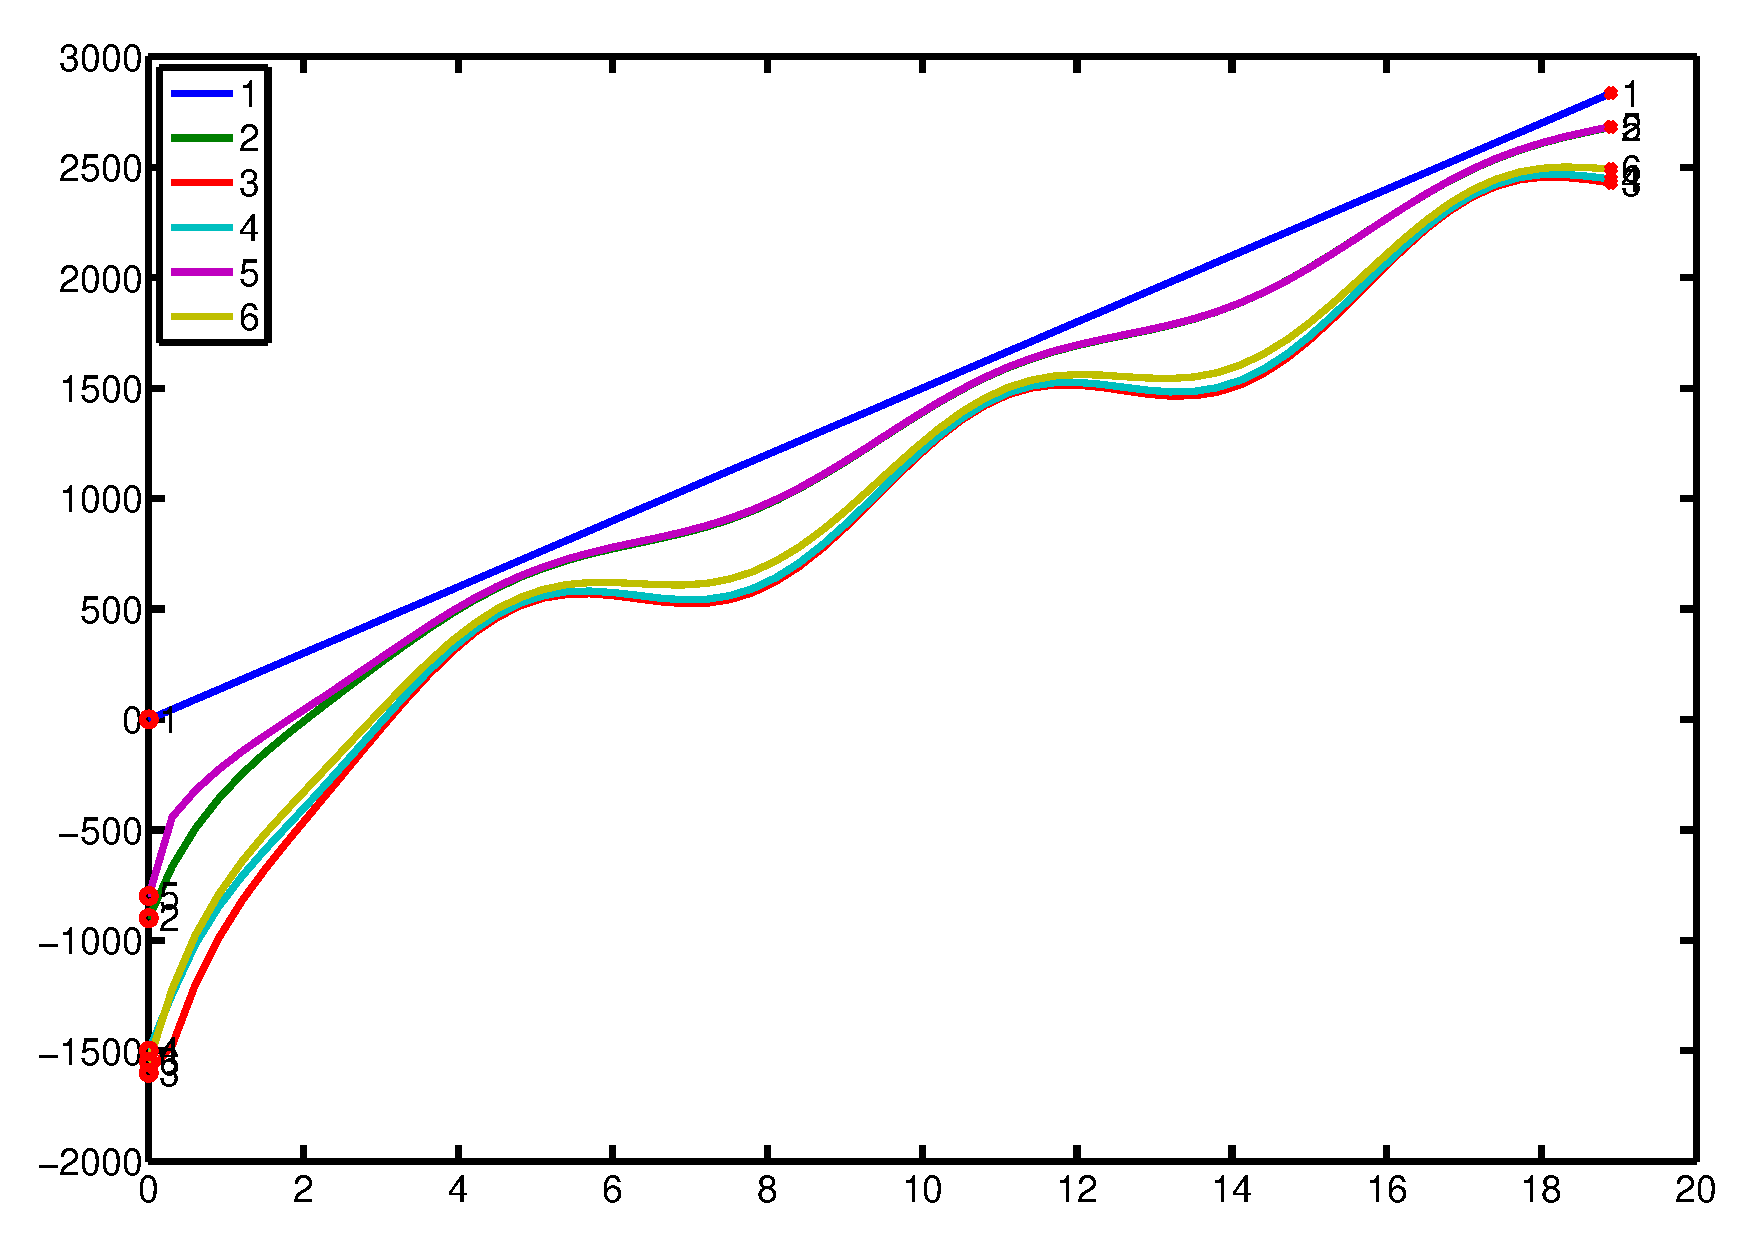
\includegraphics[width=0.49\textwidth]{formationTracking2_y.pdf}}	
	\caption{$ x $, $ y $ trajectories of the agents.
		`o' indicates the initial positions of the agents and 
		`x' does the final positions. The number of each line is the index of the agent.}	
\end{figure}

\begin{figure}[htp]
	\centering
	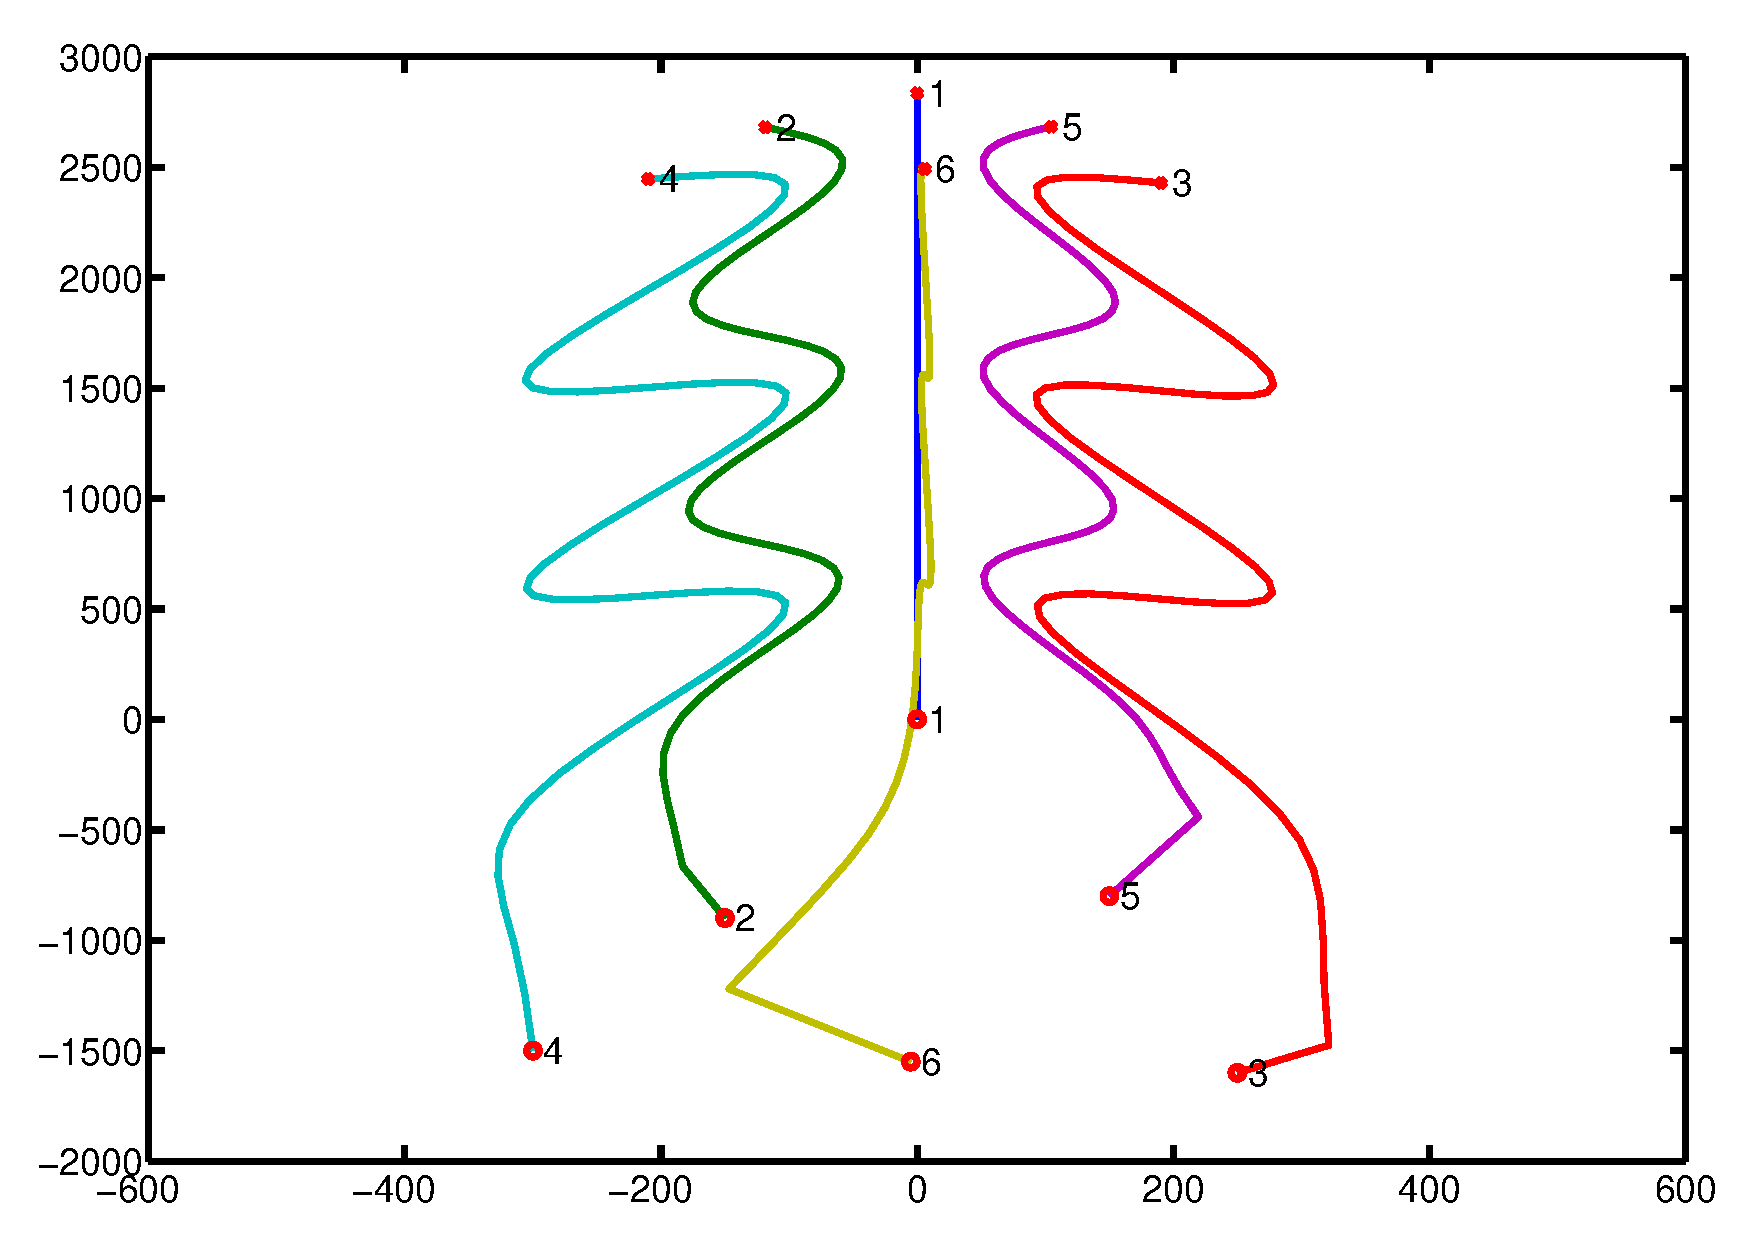
\includegraphics[width=0.99\textwidth]{formationTracking2.pdf}
	\caption{Permutation invariant formation tracking control.
		`o' indicates the initial positions of the agents and 
		`x' does the final positions. The number of each line is the index of the agent.}		
\end{figure}


\chapter{Conclusion}
In this thesis, 
we have considered the decentralized formation tracking control of multiple homogeneous agents.
By the proposed control scheme, the collection of the agents keeps the formation
while the flock of agents can freely move anywhere.

We first discussed the output tracking problem and extended it for multiple homogeneous systems.
The output tracking problem of multiple agents by relative references is that
the differences of the outputs among the agents keep tracking given references.
In order to resolve it, we introduced graph theory.
The properties of the eigenvalue and the null space of Laplacian adjacency matrix 
play a key role to explain the stability of tracking control.
Thus, we analyzed the condition of stability with those properties and developed the tracking controller 
where Laplacian matrix corresponding the connectivity of the agents is strongly connected or
has a single leader component.

Formation generally are described as a configuration of multiple agents with respect to
positions and locations while aiming to coordinate a shared task among the agents.
To deal with the formation, we mathematically defined formation matrix and vector, 
and we formulated the formation tracking problem in which 
we utilized the output tracking framework for multiple agents as the control scheme
and the formation vector as the relative references.
We also mentioned the permutation of the agents to take the advantage of homogeneity of the agents.
And the weighted graph matching problem was considered to characterize the permutation
with the concept of the nearness in the sense of the included angle matching.
Finally, we verified our studies by the simulation of $ 6 $ agents of homogeneous nonholonomic mobile robots.

Throughout this thesis, we have treated a fixed number of the agents and 
time-invariant interconnection of the agents. 
The ultimate purpose of this research effort remains to be challenged 
in the case of undetermined number of the agents.
For instance, there are many of going in and out cars in highway systems.
Hence, we cannot guarantee our approach to be directly applicable to this kind of problems.
To tackle this case, we might think about tiling of the road and 
deal with the hierarchical collection of the tiles.
And for another example, we can suppose the bundle of cheap robots which are easily damageable.
Because each robot is defective from unexpected environment, 
we should take into account supplement of new robots. 

So far, we have examined the formation on multiple agents. While we close the last page,
it is to be hoped that this thesis will contribute 
to reveal the coordination of complicated multiple systems in the nature.


\appendix
\chapter{Matlab Code}
\section{Example in Chapter 5}

\subsubsection{linearization.m}
\begin{footnotesize}
\begin{Verbatim}[fontfamily=cmtt,baselinestretch=0,numbers=left]
syms X x y th u1 u2 u3 
f=[u1*cos(th), u1*sin(th) , 0, 0].';
g1=[0 0 1 0].';     g2=[0 0 0 1].';
h1=x;               h2=y;       h=[h1 h2].';
X=[x y th u1].';

Lg1Lfh1 = jacobian((jacobian(h1,X)*f),X)*g1;
Lg2Lfh1 = jacobian((jacobian(h1,X)*f),X)*g2;
Lg2Lfh2 = jacobian((jacobian(h2,X)*f),X)*g2;
Lg1Lfh2 = jacobian((jacobian(h2,X)*f),X)*g1;
A=[Lg1Lfh1 Lg2Lfh1; Lg1Lfh2 Lg2Lfh2];

L2fh1 = jacobian((jacobian(h1,X)*f),X)*f;
L2fh2 = jacobian((jacobian(h2,X)*f),X)*f;
Lfh=[L2fh1; L2fh2];
\end{Verbatim}
\end{footnotesize}

\subsubsection{feedbackLinearizer.m}
\begin{footnotesize}
\begin{Verbatim}[fontfamily=cmtt,baselinestretch=0,numbers=left]
function feedbackLinearizer(block)
    setup(block);

function setup(block)
    %% Register number of dialog parameters   
    block.NumDialogPrms = 1;
    %% Register number of input and output ports
    block.NumInputPorts  = 1;
    block.NumOutputPorts = 1;
    %% Setup functional port properties to dynamically
    %% inherited.
    block.SetPreCompInpPortInfoToDynamic;
    block.SetPreCompOutPortInfoToDynamic; 
    block.InputPort(1).Dimensions        = 6;
    block.InputPort(1).DirectFeedthrough = false;  
    block.OutputPort(1).Dimensions       = 2;  
    %% Set block sample time to continuous
    block.SampleTimes = [0 0];  
    %% Setup Dwork
    block.NumContStates = 0;
    %% Register methods
    block.RegBlockMethod('Outputs', @Output);  

function Output(block)
    v1 = block.InputPort(1).Data(1);  v2 =  block.InputPort(1).Data(2);
    x =  block.InputPort(1).Data(3);  y =  block.InputPort(1).Data(4);
    th = block.InputPort(1).Data(5);  u1 = block.InputPort(1).Data(6);

    if (u1 == 0)
        invA= [0 0;0 0];
    else
        invA =[  -sin(th)/u1    cos(th)/u1;     cos(th)   sin(th)];
    end
    Lfh=[0;0];  
    block.OutputPort(1).Data =  -invA*Lfh+ invA*[v1; v2];
\end{Verbatim}
\end{footnotesize}

\subsubsection{mobileRobot.m}
\begin{footnotesize}
\begin{Verbatim}[fontfamily=cmtt,baselinestretch=0,numbers=left]
function mobileRobot(block)
    setup(block);

function setup(block)
    %% Register number of dialog parameters   
    block.NumDialogPrms = 1;
    %% Register number of input and output ports
    block.NumInputPorts  = 1;
    block.NumOutputPorts = 1;
    %% Setup functional port properties to dynamically
    %% inherited.
    block.SetPreCompInpPortInfoToDynamic;
    block.SetPreCompOutPortInfoToDynamic; 
    block.InputPort(1).Dimensions        = 2;
    block.InputPort(1).DirectFeedthrough = false;  
    block.OutputPort(1).Dimensions       = 4;  
    %% Set block sample time to continuous
    block.SampleTimes = [0 0];  
    %% Setup Dwork
    block.NumContStates = 4;
    %% Register methods
    block.RegBlockMethod('InitializeConditions',    @InitConditions);  
    block.RegBlockMethod('Outputs',                 @Output);  
    block.RegBlockMethod('Derivatives',             @Derivative);  

function InitConditions(block)
    %% Initialize Dwork
    block.ContStates.Data = block.DialogPrm(1).Data;

function Output(block)
    x=block.ContStates.Data(1);
    y=block.ContStates.Data(2);
    th=block.ContStates.Data(3);
    u1=block.ContStates.Data(4);
    block.OutputPort(1).Data = [ x y th u1 ]';

function Derivative(block)
    u2 =  block.InputPort(1).Data(1);
    u3 =  block.InputPort(1).Data(2);
    th =  block.ContStates.Data(3);  
    u1 =  block.ContStates.Data(4);        
    block.Derivatives.Data = [  u1*cos(th);   u1*sin(th);     u2;   u3];
\end{Verbatim}
\end{footnotesize}

\begin{figure}[htp]
	\centering
	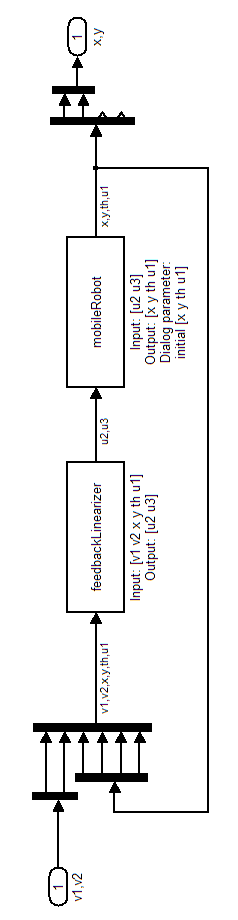
\includegraphics[height=0.75\textheight]{feedbackLinearization.png}
	\caption{State Feedback Input-Output Linearized Mobile Robot.}
\end{figure}

\begin{figure}[htp]
	\centering
	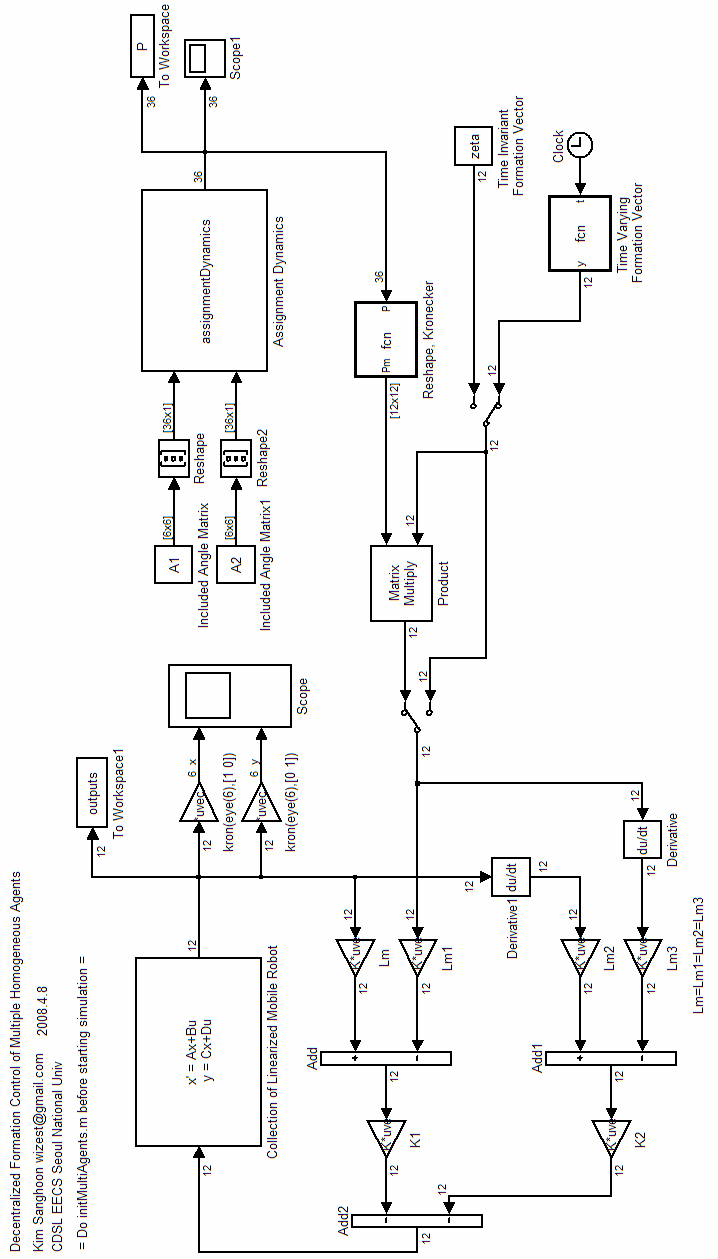
\includegraphics[height=0.95\textheight]{matlabMultiAgents.png}
	\caption{Matlab Implementation of Formation Tracking Control.}
\end{figure}

\subsubsection{makeIncludedAngleMatrix.m}
\begin{footnotesize}
\begin{Verbatim}[fontfamily=cmtt,baselinestretch=0,numbers=left]
function A = makeIncludedAngleMatrix(v)
v = reshape(v,2,length(v)/2);
c = mean(v.').';    % center
l=length(v);
A=zeros(l,l);
s=180/pi;
for i=1:l
    for j=1:l
        psi=v(:,i)-c;   psj=v(:,j)-c;
        if (norm(psi) * norm(psj) == 0)
            A(i,j) = 0;
        else
            val= (psi'*psj) / (norm(psi)*norm(psj));
            A(i,j)=s*real(acos(val));
        end
    end
end
\end{Verbatim}
\end{footnotesize}

\subsubsection{toMatrix.m}
\begin{footnotesize}
\begin{Verbatim}[fontfamily=cmtt,baselinestretch=0,numbers=left]
function X=toMatrix(x)
n=sqrt(length(x));
X=reshape(x,[n n]);
\end{Verbatim}
\end{footnotesize}

\subsubsection{toVector.m}
\begin{footnotesize}
\begin{Verbatim}[fontfamily=cmtt,baselinestretch=0,numbers=left]
function x=toVector(X)
[i j]=size(X);
x=reshape(X,[i*j 1]);
\end{Verbatim}
\end{footnotesize}

\subsubsection{initMultiAgents.m}
\begin{footnotesize}
\begin{Verbatim}[fontfamily=cmtt,baselinestretch=0,numbers=left]
clear all;

zeta=[0 0 -100 -200 100 -200 -200 -400 0 -400 200 -400].';
k11=300;    k12=50;     k21=300;    k22=50;
K1=kron(eye(6),[k11 0;0 k12]);
K2=kron(eye(6),[k21 0;0 k22]);
    
L=[ 0 0 0 0 0 0;    	-.5 1 -.5 0 0 0;   -.5 -.5 1 0 0 0;
    0 -.5 0 1 -.5 0 	0 -.5 -.5 0 1 0    0 0 -.5 0 -.5 1];
Lm=kron(L,eye(2));

Ai=[0 0 1 0; 0 0 0 1; 0 0 0 0; 0 0 0 0];    Bi=[0 0; 0 0; 1 0; 0 1];
Ci=[1 0 0 0; 0 1 0 0];                      Di=[0 0; 0 0];
A=kron(eye(6),Ai);  B=kron(eye(6),Bi);
C=kron(eye(6),Ci);  D=kron(eye(6),Di);

% initial values of mobile robots
z01 =[ 0 0 (150)*cos(90/180*pi) (150)*sin(90/180*pi)]; 
z02 =[ -150 -900 (70)*cos(-70/180*pi) (70)*sin(-70/180*pi)];   
z03 =[ 250 -1600 (100)*cos(-60/180*pi) (100)*sin(-60/180*pi)];   
z04 =[ -300 -1500  (70)*cos(30/180*pi) (70)*sin(30/180*pi)]; 
z05 =[ 150 -800  (20)*cos(90/180*pi) (20)*sin(90/180*pi)];   
z06 =[ -5 -1550  (80)*cos(-120/180*pi) (80)*sin(-120/180*pi)];    
initZ=[z01, z02, z03, z04, z05, z06].';

% assignment dynamics
% A1 from formation vector, A2 from initial outputs
A1=makeIncludedAngleMatrix(zeta);
    tmp=reshape(initZ,4,6);
    tmp=reshape(tmp(1:2,:),12,1);
A2=makeIncludedAngleMatrix(tmp);
\end{Verbatim}
\end{footnotesize}

\subsubsection{assignmentDynamics.m}
\begin{footnotesize}
\begin{Verbatim}[fontfamily=cmtt,baselinestretch=0,numbers=left]
function assignmentDynamics(block)
    setup(block);

function setup(block)
    %% Register number of dialog parameters   
	block.NumDialogPrms = 0;
    %% Register number of input and output ports
    block.NumInputPorts  = 2;
    block.NumOutputPorts = 1;
    %% Setup functional port properties to dynamically
    %% inherited.
    block.SetPreCompInpPortInfoToDynamic;
    block.SetPreCompOutPortInfoToDynamic; 
    block.InputPort(1).Dimensions        = 6^2;
    block.InputPort(1).DirectFeedthrough = false;
    block.InputPort(2).Dimensions        = 6^2;
    block.InputPort(2).DirectFeedthrough = false;
    block.OutputPort(1).Dimensions       = 6^2;  
    %% Set block sample time to continuous
    block.SampleTimes = [0 0];  
    %% Setup Dwork
    block.NumContStates = 6^2;
    %% Register methods
    block.RegBlockMethod('InitializeConditions',    @InitConditions);  
    block.RegBlockMethod('Outputs',                 @Output);  
    block.RegBlockMethod('Derivatives',             @Derivative);  

function InitConditions(block)
    block.ContStates.Data = toVector(eye(6));

function Output(block)
    block.OutputPort(1).Data = block.ContStates.Data;

function Derivative(block)
    A1= toMatrix(block.InputPort(1).Data);
    A2= toMatrix(block.InputPort(2).Data);
    P = toMatrix(block.ContStates.Data);    
    k= 1000;
    dP = P*(P'*A2*P*A1 -A1*P'*A2*P) -k*P*((P.*P)'*P -P'*(P.*P));
    block.Derivatives.Data = toVector(dP);    
\end{Verbatim}
\end{footnotesize}

\subsubsection{Block: Time Varying Formation Vector}
\begin{footnotesize}
\begin{Verbatim}[fontfamily=cmtt,baselinestretch=0,numbers=left]
function y = fcn(t)
zeta=[  0;                  0;
        -100-50*sin(t);    -200-100*sin(t);
        100+50*sin(t);     -200-100*sin(t);
        -200-100*sin(t);    -400-200*sin(t);
        0;                  -400-200*sin(t);
        200+100*sin(t);     -400-200*sin(t)];
y = zeta;
\end{Verbatim}
\end{footnotesize}
	
% 참고문헌
% 참고문헌에 대해 잘 모르는 분들은 주위 사람에게 물어보거나 아래 링크를 참조할 것
% http://faq.ktug.or.kr/faq/참고문헌만들기
\addcontentsline{toc}{chapter}{Bibliography}
\bibliographystyle{amsplain}
\bibliography{document}

% 본문 이후의 쪽들
\backmatter

\newpage\thispagestyle{empty}\mbox{}\newpage

% 국문초록
\begin{KoreanAbstract}
다 개체 동종 시스템의 분산 편대 추종 제어는 최근 몇 년간 많은 연구가 이루어져 왔다. 
이러한 관심은 군사 분야, 모발 센서 네트워크, 지능형 교통 시스템과 같은 
새롭고 흥미로운 응용 사례가 대두됨에 따라 집중되었다. 
분산 편대 제어는 여러가지 이론과 방법으로 연구되어 왔는데 
대부분의 경우 여러 동종 시스템의 상호 연결성을 토대로 라플라스 인접 행렬의 성질로 설명하고 있다.
이러한 접근법은 합의 문제와 동기화 문제와도 관련 깊으며 
이 경우 편대 제어와 유사한 방식으로 안정도를 설명하며 설계 고려 사항을 도출한다. 
본 논문에서, 우리는 분산된 방법으로 여러 대의 동종 비선형 시스템을 다루며 
이 시스템들은 시간에 대해 부드럽게 변하는 상대 기준 위치에 따라 편대를 이룰 수 있고 
또한 전체 그룹은 모든 방향으로 자유롭게 움직이는 것이 가능하다. 
우리의 주요 목표는 위와 같은 편대 추종 제어의 안정도를 해석하고 제어기를 설계하는 것이다. 
그리고 우리는 추가적으로 시스템의 순서 교환을 통해 여러 시스템간 동질성을 이용하는 방법에 대해 논한다. 
	% 다 개체 동종 시스템의 분산 편대 추종 제어는 최근 몇 년간 많은 연구가 이루어져 왔다.
	% 이러한 관심은 군사 분야, 모발 센서 네트워크, 지능형 교통 시스템과 같은
	% 흥미롭고 새로운 응용 사례가 대두됨에 따라 집중되었다. 
	% 분산 편대 제어는 여러 가지 이론과 방법으로 연구되어 왔는데 대부분의 경우 
	% 여러 동종 시스템의 상호 연결성을 토대로 라플라스 인접 행렬의 성질로 설명하고 있다.
	% 이러한 접근법은 합의 문제와 동기화 문제와도 관계가 있는데 이 경우 
	% 편대 제어의 경우와 유사한 방식으로 안정도를 설명하며 설계 고려 사항을 도출한다.
	% 본 논문에서, 우리는 분산된 방법으로 여러 대의 동종 비선형 시스템을 다루며
	% 이 시스템들은 시간에 대해 부드럽게 변하는 상대 기준 위치에 따라 편대를
	% 이룰 수 있고 또한 전체 그룹은 모든 방향으로 자유롭게 움직이는 것이 가능하다.
	% 우리의 주요 목표는 위와 같은 편대 추종 제어의 안정도를 해석하고 제어기를 설계하는 것이다.
	% 그리고 우리는 추가적으로 시스템의 교환을 통하여 여러 시스템의 동질성을 이용하는 것을 논한다.
\end{KoreanAbstract}

\newpage\thispagestyle{empty}\mbox{}\newpage\noindent
% 감사의 글
\begin{KoreanAcknowledgement}
부족한 제자를 관심과 사랑으로 아낌 없이 지도해 주신 
심형보, 서진헌 교수님께 깊은 감사의 말씀을 드립니다. 더불어 학위 논문 심사를
맡아 주신 이범희 교수님께도 심심한 감사의 말씀을 올립니다.
지난 2년간 격려와 애정을 베풀어 주신 제어 및 동역학 연구실의 많은 선후배님께도  
이 기회를 빌어 고마운 마음을 전하고자 합니다.
특히 301동 7층의 연구실을 함께 환희 밝혔던 상보, 홍근, 영준, 태규, Artem에게 
그리고 윗방의 종욱형, 용운형, 재성형, 한성, 현철형에게 
또한 사랑스런 후배 진영, 찬화, 진우, 수범, 성훈에게
덧붙여 졸업한 원민형, 세진, 병인에게 
마지막으로 백주훈, 김정수 박사님께 한 분 한 분 감사의 말씀을 드립니다.

그간 학창 시절을 보람차고 즐겁게 할 수 있었던 커다란 원동력이었고
많은 경험과 기회의 터전이었던 전공학회 핸즈의 선후배님께도 감사의 마음을 표현하고 싶습니다.
마이크로 로봇을 함께 만들며 저의 우상이 되어 주었던 창현형, 즐겁고 재미있는 일이 가득했던 병수형,
항상 밝은 표정으로 묵묵히 따라주었던 환주, 지호 그리고 언제나 친근한 말동무가 되어주었던 승구, 진형에게
특별한 마음을 표현하고 싶습니다. 또한 지금은 각자의 길에서 열심히 노력하고 있는 99학번의 모든 동기와
이름을 모두 열거하기에 자리가 모자랄 정도로 수많은 선후배님께 감사의 마음을 전합니다.

그 외에도 언제나 우울할 틈이 없도록 만들어 주었던 신나는 광하, 
항상 든든한 버팀목이 되어주는 상일 그리고 변치 않는 오랜 나의 친구 재교, 
함께 지내어도 잘 살펴주지 못해 미안한 사촌동생 민우에게도 고마운 마음을 보냅니다.
덧붙여 완전 소중한 나의 누나와 믿음직한 매형, 이쁜이 조카 현서에게 감사의 마음을 전하며
손자의 건승을 기도하시는 할머니께도 고마움을 올립니다.
끝으로 언제나 곁을 함께하며 목표와 의지를 잃지 않게 도와 주었던 사랑하는 소연에게 고마움을 전합니다.

이제 오랜 학업을 뒤로 하고 사회인이 되려 합니다.
많은 분들의 염려와 걱정에 보답하며 자랑스런 상훈이 되도록 항상 처음 그대로의 마음으로 열심히 노력하겠습니다.

마지막 페이지를 덮으며, 
이 모든 저를 있게 하고 그 무엇으로도 대신할 수 없는 더할 수 없이 사랑하는 나의 부모님께 이 논문을 바칩니다.
어머니, 아버지 사랑합니다.
\begin{flushright}
2008년 7월의 어느 깊은 밤에 김상훈 올림
\end{flushright}
\end{KoreanAcknowledgement}



\newpage\thispagestyle{empty} \noindent 
\null \vfill
\begin{center}
\noindent  새로운 삶의 경계를 향해, 나는 걸음을 떼다.\\ 
\end{center}
\vfill



\newpage\thispagestyle{empty}\mbox{}\newpage
\newpage\thispagestyle{empty}\mbox{}\newpage

\end{document}
